% Reproservice prints on G4, which is about 80% of A4.
% With this scale, 12pt font becomes 9.6pt.
% https://student.portal.chalmers.se/doctoralportal/handbook/Doctoral%20Thesis%20Defence/Pages/Layout-of-the-thesis.aspx


% % If we print original on G5 and not rescale it.
% \documentclass[10pt,a4paper,twoside,openright]{book}
% \usepackage[
%    papersize ={169mm, 239mm}
%   ,twoside
%   ,pass
%   ,inner=2cm                % inner margin
%   ,outer=2cm                % outer margin
%   ,bindingoffset=0.8cm       % additional binding offset on the inner side
%   ,bottom=2.4cm
% ]{geometry}                   % Adjust the margins

% If we print original on A4 and rescale it.
\documentclass[12pt,a4paper,twoside,openright]{book}
\usepackage[%                 %
   a4paper
  ,twoside                    %
  ,inner=2.5cm                % inner margin
  ,outer=2.5cm                % outer margin
  ,bindingoffset=1cm       % additional binding offset on the inner side
  ,bottom=3cm
]{geometry}                   % Adjust the margins

\raggedbottom                 % book class spreads floats/paragraphs vertically. That's ugly! Let's disable that.

\synctex=1                    % instead of "pdflatex -synctex=1 main"

\usepackage{lipsum}           % generating fill-in text for this thesis template

\usepackage{ifthen}           % if-then-else (to choose PhD/Lic titles)

\usepackage[utf8]{inputenc}   % unicode letters in the input tex document

\usepackage[T1]{fontenc}      % unicode letters in the output pdf

\usepackage{amssymb, amsmath} % math symbols

% \usepackage{lmodern}          % better font

% \usepackage{microtype}        % micro typesetting (on errors use draft to disable)

\usepackage{booktabs}         % better table formatting

\usepackage[]{graphicx}       % images

\usepackage{tikz}             % simply amazing graphics library for LaTeX
\usetikzlibrary{calc}

\usepackage{fancyhdr}         % fine-tuning of headers
\pagestyle{fancy}

\usepackage{emptypage}        % no page numbers in headers/footers of blank pages between chapters

\usepackage{setspace}         % for \setstretch in captions

\usepackage[%
    margin=0.75cm,            % make captions narrower than the main text
    font={small,stretch=0.80}%%
  ]{caption}                  % captions

\usepackage{subcaption}       % subcaption -- subfigures (replaces subfig)

\usepackage{url}              % handles URLs correctly (e.g. DOI, software links)

\usepackage{wrapfig}          % wrap text around figures

\usepackage[%
  url=true,%                  % print URLs in references, except for the ones removed below
  backend=biber,%             % use biber instead of bibtex
  firstinits=true,
  sorting=none,
  style=numeric-comp,%          % cite as: (Author 2008)
%   maxbibnames=10,%            % max names in bibliography
%   maxcitenames=2,%            % max names in citation
%   mincitenames=1,%            % if there are more than maxcitenames, shrink to this
  backref=true,%              % prints page numbers (wrong with \frontmatter and hypertexnames=false)
%   dashed=false                % do not replace repeated author with a dash in bibliography
]{biblatex}                   % Modern bibtex replacement (bibliography mgmt)

\usepackage[%
%    pdftex%
  ,hidelinks%
  ,linktoc=all%               % part of a ToC entry to be made into a link (section/page/all)
  ,unicode%
  ,bookmarksopen=true%
  ,bookmarksopenlevel=0
  ,bookmarksnumbered=true
  %,hypertexnames=false,%     % Correct ToC hyperlinks even with chapter counter reset, but broken biblatex backref.
                              % Instead of using hypertexnames=false, use \renewcommand on \theHchapter, 
                              % see http://tex.stackexchange.com/a/6099
  %,draft                     % draft can be used to avoid some strange links errors
]{hyperref}                   % links in pdf document

\usepackage{bookmark}         % Create pdf bookmarks in one go

% My packages
\usepackage{todonotes}                              % To do notes and figures
\usepackage{nicefrac}                               % Nice fractions
\usepackage[super]{nth}                             % 1st, 2nd, 3rd, ...
\usepackage{float}                                  % Floats for images
\usepackage{siunitx}                                % SI units
\usepackage{pdfpages}                               % To include pdf's
% \usepackage{fullpage}                               % Use the full page
\usepackage{bm}                                     % Bold matrices
% \usepackage{physics}                                % Extra overrides for physics. Real, imag, vectors, ...

% Commands for matrix and vector quantities.
\newcommand{\matr}[1]{\bm{#1}}     % ISO complying version
\newcommand{\vect}[1]{\mathbf{#1}}

\usepackage{enumerate}                              % enumerate options, roman numbers

\usepackage{csvsimple}                              % Read CSV files for tables

% Nomenclature
% \usepackage{nomencl}
\usepackage{longtable}

\usepackage{dirtytalk}  % Simple quotation
% \usepackage{listings}   % Code highlighting
\usepackage{minted}     % minted is a LaTeX package that provides syntax highlighting using the Pygments library.
\usepackage{afterpage}  % to group floats on same page

\usepackage{mathtools}
\DeclarePairedDelimiter\ceil{\lceil}{\rceil}
\DeclarePairedDelimiter\floor{\lfloor}{\rfloor}
\DeclarePairedDelimiter\abs{\lvert}{\rvert}

\usetikzlibrary{shapes,arrows,positioning,calc}     % For the figures

% % % Biblatex

\addbibresource{library.bib}  % Bibliography file
\renewcommand{\cite}{\parencite}

% % Remove URLs from common (easy-to-find) entries.
% \AtEveryBibitem{%
%   \ifboolexpr%
%     {%
%       test { \ifentrytype{book} }
%       or
%       test { \ifentrytype{inbook} }
%       or
%       test { \ifentrytype{inproceedings} }
%       or
%       test { \ifentrytype{incollection} }
%       or
%       test { \ifentrytype{article} }
%     }
%     {\clearfield{url}}
%     {}%
% }
% % End Biblatex


% % % New environments

% \newenvironment{env-name}[optional-number-of-args]{insert-before}{insert-after}

% \newenvironment{env-name}[optional-number-of-args][default-args]{insert-before}{insert-after}

\newenvironment{abstract}{
  \begin{center}
    {\bfseries Abstract\par}  % \bfseries - some bold font, \par - end of paragraph (as empty line)
  \end{center}
  \quotation                  % extra indent from left and right
  \noindent
}
{\par\endquotation}

\newenvironment{keywords}%
{{\bfseries Keywords:}}%
{\par}%
% % % End new environments


% % Begin page content adjustments for putting more text on pages.
% \renewcommand{\topfraction}{.85}       % max fraction of floats at top
% \renewcommand{\bottomfraction}{.7}     % max fraction of floats at bottom
% \renewcommand{\textfraction}{.15}      % minimal text wrt. figs
% \renewcommand{\floatpagefraction}{.66} % fraction for page of floats. floatpagefraction MUST be less than topfraction
% \renewcommand{\dbltopfraction}{.66}    % fit big float above 2-col. text
% \renewcommand{\dblfloatpagefraction}{.66}
% \setcounter{topnumber}{9}
% \setcounter{bottomnumber}{9}
% \setcounter{totalnumber}{20}
% \setcounter{dbltopnumber}{9}
% \widowpenalty=300                             % widow (at the beginning of page)
% \clubpenalty=300                              % orphans (at the end of page)
% \setlength{\parskip}{0ex plus 0.1ex}  % space between paragraphs
% % End page content adjustments

% % %
% Begin remove page numbers from the "Part I" pages
\fancypagestyle{veryempty}{% no headers, no page numbers
  \fancyhf{} % remove everything
  \fancyfoot{}
  \renewcommand{\headrulewidth}{0pt} % remove lines as well
  \renewcommand{\footrulewidth}{0pt}
}
\makeatletter
\renewcommand\part{%
  \if@openright
    \cleardoublepage
  \else
    \clearpage
  \fi
  \thispagestyle{veryempty}%
  \if@twocolumn
    \onecolumn
    \@tempswatrue
  \else
    \@tempswafalse
  \fi
  \null\vfil
  \secdef\@part\@spart}
\makeatother
% End remove page numbers from the "Part I" pages


% % % % %

% Common things used both in the thesis and in the defence announcement

\newcommand\thesistype{PhD} % PhD or Lic

\newcommand\thesistitle{Auralisation of airplanes considering sound propagation in a turbulent atmosphere}
\newcommand\thesissubtitle{} % if empty leave only {}
\newcommand\thesisauthor{Frederik Rietdijk}

\newcommand{\thesiscoverimage}{../figures/generated/turbulence-parameters/turbulence-1.0-1e-06} % Cover image. Comment away (not leave empty) if not needed
\newcommand{\thesiscoverdescription}{}%Cover: Supervisor for interactive product configuration, see Figure~\ref{fig:kappa-sup} on page~\pageref{fig:kappa-sup}.}  % Leave {} if no description of the cover image needed

\newcommand\thesisdepartment{Architecture and Civil Engineering}
\newcommand\thesiscity{Göteborg}
\newcommand\thesismonth{September} % e.g. January, February...
\newcommand\thesisyear{2017}
\newcommand\thesisisbn{ISBN: 978-91-7597-620-4}
\newcommand{\thesisissn}{%
  \ifthenelse{\equal{\thesistype}{PhD}}%
    {ISSN: 0346-718X}% For PhD it is Chalmers PhD ISSN (call library to double-check)
    {}% For Lic it is Departmental reports ISSN (ask secretary)
}
\newcommand\thesisnumber{4301} % for PhD this is "Ny serie nr" and looks like 3452 (call library to get your number), for Lic it is departmental report number and looks like R001 (ask department secretary)

% Defence information
\newcommand\defenceday{22nd} % e.g. 14th
\newcommand\defencemonth{\thesismonth} % e.g. January, February...
\newcommand\defenceyear{\thesisyear} % e.g. 2009, 2010...
\newcommand\defencetime{10:00} % e.g. 10:00, 13:00...
\newcommand\defenceroom{SB-L516} % e.g. "EA", "HC4"...
\newcommand\defenceaddress{Sven Hultins Gata 6} % from where the \thesislocation can be accessed
\newcommand\defenceopponent{Dr. Stephen Rizzi}
\newcommand\defenceopponentdepartment{Aeroacoustics Branch}
\newcommand\defenceopponentuniversity{NASA Langley Research Center}
     % author, title, etc

\title{\thesistitle}
\author{\thesisauthor}

% \pdfinfo{%
%   /Title (\thesistitle)
%   /Author (\thesisauthor)
% }

% Compression options
% \pdfminorversion=5
% \pdfobjcompresslevel=3  % compression requires \pdfminorversion at least 5
% \pdfcompresslevel=9     % compression requires \pdfminorversion at least 5


\begin{document}

\pagenumbering{alph}

\thispagestyle{empty}

\begin{tikzpicture}[remember picture, overlay]
  \node [anchor=north west, inner sep=0pt]  at (current page.north west)
     {
\includegraphics[width=\paperwidth]{frontmatter/standard-cover-header}};

  % Cover image
  \ifdefined\thesiscoverimage
    \node [inner sep=0pt,anchor=north west]  at
      ($ (current page.north west) + (1.8cm, -7cm) $)
       {\includegraphics[width=11cm]{\thesiscoverimage}};
  \fi

  % Title
  \node [inner sep=0pt,anchor=south west, text width=17cm]  at
    ($ (current page.north west) + (1.8cm, -22.5cm) $)
     {
       \begin{spacing}{2}
         \textnohyphenation{\Huge \bfseries \textls*[40]{\thesistitle}}
        \end{spacing}
     };

  % Name
  \node [inner sep=0pt,anchor=north west, text width=16cm]  at
    ($ (current page.north west) + (1.8cm, -23.5cm) $)
     {\LARGE \textsc{\textls*[80]{\MakeUppercase{\thesisauthor}}}};

  % University
  \node [inner sep=0pt,anchor=north west, text width=16cm]  at
    ($ (current page.north west) + (1.8cm, -25.5cm) $)
     {
     \begin{spacing}{1.05}
     \textit{\large{Department of \thesisdepartment}}
     \par \vspace{0.15cm} \noindent
     \small \textsc{\textls*[80]{CHALMERS UNIVERSITY OF TECHNOLOGY}}
     \par \vspace{0.03cm} \noindent
     \large{Gothenburg, Sweden \thesisyear}
     \end{spacing}
   };

\end{tikzpicture}

\cleardoublepage  % advance two pages

\setcounter{page}{1}  % restart page numbering

\pagenumbering{roman}


\frontmatter                  % roman page numbers

{
\parindent 0 pt
\centering
\thispagestyle{empty}         % no page numbers here

{\small\scshape Thesis for the degree of 
\ifthenelse{\equal{\thesistype}{PhD}}{Doctor of Philosophy}{Licentiate of Engineering}}

\vspace{10 pc}

{\LARGE \thesistitle}
\vskip 1pc

{\large \thesissubtitle}
\vspace{2 pc}

{\large \thesisauthor}

\vfill


\includegraphics[width=30mm,clip]{frontmatter/standard-images/Bildmarke30mm}

\vspace{1cm}

Department of \thesisdepartment

{\scshape CHALMERS UNIVERSITY OF TECHNOLOGY}

Göteborg, Sweden \thesisyear

\clearpage
}


\vspace*{50 pt}
{
  \thispagestyle{empty}         % no page numbers here

  \parindent 0 pt

  \thesistitle

  \thesissubtitle

  \textsc{\thesisauthor}

  \thesisisbn

  \vskip 1pc

  \copyright\enskip \textsc{\thesisauthor, \thesisyear.}

  \vskip 1pc

  \ifthenelse{\equal{\thesistype}{PhD}}{Doktorsavhandlingar}{Licentiatavhandlingar}
   vid Chalmers tekniska högskola

  \ifthenelse{\equal{\thesistype}{PhD}}{%
    Ny serie nr \thesisnumber%
  }{%
    Technical report No. \thesisnumber%
  }

  \thesisissn

  \vskip 1pc

  Department of \thesisdepartment

  Chalmers University of Technology

  SE--412 96 Göteborg, Sweden

  Telephone\enskip+ 46 (0) 31 -- 772 1000

  \vfill

  \thesiscoverdescription

  \vskip 2pc

  Typeset by the author using \LaTeX.

  \vskip 1pc

  Printed by Chalmers Reproservice

  Göteborg, Sweden \thesisyear
}

\clearpage


% \thispagestyle{empty}         % no page numbers here
\vspace*{10 pc}
\hfill{\it to my family}
\vfill
\clearpage


% Add abstract to the ToC
\cleardoublepage              % advance the pages
\phantomsection               % put pdf anchor
\addcontentsline{toc}{chapter}{Abstract}  % add toc line with target at the last anchor
\chapter*{Abstract}
\vspace*{-1cm}                % More space for abstract text
Aircraft noise is a major issue in urban areas and is one of the research topics
within the FP7 SONORUS project. Current methods for determining the impact of
aircraft noise on annoyance and sleep disturbance are based on energetic
quantities disregarding the dynamic character of the sound. To obtain a more
complete representation of annoyance, listening tests with audible aircraft
sound promise to determine the impact of the aircraft sound on people more accurately.

A tool was developed to auralise aircraft noise. The propagation model includes,
aside from the typically considered propagation effects like Doppler shift, a
computationally efficient model to generate sequences of amplitude and phase
fluctuations due to atmospheric turbulence. The method, already used in the
field of wireless communication to predict the performance of wireless
communication links, could be used in the field of acoustics to create more
perceptually valid auralizations. Depending on parameters that are used to
describe the atmospheric turbulence, the amplitude modulations result in clearly
audible modulations and peaks in a spectrogram. Furthermore, the phase
modulations cause additional decorrelation.

An inverse propagation model was developed to compute back from a receiver to
source in time-domain. An automated procedure was developed to extract features
from the resulting signal. These features were then used to directly synthesise
the emission as function of time, and this signal was propagated to the original
receiver resulting in an auralisation that should reproduce the recording
it is based on.

To determine whether the auralisations indeed resembled the recordings, and thus
to validate the auralisation tool, a listening test was conducted. Participants
were asked to rate the similarity of two sounds in a paired comparisons. Two
aircraft types were considered, and the participants were clearly able to
discriminate between them, in case of both the recordings and the auralisations.
However, according to the participants the auralisations did not yet fully match
the recordings.
\todo{rewrite}




% OLD

% An increasing amount of people live in urban environments. The amounts of
% traffic increase as well, a While aircraft have become more quiet over the
% years, there is also more people than ever flying, and thus the amount of people
% exposed to aircraft noise increases.
%
% Noise has a negative impact on humans, it can cause annoyance, distraction,
% sleep disturbance, stress. The impact of sound on humans depends on multiple
% aspects, like the character of the sound as well as expections from those
% exposed to it. Current aircraft noise assessment methods are based on metrics that consider
% only the energy of the sound and not the character. To better predict the impact
% of sound on humans, the audible sound should be considered instead of just a level.
%
% Recordings can be used to investigate the human response to aircraft sound,
% however, with recordings you're limited in the parameters you can very, and thus
% in how you can control a human response experiment. Auralization is a process to
% render a soundfield audible. While originally used to predict the sound inside a
% space, it is now also used to simulate the soundscape of outside spaces.
% Depending on the auralization method one can adjust parameters affecting
% sound generation and propagation. \todo{controlled experiment}
%
% Auralizations have been made of cars, windturbines and aircraft. Typically the
% source synthesis is done using Spectral Synthesis Modelling and the sound
% propagation is based on geometrical acoustics. Spectral Synthesis Modelling
% allows for a detailed sound synthesis, with the limiting factor typically being
% the lack of sufficiently detailed input.
%
% \todo{emission synthesis}
%
% Propagation models typically assume a steady atmosphere as this significantly
% simplifies the modelling as the resulting system is entirely deterministic. In
% practice, atmospheric turbulence, which is of a stochastic nature, affects the
% refractive index of the medium and thus wave propagation.
% % In practice, spatial and temporal fluctuations of windspeed and temperature, that
% % are of a stochastic nature, affect the refractive index of the medium and thus
% % wave propagation. \todo{maybe drop refractive index}
% The effects of atmospheric turbulence on wave propagation are clearly audible.
% It is therefore expected that atmospheric turbulence affects the perceived
% realism of aircraft auralizations and is therefore required to study the impact
% of aircraft sound on humans.
%
% Modelling sound propagation through a turbulent atmosphere is typically
% computationally expensive. Therefore, a simple and fast model was developed
% to account for atmospheric turbulence in auralizations. \todo{something about model}

% \todo{listening tests}
%
% \todo{conclusions}

\vspace{0.1cm}

\textbf{Keywords}: Aircraft noise, Auralization, Outdoor sound propagation, Atmospheric turbulence


\cleardoublepage              % advance the pages
\phantomsection               % put pdf anchor
\addcontentsline{toc}{chapter}{Acknowledgments}  % add toc line with target at the last anchor
\chapter*{Acknowledgments}
The research leading to these results has received funding from
the People Programme (Marie Curie Actions) of the European Union's Seventh
Framework Programme FP7/2007-2013 under REA grant agreement number 290110,
SONORUS "Urban Sound Planner".

Four years ago I began to work on aircraft auralisation at Empa in Switzerland.
Not yet fully grasping the importance of the aircraft noise issue I soon found
out, enjoying aircraft sounds daily, both
at work, and at home! So, thank you to everyone flying in and out of Z\"{u}rich
Airport during that period for the wonderful learning experience!

Thankfully, there was far more than just the annoyance and sleep disturance due to
these aircraft. There were my colleagues at Empa, whom I thank for the
discussions and the introduction to your secret language and its
dialects, some of which were just impossible to understand. You
tried hard and I appreciate the attempts, but I think its safe to say I'll never
speak \say{Switzerdeutsch}. What I will remember is the \say{li} at the end of
words, since it does sound funny :)

Kurt H., I am glad I had you as a supervisor during these years at Empa. I've
learned a lot from you and from our discussions. It was very nice being able to
just walk in, discuss, and write down our ideas. We tried real hard getting to
the bottom of that pile of old seminar abstracts! Reto, thank you also for the
useful discussions, for contributing some decent music to the playlist, and for
ensuring the music was on by the time I got in. Christoph, thank you for helping
with the aircraft and airport \say{things}, and for providing that mountain of
data. It was good to be able to discuss and compare our approaches.

Then, there are my colleagues in the SONORUS project. Four years ago we embarked
on an \say{Urban Sound Planning} journey and faced soundwalks, noise maps,
discussions, presentations, and pubs. And, indeed, our research projects.
Frustrating at times, I am still glad for the experience and our time together.

Time to fly to Sweden: Chalmers. Wolfgang, thank you for the supervision. We did
not meet often, and mails occasionally ended up in a black hole, but the meetings we
had, and the feedback I got, was very useful, thank you! Jens, I recall you said
you \say{had an idea} on auralisation and turbulence. I don't think I could have
imagined at the time what kind of literature would follow. Thank you for that
initial idea, and thank you for the assistence along the way. Finally, I would
like to say thank you to everyone at the division for the talks, discussions,
fikor, puzzle tour(s) and the \say{gezellige} environment!


% % TODO is that also required here?
%
% \vskip 2pc
%
% \noindent \thesisauthor
%
% \noindent \thesiscity, August\  2017  % Since dedication is written a month or more before the actual thesis date, \thesismonth and \thesisyear is not used here.


\cleardoublepage              % advance the pages
\phantomsection               % put pdf anchor
\addcontentsline{toc}{chapter}{List of Publications}  % add toc line with target at the last anchor
\chapter*{List of Publications}
% This page is hand-made. I could not make Biblatex to output the papers the way I wanted.

\begin{refsection}

This thesis is based on the following appended papers:

\begin{description}
% Biblatex \fullcite{Voronov2011} would work, but it uses maxcitenames, not maxbibnames, and there is no obvious way to change maxbibnames locally and change it back afterwards.
\item[Paper~\ref{pap:supervisory}.] Alexey~Voronov, Knut~Åkesson, Anna~Tidstam, Johan~Malmqvist and Martin~Fabian. \emph{Toward better support for authoring and maintaining product configuration constraints.} Submitted (2012).

\item[Paper~\ref{pap:another-one}.] Alexey~Voronov, Knut~Åkesson, Anna~Tidstam and Johan~Malmqvist. \emph{Verification of Item Usage Rules in Product Configuration.} Proceedings of 9th International Conference on Product Lifecycle Management PLM-12, Montreal, Canada, 2012.
\end{description}

\vspace{1cm}

\noindent Other relevant publications co-authored by Alexey Voronov:
\begin{description}
\normalsize
\newcommand{\ME}{{\bfseries Alexey Voronov}}

\item Anna Tidstam, Lars-Ola Bligård, Fredrik Ekstedt, \ME, Knut Åkesson, Johan Malmqvist. \emph{Development of Industrial Visualization Tools for Validation of Vehicle Configuration Rules.} Proceedings of 9th International Symposium on Tools and Methods of Competitive Engineering, pp. 14, 2012.

\item Sajed Miremadi, \ME. \emph{Symbolic Reduction of Guards in Supervisory Control Using Genetic Algorithms.} Technical report. Göteborg: Chalmers University of Technology, 2012.

\item \ME, Knut Åkesson. \emph{Verification of Process Operations Using Model Checking.} Proceedings of IEEE International Conference on Automation Science and Engineering CASE'2009. pp. 415-420, 2009.

\item \ME, Knut Åkesson. \emph{Verification of Supervisory Control Properties of Finite Automata Extended with Variables.} Technical report. Göteborg: Chalmers University of Technology, 2009.

\item \ME, Knut Åkesson. \emph{Supervisory Control using Satisfiability Solvers.} Proceedings of 9th International Workshop on Discrete Event Systems WODES'2008, pp. 81-86, 2008.
\end{description}

\end{refsection}


% \cleardoublepage              % advance the pages
% \phantomsection               % put pdf anchor
% \addcontentsline{toc}{chapter}{List of Acronyms}  % add toc line with target at the last anchor
% \chapter*{List of Acronyms}
% % To find all three-letter acronyms in file kappa/body.tex that are outside of comments: 
% grep -o "[^%]*" kappa/body.tex | grep -o "\b[A-Z][A-Z][A-Z]\b" | sort | uniq

\begin{tabular}{ l c l }

 AI  & -- & Artificial Intelligence\\
 API & -- & Application Programming Interface \\
 BDD & -- & Binary Decision Diagram\\
 BMC & -- & Bounded Model Checking\\
 BOM & -- & Bill of Materials\\
 CNF & -- & Conjunctive Normal Form\\
 CSP & -- & Constraint Satisfaction Problem\\
 CTL & -- & Computation Tree Logic\\
 DNNF & -- & Decomposable Negation Normal Form\\
 sd-DNNF & -- & Smooth Deterministic DNNF\\
 EFA & -- & Extended Finite Automaton\\
 FPT & -- & Fixed Parameter Tractability\\
 FSA & -- & Finite State Automaton\\
 IUR & -- & Item Usage Rule\\
 LTL & -- & Linear Temporal Logic\\
 MDD & -- & Multivalued Decision Diagram\\
 MUS & -- & Minimal Unsatisfiable Subformula\\
 PDM & -- & Product Data Management         \\
 PLM & -- & Product Lifecycle Management   \\
 SAT & -- & Boolean Satisfiability Problem\\
 SCT & -- & Supervisory Control Theory   \\
 SMI & -- & Set of Mutually-Exclusive Required Items\\

\end{tabular}


% % \cleardoublepage              % advance the pages
% % \phantomsection               % put pdf anchor
% % \addcontentsline{toc}{chapter}{Nomenclature}  % add toc line with target at the last anchor
% % \chapter*{Nomenclature}
% % \newpage\chapter*{Nomenclature}

\begin{longtable}[l]{p{50pt} p{300pt} p{50pt}}
% \textbf{Quantity}   & \textbf{Description} & \textbf{Unit} \\
$\alpha$    &   Pure-tone sound attenuation coefficient for atmospheric absorption  &   dB/m \\


\end{longtable}


% add Contents to PDF bookmarks, but do not add it to the 'printed' Contents
\cleardoublepage
\phantomsection
% \pdfbookmark[level]{text-to-display-in-outline}{unique-pdf-anchor-name}, chapter is level 0
\pdfbookmark[0]{Contents}{Contents}

% Table of Contents
\setcounter{tocdepth}{1}\tableofcontents

\mainmatter                   % normal arabic page numbers

% \part{Introductory chapters}

% Headers, footers
\fancyfoot{}                  % clean all
\fancyhead[RE]{\textit{\nouppercase{\rightmark}}}
\fancyhead[RO]{\thepage}
\fancyhead[LE]{\thepage}
\fancyhead[LO]{\textit{\nouppercase{\leftmark}}}

  \begin{refsection}

    \chapter{Introduction}\label{chapter:introduction}


\section{Background}

\subsection{History of aviation}
On December 17th, 1903, the Wright brothers made the first sustained and
controlled flight with a powered, heavier-than-air, aircraft, and in the years
after developed the first practical fixed-wing aircraft, the Flyer III. Their
invention of aircraft controls was a fundamental breakthrough and marked the
beginning of the Pioneer Era of aviation.

The Pioneer Era, lasting until the First World War in August 1914, saw flight
becoming an established technology. Aircraft exhibitions were held,
demonstrations given, and prizes with the intention of encouraging aviation were
offered. Plenty of developments took place in construction, configuration,
controls, propellers and engines. Centres were established for aeronautical
research and flying schools were opened. In 1911 the first aircraft was used for
military purposes by Italy in the Italian-Turkish war and soon after they were
also deployed during the First World War.

In the period between the World Wars airplanes evolved from low-powered biplanes
made from wood and fabric to high-powered monoplanes made of aluminum. Many
aviation firsts occured during this period, like the first transatlantic flight
in 1919, and commercial airlines followed soon on routes like these.

Development and production continued at an ever higher pace during the
the Second World War and saw the development and deployment of jet aircraft
as well as the first turboprop engine that went into mass-production.

After the Second World War commercial aviation grew rapidly, with the first
purpose-built commercial jet airliner scheduled into service in 1952, and the
first sustained and regular service airline operating only 4 years after.
In 1947 a rocket-powered aircraft went through the sound-barrier and
this quickly led to the development of supersonic interceptor aircraft as a
countermeasure against long-range bombers. The development of intercontinental
ballistic missiles and the succesful launch of the Sputnik 1 began the Space
Race increasing again the pace of aeronautical developments.

The year 1969 saw the use of military Vertical/Short Takeoff and Landing
(V/STOL) aircraft, the first humans on the moon, the unveiling of the Boeing
747, and the maiden flight of the Concorde supersonic passenger airliner.
Commercial airliners started using higher bypass-ratios, resulting in better fuel
economy and less noise. \todo{rewrite part}

In the last quarter of the \nth{20} century, the Digital Age, emphasis changed.
Digital computers were used for design and modelling, and digital systems also
started to appear inside the aircraft. Digital fly-by-wire systems improved
manoeuvrability, stability and drag. In-flight management of the flight plan was
being handled by the newly introduced flight management system, reducing the
workload of the crew.

The beginning of the \nth{21} century saw the application of autonomous unmanned
aerial vehicles (UAVs). The first entirely autonomous flight across the Atlantic
became reality and the solar-powered plane Solar Impulse 2 completed a
circumnavigation of the Earth.

\subsection{Urbanisation, transportation and the impact of aviation}
In 2014 54\% of the world population was living in urban areas. % and this proportion is expected to increase to 66\% by 2050 \cite{UnitedNations2014}.
The world population is growing rapidly and it is expected that the given
percentage increases to 66\% by 2050 \cite{UnitedNations2014}, resulting
in higher urban densities.

People not only live closer to eachother than ever before, but also transport
more than before. Transport allows trade and greater spread of people and is
therefore an important aspect for economic growth. People typically commute to
where they work or study, and transport themselves as well for leisure.
Passenger transport is the essence of tourism, and commerce requires the
transport of people to conduct business. Production and consumption of goods and
products can occur at different locations, thus requiring transport.

% https://en.wikipedia.org/wiki/Environmental_impact_of_aviation
While there is a demand for transport, transport also has a negative
impact on our environment.
Aviation contributes to climate change and air and noise pollution, and these
environmental issues have the potential to limit the operation and growth of
airports. Indeed, aircraft noise is already a limiting factor for the capacity of
regional and international airports throughout the world \cite{Zaporozhets2011}.

Being a major user of energy, transport burns most of
the world's petroleum creating air pollution and contributes to global warming and thereby climate change.
Despite more fuel-efficient and less polluting turbofan and turboprop engines,
the rapid growth of air travel in recent years contributes to an increase in
total pollution attributable to aviation. In the European Union, greenhouse gas
emissions from aviation increased by 87\% between 1990 and 2006. By 2020,
aviation emissions are likely to more than double from present levels
\cite{European2006}.
Because of increasing densification the amount of people living nearby airports
increases as well, and these people are affected by air and noise pollution.


% Transportation has negative impacts on the environment.

% At the beginning of the 20th century the first practical aircraft were developed
% and since then developments in aviation went fast.


\subsection{Aircraft noise and human response}
Aircraft noise is noise associated with the operation of airports and in
particular the nature and extent of noise exposure rising from aircraft
operations. It is the single most significant contemporary environmental
constraint for aviation, and is likely to become more severe in the future
\cite{Zaporozhets2011}.

Aircraft noise produced during operations in the vicinity of airports represents
a serious social, ecological, and economic problem. The noise has a negative
impact on people's health, lowers their quality of life, and lessens their
productivity at work \cite{Zaporozhets2011}.



%
%
% Aircraft noise can cause annoyance and sleep disturbance. Currently, annoyance
% and sleep disturbance are predicted using indicators based on time-averaged sound pressure
% levels. To obtain a more complete representation of annoyance one should
% predict the audible aircraft sound and determine the impact of the sound on people.
%
% \subsection{Human response}
%
% Annoyance and sleep disturbance
%
% \subsection{Noise policy}
%
% World Health Organisation
%
%
% Noise control / mitigation
%
% Environmental Noise Policy (END)
%
% Zurich Aircraft Noise Index (ZFI) \cite{Schaffer2012}
%
%
%
% \subsection{Noise prediction}
%
%
%
% \subsubsection{Prediction models}
%
%
% Noise-Power-Distance-tables, or NPD-tables, are the backbone of a wide range of aircraft noise models in use, like the Integrated Noise Model (INM) \cite{Arntzen2011}.
%
% At Empa the noise prediction model FLULA is used, and a new model called sonAIR is in development \cite{sonAIR}.
%
%
%
%
%
% \subsection{The urban environment soundscape}

% \begin{quotation}
% In 450BC Confucius is reputed to have said: "Tell Me and I Will Forget; Show Me and I May Remember; Involve Me and I Will Understand."
% \end{quotation}



% The urban environment contains many different kinds of sounds, coming from sources ranging from cars to cats, ... to the music someone is listening to in his or her living room whilst a window is open.

% Soundscape


\subsection{Auralisation}% of soundscapes}
% \begin{quote}
% Auralisation is the technique of creating audible sound files from numerical data
% \end{quote} \cite{Vorlander2008}.

% TODO: taken from overview paper
% Auralisation is a technique to simulate the audible sound of an object or environment.
Auralisation is a method to render audible virtual sound fields \cite{Kleiner1993}.
The method has been used to simulate the audible sound inside
rooms, but also for the sound of
cars \cite{Forssen2009,Maillard2012,Pieren2015,Hoffmann2016,Hoffmann2016a},
trains \cite{Pieren2016},
windturbines \cite{Pieren2014,Heutschi2014},
fans \cite{Merino2016} and
aircraft \cite{Arntzen2014a, Rizzi2016a, Rizzi2016}. Auralisation of outdoor sources
and environments is a key topic of the VASTCON Technical Working Group \cite{Vastcon}.

% Common reasons for generating auralisations is to determine how new and old spaces sound,

Different auralisation methods exist. Often emission synthesis and sound
propagation are separated. This is not always the case because its not always
possible, like e.g. when using a wave-based method
\cite{Hornikx2016,Georgiou2016,Georgiou2016a}.

Common methods for the emission synthesis are spectral modelling synthesis (SMS)
and granular synthesis. Granular synthesis typically uses grains based on
measurements and is a computationally fast method for synthesis. Spectral
modelling synthesis generates a signal through a superposition of two types of
signal components: tones and noise. Whereas with the granular synthesis method
each grain typically corresponds directly to specific conditions, e.g. the speed
of and distance to the source, with spectral modelling synthesis the synthesis
strategy can be considered separate from the underlying model, and therefore a
emission synthesis model can be established that relates tonal and spectral
components to the operational state of the source.



\subsection{Aircraft noise auralisation}

% TODO: taken from overview paper
Aircraft auralisation has been used to study future aircraft types
\cite{Rizzi2013,Rizzi2016,Rizzi2016a} and flight procedures \cite{Sahai2016} but
also to investigate the perceived unpleasantness of aircraft flyover noise as
function of certain temporal parameters \cite{Pate2017}.

Aspects to consider when simulating the sound of aircraft are the different
noise sources on the aircraft, the state of the aircraft and thereby the state
of these sources, as well as the condition of the environment.
% \subsection{Aircraft emission}
The main noise sources of a turbojet aircraft are jet noise, fan and turbine
noise, combustion noise and airframe noise. In the case of turboprop aircraft
the main source is the propellor\cite{Zaporozhets2011}. Fan or propellor noise
is mostly tonal whereas the other sources are broadband noise.
Which exact sources are most relevant depends on the aircraft type and flight
procedure as well as the position of the source with respect to the receiver due
to directivity of the sources \cite{Bertsch2015}.

The aircraft emission prediction tools found in the ANOPP-Source Functional
Module of ANOPP2 \cite{Lopes2016, Tuttle2017} and INSTANT\cite{Sahai2016b}, which is based
on ANOPP, use established models for the noise prediction of the individual
noise sources. The Heidmann model is for example used for fan noise and the
Stone model for jet noise. The Heidmann model in ANOPP models
five sources explicitly, of which three correspond to emission of tones and two
to emission of broadband noise \cite{Arntzen2014a}. The model outputs for each
of these five sources a spectrum in fractional-octaves.
For broadband synthesis in the NAF\cite{Aumann2015}, power of the tonal
components in each band is divided by the amount of tones in that band.
Nowadays the Heidmann model in ANOPP can output the frequencies and amplitudes
of forward and aft radiated fan tones. Only Buzz-Saw noise is still output in
\nicefrac{1}{3}-octaves.


%
% % TODO: clean up the following
% \todo{cleanup the following}
% To enhance future aircraft operations, the Dutch National Aerospace Laboratory (NLR) wants to have a more comprehensive picture on aircraft noise annoyance.
% A cooperation of the NRL with NASA focuses on expanding the annoyance research capabilities \cite{Arntzen2011}. The NLR and NASA use a common setup, the Virtual Community Noise Simulator (VCNS).
% A helmet with visor is used to present a visual simulation and headphones are used to present binaural flyover noise.
%
% At NASA, Rizzi et al. auralised the flyover noise of a hybrid wing body (HWB) aircraft as well as a reference aircraft, similar to a Boeing 777-200ER.
%
% % To predict an aircraft trajectory the flight mechanics are modelled, instead
%
% At RWTH Aachen University a virtual reality room was developed with... \cite{Schroder2010}
%
%
% Figure \ref{fig:background_aircraft_noise_spectrogram_original} shows a spectrogram of a recorded aircraft passage.
%
% \begin{figure}[H]
%         \centering
%         \includegraphics[width=0.9\textwidth]{../figures/spectrogram_of_measurement}
%         \caption{Spectrogram of a measured aircraft passage. Doppler shifted tones can clearly be seen.}
%         \label{fig:background_aircraft_noise_spectrogram_original}
% \end{figure}
%


\newpage
\section{Aim}

% \subsection{Aim}

The aim of the thesis is to develop a tool to simulate the audible sound of
aircraft in an urban environment, so that new methodologies can be developed to
assess annoyance and sleep disturbance due to aircraft noise.

There's a large variation of different aircraft in use nowadays, that could each
be perceived differently. An additional constraint is therefore that the tool
should be able to simulate the audible sound of the current fleet of aircraft.


\todo{Check!}

The aim of my research is to develop a tool for the auralisation of aircraft noise in 
an urban environment. This tool can then be used to determine better annoyance 
and sleep disturbance indicators and can then be used in conjunction with a noise prediction 
model like sonAIR to give better a better estimate on how many people are affected by aircraft noise and how severe.

The auralisation tool has to support a typical urban situation where shielding 
and reflections may play an important role and should include correct over-head 
directional information. The work is therefore divided in three parts:

\begin{itemize}
 \item Development of an aircraft source synthesiser
 \item Development of propagation model
 \item Installation of reproduction system for auralisation.
 \end{itemize}

% \section{Thesis structure}
\section{Outline}
The thesis is structured as follows.
\newline
\newline
Chapter \ref{chapter:theory} provides an overview of theory required to understand the concepts that are used throughout the thesis.
Discussed the basics of sound, signal processing, auralisation, previous work on aircraft auralisation and emission synthesis, and finally atmospheric turbulence.
\newline
\newline
Chapter \ref{chapter:tool} describes the auralisation tool that was developed. The propagation model is explained as well as the algorithm that is used to extract features from recordings and synthesise aircraft sounds based on that.
\newline
\newline
Chapter \ref{chapter:turbulence} gives an extensive overview on a novel algorithm for simulating fluctuations due to atmospheric turbulence and how to apply this algorithm in auralisations.
\newline
\newline
Chapter \ref{chapter:test} aims to answer the question whether the auralisation tool provides sufficiently plausible auralisations
\newline
\newline
Finally, the work is summarised in Chapter \ref{chapter:conclusions} and future work is suggested.


\section{Limitations}





% Theory
\chapter{Theory}\label{chapter:theory}
\section{Sound}

A repetitive variation about a central value of some quantity is called an
oscillation. Oscillations of mechanical nature are vibrations. An
oscillation travelling through a medium and transferring energy is a wave. Sound
is then a mechanical wave travelling through a fluid medium. Furthermore, only
those oscillations that can be perceived by the human brain are typically
considered sound.
Being a small repetitive perturbation about the barometric
mean pressure of the medium, the fluctuating or dynamic part of the pressure,
denoted sound pressure, is typically many orders smaller than the mean
pressure.

In the \nth{17} century Newton proposed a model for sound waves in elastic media
in his Principia. Already aware that the humidity of the air influences the
speed of sound, Newton assumed an isothermal process for the wave motion and
thereby computed incorrect values for the speed of sound. Laplace gave the
correct derivation of the classical wave equation, describing the wave motion as
a adiabatic process. In the \nth{19} century Kirchoff described the motion of a
rigid body in an ideal fluid and Helmholtz gave a time-independent form of the
wave equation. These were some of the important foundations for the classical
theory of sound.
% A limitation of the developed theory was the lack of sound generation models. In
% the classical theory sound was only generated through a vibrating solid
% boundary. In the 1950s
In this section a brief overview is given of sound. Discussed are sound
generation, propagation, and the effect of flow.

\subsection{Wave equation}\label{sec:theory:sound:wave}
% In his Principia, Newton gave an description of sound and a value of the speed of sound.
The wave equation is a differential equation for describing waves and is used
throughout physics. In the \nth{18} century d'Alembert discovered the
one-dimensional wave equation, and a couple of years later Euler presented the
three-dimensional wave equation. The acoustic wave equation describes the motion
of sound waves and can be derived from the fundamental laws of fluid dynamics \cite{Arntzen2014a, Rienstra2017}.

\subsubsection*{Mass and momentum conservation}
The mass conservation or continuity equation is given by
% Mass conservation equation
\begin{equation}\label{eq:theory:sound:wave:mass}
 \frac{\partial \rho}{\partial t} + \nabla \cdot \rho \vect{u} = m
\end{equation}
with $\rho$ the density of the medium, $t$ the time, $\vect{u}$ the flow velocity
vector, $m$ the mass and $\nabla = \left( \frac{\partial}{\partial
x_1},\frac{\partial}{\partial x_2},\frac{\partial}{\partial x_3} \right)$.
The momentum conservation equation is
% Momentum conservation equation
\begin{equation}\label{eq:theory:sound:wave:momentum}
 \frac{\partial}{\partial t} \rho \vect{u} + \nabla \cdot \left(\matr{P} + \rho \vect{u} \vect{u}  \right) = \vect{f} + m \vect{u}
\end{equation}
where $\vect{u} \vect{u}$ is a dyadic product\footnote{The dyadic product of the vectors $\vect{a}$ and $\vect{b}$ is the tensor $\vect{a}\vect{b}=a_i b_j$}, $\vect{f}$ the external force
density and $\matr{P}$ the fluid stress tensor. The fluid stress tensor relates the pressure $p$ and the viscous stress tensor $\matr{\tau}$ by
% Viscous stress tensor
\begin{equation}
  \matr{P} = p \matr{I} - \matr{\tau}
\end{equation}
where $\matr{I}$ is a unit tensor. Viscous stresses are small compared to inertial
forces. Ignoring them, and rewriting equation
\ref{eq:theory:sound:wave:momentum} using equation
\ref{eq:theory:sound:wave:mass}, we obtain the following form for the momentum conservation equation
\begin{equation}
 \rho \left( \frac{\partial \vect{u}}{\partial t} + \left( \vect{u} \cdot \nabla \right) \vect{u} \right) + \nabla p = \vect{f}
\end{equation}

\subsubsection*{Linearisation}
Sound is a small perturbation of a steady state, and so we can apply linearisation to obtain a wave equation.
Ignoring the source term at the right-hand side (thus considering the homogeneous solution), the linearised versions of the mass and momentum equations are given by
% Linearised versions of the homogeneous (= without source terms) mass and momentum equations
\begin{align}
 \frac{\partial \rho'}{\partial t} + \vect{u_0} \cdot \nabla \rho' + \rho_0 \nabla \cdot \vect{u'} = 0  \label{eq:theory:sound:linearisation:mass} \\
% \end{equation}
% \begin{equation}
 \rho_0 \left( \frac{\partial \vect{u'}}{\partial t} + \left(\vect{u_0} \cdot \nabla \right) \vect{u'}\right) + \nabla p' = 0 \label{eq:theory:sound:linearisation:momentum}
\end{align}
with the fluctuating components of the variables denoted with a prime and the steady components subscripted with a zero.

\subsubsection*{Speed of sound}
Viscosity is neglected and thereby also heat transfer. The fluid is considered to behave
adiabatic and thus the following relation between pressure and density
fluctuations can be used
% Adiabatic relation between pressure and density fluctuations
\begin{equation}
  p' = c^2 \rho'
\end{equation}
where $c$ is the speed of sound
% Speed of sound for adiabatic process
\begin{equation}
  c = \sqrt{ \left( \frac{\partial p}{\partial \rho} \right)_{s} }
\end{equation}
The subscript $s$ indicates an isentropic (constant entropy $s$) or adiabatic process.
In general, the speed of sound is given by $c = \sqrt{\frac{K}{\rho}}$ where $K$
is the bulk modulus of the medium. For ideal gases the bulk modulus is $K=\gamma
p$ where $\gamma=C_p/C_v$ is the ratio of specific heat capacities at constant
pressure $C_p$ and constant volume $C_V$.

\subsubsection*{Convective wave equation}
A mean flow has an effect on sound generation and propagation.
The material derivative $D/Dt$ is defined as
\begin{equation}
  \frac{D}{Dt} = \frac{\partial}{\partial t} + \vect{u} \nabla
\end{equation}
and is a time derivative of some physical quantity for a portion of a material moving with a velocity $\vect{u}$.

Taking the material derivative of the linearised mass conservation equation and subtracting the divergence of the
linearised momentum conservation equation results in the convective wave equation.
% \begin{equation}
%   \frac{\partial^2 \rho'}{\partial t^2} + \frac{\partial}{\partial t} \left( 2 \left( \vect{u}_0 \cdot \nabla \right) \rho' \right) + \left( \vect{u}_0 \cdot \nabla \right) \left( \vect{u}_0 \nabla \rho' \right) - \nabla^2 p' = 0
% \end{equation}
Assuming an adiabatic process, the convective wave equation then becomes
\begin{equation}
  \frac{\partial^2 \rho'}{\partial t^2} + \frac{\partial}{\partial t} \left( 2 \left( \vect{u}_0 \cdot \nabla \right) p' \right) + \left( \vect{u}_0 \cdot \nabla \right)^2 p' - c^2 \nabla^2 p' = 0
\end{equation}

\subsubsection*{Classical wave equation}
The convective wave equation considers a flow with a velocity $\vect{u}$. If the velocity is zero, the equation reduces to the classical wave equation
\begin{equation}\label{eq:theory:sound:wave:classic}
 \frac{1}{c^2} \frac{\partial^2 p'}{\partial t^2} - \nabla^2 p' = 0
\end{equation}

\subsubsection*{Harmonic wave}
In acoustics harmonic waves in the following complex form are typically considered
\begin{equation}
  p' (\vect{x}, t) = \hat{p} \left(\vect{x}\right) \exp{\left(j \omega t \right)}
\end{equation}
where $\hat{p} \left(\vect{x}\right)$ is the amplitude of the wave and $\omega=2 \pi f$ the angular frequency.

\subsubsection*{Helmholtz equation}
Inserting the (derivatives of) a harmonic wave in the wave equation results in
the Helmholt equation
\begin{equation}\label{eq:theory:sound:wave:helmholtz}
 \left( \nabla^2 + k^2 \right) \hat{p} = 0
\end{equation}
where $k=w/c$ is the wavenumber.

\subsubsection*{Plane wave solution}
The solution to the wave equation in one dimension is
\begin{equation}
  p'(x,t) = p'_{+} (t-x/c) + p'_{-} (t+x/c)
\end{equation}
where $p'_{+}$ and $p'_{-}$ are respectively a right and left travelling function.

\subsubsection*{Spherical wave solution}
A solution in three dimensions assuming spherical symmetry is the spherical wave solution
\begin{equation}
  p'(r,t) = \frac{1}{r} p'_{+} (t-r/c) + \frac{1}{r} p'_{-} (t+r/c)
\end{equation}
and looks similar to the plane wave solution. In this expression $r$ is the
distance travelled by the wave. The spherical wave solution represents the sum
of a wave propagating out from the origin and that of a wave propagating towards
the origin. In acoustics only the outgoing wave is typically kept. Contrary to
a plane wave the pressure of a spherical wave decreases with $1/r$.

\subsubsection*{Wave equation with source terms}
The above solutions considered a homogeneous wave equation and therefore do not
take into account any source terms. Linearisation of the mass and momentum equations
would have resulted in a unsteady mass injection $m'$ and unsteady external
force $\vect{f'}$. The wave equation with these terms is
\begin{equation}
   \frac{1}{c^2} \frac{\partial^2 p'}{\partial t^2} - \nabla^2 p' = \frac{\partial m'}{\partial t} - \nabla \cdot \vect{f}'
\end{equation}
In general a source term can be written as a source $s(\vect{x}, t)$.

\subsubsection*{Green's function}\label{sec:theory:sound:green}
The simplest possible source is a point source that is represented by a Dirac
delta function $\delta(\vect{x}-\vect{x}_0)$ where $\vect{x}_0$ is the position
of the point source. A Green's function is a solution or impulse response of an
inhomogeneous linear differential equation.
Therefore, the solution of the wave equation with such a point source excitation is a Green's function.
For a harmonic point source the Green's function $\hat{G}$ should satisfy
\begin{equation}
  \left( \nabla^2 + k^2 \right) \hat{G} = - \delta \left( \vect{x} - \vect{x}_0 \right)
\end{equation}
Note that because a harmonic point source is considered the Helmholtz equation
is used. The solution of this inhomogeneous Helmholtz equation is again an
ingoing and outgoing spherical wave. Because of causality we consider only the
outgoing wave. In free field the Green's function of this outgoing wave is
\begin{equation}
  \hat{G} = \frac{\exp{\left(jkr\right)}}{4 \pi r}
\end{equation}
with $r = \left| \vect{x} - \vect{x}_0 \right|$ the distance from point source to receiver.
% The point source represented by a Dirac delta pulse is a monopole point source of unit amplitude
% and the resulting field is a monopole field.

% Free-field solution
% \begin{equation}
%  G = \frac{1}{4 \pi r} \delta \left( t - \tau - \frac{r}{c} \right)
% \end{equation}

\subsection{Aerodynamic sound sources}\label{sec:theory:sound:aerodynamic}
The classic wave equation cannot describe aerodynamic sources. Lighthill
provided the theory to take into account aerodynamic sources. The aero-acoustic
analogy of Lighthill is the idea of representing a fluid mechanical process that
acts as an acoustic source by an acoustically equivalent source term.

% He drew an analogy between the non-homogeneous versions of the fluid equations and the classical
% wave equation including the single acoustic source term.

Taking the time derivative of the homogeneous version of the mass conservation
equation (eq. \ref{eq:theory:sound:wave:mass}) and the divergence of the
homogeneous version of the momentum conservation equation (eq.
\ref{eq:theory:sound:wave:momentum}), then subtracting one from another, and
finally subtracting from both sides of the equation $c^2 \nabla^2 \rho$, results in the Lighthill
equation
\begin{equation}
  \frac{\partial^2 \rho}{\partial t^2} - c^2 \nabla^2 \rho = \nabla^2 \matr{T}
\end{equation}
where $\matr{T}$ is the Lighthill stress tensor
\begin{equation}
  \matr{T} = \rho \vect{u}\vect{u} + \left( \left( p - c^2 \rho \right) \matr{I} - \matr{\tau}  \right)
\end{equation}

Lighthill's acoustic analogy has the limitation that the source field is not
coupled to the acoustic field. That means situations where feedback occurs,
i.e., the acoustic field modifies the flow field and vice versa, cannot be
treated.


The Mach number $M = v / c$ represents the ratio of the flow velocity to the
local speed of sound.



\subsection{Elementary sources}

The elementary sources 

\missingfigure{Figure of monopole, dipole and quadrupole}

\subsubsection*{Monopole}

Volume source
%
% \begin{equation}
%  \frac{d^2 \rho'}{dt^2}
% \end{equation}

\begin{equation}
 p' \left(\vect{x},t\right) = \frac{\dot{m} \left(\vect{y}, t-r/c\right)}{ 4 \pi r}
\end{equation}
where $\dot{m} = \partial m / \partial t$ is the time derivative of the unsteady mass flow $\dot{m}$.

\subsubsection*{Dipole}

\begin{equation}
 p' \left(\vect{x}, t\right) =
\end{equation}


\subsubsection*{Quadrupole}

Moment

\subsubsection*{Multipoles and spherical harmonics} % TODO Unless I would write a piece about Ambisonics I have no need for this so could skip it


\missingfigure{Multipoles and spherical harmonics}

Ambisonics


\subsection{Moving source}
The sound field produced by a moving source is different from that of a fixed source.

\subsubsection{Doppler shift}
A commonly known effect related to movement is the Doppler shift.
Movements of source, receiver and medium can cause
Doppler shifts. If we consider a moving harmonic point source, $S(t) = \hat{S}_0
\exp{\left(j\omega_0 t\right)} $, in a homogeneous fluid at rest, then the sound
field is given by
\begin{equation}
  p'(\vect{x},t) = \sum_{t_e} \frac{\hat{S}_0 \exp{\left(j \omega_0 t_e\right)}}{4\pi r \left(t_e\right) \abs{1-M_r (t_e)}}
\end{equation}
and represents a summation of the sound pressure contributions at all emision
times $t_e$. The Mach number $M_r = \vect{M} \cdot \vect{e}_r = M \cos{\theta}$ is
the projection of the Mach number of the source in the direction towards the
receiver. The Mach number of the source is $\vect{M}=\vect{v}/c$ and
$\vect{e}_r=\vect{r}/r$ is the unit vector pointing towards the receiver.
If we consider a moving source and fixed receiver, then the instantaneous
frequency is given by
\begin{equation}
  \omega = \frac{\omega_0}{1 - M_r(t_e)}
\end{equation}
% with $M_r(t_e) = M(t_e) \cos{\theta(t_e)}$.

\subsubsection{Convective amplification}
Another effect that occurs and is especially relevant for fast-moving sources is
convective amplification.

\cite{Dowling1976}

\missingfigure{Convective amplification illustration}





% \chapter{Sound propagation}


\subsection{Atmospheric attenuation}\label{sec:theory_sound_atmospheric_attenuation}
Soundwaves are attenuated due to relaxation processes in the medium.
A model for atmospheric attenuation is given in Part 1 of ISO 9613-1:1993\cite{ISO9613-1}.
The attenuation coefficient $\alpha$, in dB/m, is given by
\begin{align}\label{eq:theory:sound:atmospheric-attenuation}
 \alpha &= 8.686 f^2 \Biggl( \left[ 1.84 \times 10^{-11} \left(\frac{p_r}{p_a}\right)^{-1} \left(\frac{T}{T_0}\right)^{1/2} \right] + \left(\frac{T}{T_0}\right)^{-5/2} \nonumber \\ 
 &\times \Biggl\{ 0.01275 \left[ \exp{\frac{-2239.1}{T}} \right]  \left[f_{r,O} + \frac{f^2}{f_{r,O}} \right]^{-1} \nonumber \\
 &+ 0.1068 \left[ \exp{\frac{-3352.0}{T}} \right] \left[ f_{r,N} + \frac{f^2}{f_{r,N}} \right]^{-1} \Biggr\} \Biggr) 
\end{align}
and is a function of the ambient temperature in kelvin $T$, the reference
temperature $T_0=293.15$ K, the ambient pressure $p_a$ in kilopascal, the
reference pressure $p_r=101.325$ kPa and the relaxation frequencies for oxygen 
$f_{r,O}$ and nitrogen $f_{r,N}$.
The relaxation frequency of oxygen is given by
\begin{equation}
 f_{r,O} = \frac{p_a}{p_r} \left( 24 + 4.04 \cdot 10^4 h \frac{0.02 + h}{0.391 + h}  \right)
\end{equation}
and the relaxation frequency of nitrogen by
\begin{equation}
 f_{r,N} = \frac{p_a}{p_r} \left( \frac{T}{T_0} \right)^{-1/2} \cdot \left( 9 + 280 h \exp{\left\{ -4.170 \left[ \left(\frac{T}{T_0} \right)^{-1/3} -1 \right] \right\} } \right)
\end{equation}
Both depend on the molar concentration of water vapour $h$, given by
\begin{equation}
 h = h_r  \frac{p_{sat}}{p_a}
\end{equation}
The molar concentration of water vapour is a function of the saturation pressure
\begin{equation}
 p_{sat} = 10^C \cdot p_r
\end{equation}
where 
\begin{equation}
 C = -6.8346 \cdot \left( \frac{T_{01}}{T} \right)^{1.261}  + 4.6151
\end{equation}
In this equation $T_{01}$ is the triple-point isotherm temperature of 273.16 K.

The standard furthermore mentions the following expression for the speed of sound
\begin{equation}
c = 343.2 \left( \frac{T}{T_0} \right)
\end{equation}

\begin{figure}[H]
        \centering
        \includegraphics[]{../figures/generated/sound/attenuation}
        \caption{Atmospheric attenuation as function of frequency for a standard atmosphere.}
        \label{fig:theory:sound:attenuation}
\end{figure}

\newpage
\subsection{Reflections}
Sound hitting a boundary between materials of different impedance may be
transmitted, reflected or absorbed. When sound is transmitted the incident wave
is partially refracted. Sound reflected by a smooth surface results in a
specular reflection, and sound reflected on a rough surface results in a diffuse
reflection. In outdoor situations sound is typically reflected by the ground
surface and other obstacles like buildings. The sound pressure at a receiver is
then the sum of the direct contribution as well as indirect contributions from
reflections. Due to this superposition strong interference effects may occur.

\subsubsection*{Impedance}
An impedance is a complex ratio between two interdependent dynamic quantities
and describes the resistance to a direct flow (resistance) and alternating flow
(reactance). The specific acoustical impedance of a material is the ratio of the
sound pressure to the particle velocity normal to the surface $Z_{s} =
p/\vect{u}$. The specific acoustical impedance of a material or surface
normalised by the impedance of air $Z_{s, air} = \rho c$ is called the
normalised specific acoustic impedance. This impedance is typically used to
characterise surfaces, and is what impedance in the following text refers to.

Multiple models are available for the prediction of the impedance of a surface.
Attenborough et. al. made a comparison of impedance models and recommends the
Delany and Bazley one-parameter model for predicting outdoor ground impedance
\cite{Attenborough2011a}. The empirical one-parameter model by Delaney and
Bazley is widely used and depends on the flow resistivity of the material
$\sigma$ and the frequency $f$
\begin{equation}\label{eq:theory:sound:impedance:db}
 Z = 1 + 9.08 \left( \frac{1000f}{\sigma}\right)^{-0.75} - 11.9 j \left( \frac{1000f}{\sigma}\right)^{-0.73}
\end{equation}
Flow resistivity describes how difficult it is for air to flow through a
surface. Values for surfaces can vary significantly, with average values ranging
from \SI{29}{\kilo\pascal\second\per\square\meter} for snow to
\SI{200000}{\kilo\pascal\second\per\square\meter} for painted concrete. Grass
has an average flow resistivity of
\SI{200}{\kilo\pascal\second\per\square\meter} \cite{Crocker1997}.
Furthermore, a surface is called locally reacting if at a certain point the
particle velocity $\vect{u}$ depends only on the sound pressure $p$ at that
point. In case it doesn't the surface has an extended reaction.
Figure \ref{fig:theory:sound:impedance} shows the impedance of grass according to the Delaney and Bazley model.
% TODO drop or expand?

\begin{figure}
        \centering
        \includegraphics[]{../figures/generated/sound/impedance}
        \caption{Impedance for grass with a flow resistivity of \SI{200}{\kilo\pascal\second\per\square\meter} according to Delany and Bazley one-parameter model.}
        \label{fig:theory:sound:impedance}
\end{figure}


%
% Another example of a model is the 2-parameter model by Attenborough. In this model, the impedance is given by
% \begin{equation}\label{eq:theory:sound:impedance:att}
%  Z = \frac{\left( 1-j\right) \sqrt{\sigma/f}}{\sqrt{\pi \gamma_0 \rho_0}} - \frac{jc\alpha}{8 \pi \gamma_0 f}
% \end{equation}
% and depends on the speed of sound in air $c_0$, the density of air $\rho_0$, $\alpha$, $\gamma_0$ and again the flow resistivity $\sigma$ and frequency $f$.

%
% Table \ref{tab:theory:sound:impedance:flow-resistivity} lists co
%
%
% \begin{tabular}{l c}
% Team              & P & W & D & L & F  & A & Pts \\
% \hline
% Manchester United & 6 & 4 & 0 & 2 & 10 & 5 & 12  \\
% Celtic            & 6 & 3 & 0 & 3 &  8 & 9 &  9  \\
% Benfica           & 6 & 2 & 1 & 3 &  7 & 8 &  7  \\
% FC Copenhagen     & 6 & 2 & 1 & 3 &  5 & 8 &  7  \\
% \end{tabular}


% \newpage
\subsubsection{Reflection coefficient}
The pressure reflection coefficient describes the ratio between the sound
pressure of an incident wave $p_i$ and the pressure of the reflected wave $p_r$
and considers a wave incident on an infinite plane that is locally
reacting and has impedance $Z$
\begin{equation}
  R = \frac{p_r}{p_i}
\end{equation}
The plane wave reflection coefficient gives the ratio of incident and reflected pressure assuming the incident wave is plane
\begin{equation}\label{eq:theory:sound:reflection:plane}
  R = \frac{Z\cos{\theta}-1}{Z\cos{\theta}+1}
\end{equation}
and is a function of the angle of incidence $\theta$ of the incident wave.
If the source is relatively close to the reflecting surface,
then typically the wave front is not plane. In such case a spherical wave
reflection factor is used that considers an incident spherical wave.

The impedance and reflection coefficient models together with their parameters
determine in computations how much sound is reflected and how much is
transmitted or absorbed. Because the reflection coefficient is complex-valued
the reflected contribution may have not only a different magnitude than the
direct contribution, but also an additional frequency-dependent phase shift or
propagation delay. Surfaces that attenuate and phase shift the reflected wave
are called acoustically soft surfaces. In case the normalised impedance
approaches infinity, neither attenuation nor phase shift occur, and the surface
is considered acoustically hard. Figure \ref{fig:theory:sound:reflection} shows
both the absolute value and the phase angle of the plane wave reflection angle
as function of frequency and angle of incidence.

% Another commonly used reflection coefficient is the spherical wave reflection coefficient.

% The spherical reflection coefficient is given by
% \begin{equation}\label{eq:theory:sound:reflection:spherical}
%  Q = R \left(1 - R \right) F
% \end{equation}
% with
% \begin{equation}
%  F = 1 - j \sqrt{ \pi} w e^{-w^2} \mathrm{erfc} \left( j w \right)
% \end{equation}
% and
% \begin{equation}
%  w = \sqrt{-j k r  \left( 1 + \frac{1}{Z} \cos{\theta} - \sqrt{1 - \left( \frac{1}{Z} \right)^2} \sin{\theta} \right) }
% \end{equation}

\begin{figure}
%     \centering
    \begin{subfigure}{\textwidth}
        \includegraphics{../figures/generated/sound/reflection-abs}
        \caption{Absolute value of the reflection coefficient.}
    \end{subfigure}
    ~
    \begin{subfigure}{\textwidth}
        \includegraphics{../figures/generated/sound/reflection-angle}
        \caption{Phase angle of the reflection coefficient.}
    \end{subfigure}
    \caption{Absolute value and phase angle of the plane wave reflection angle as function of both frequency and angle of incidence. The impedance was calculated using equation \ref{eq:theory:sound:impedance:db} and for the flow resistivity the average value for grass was chosen.}
    \label{fig:theory:sound:reflection}
\end{figure}

\subsubsection{Ground effect}
In outdoor situations the ground is typically providing the second-largest
contribution and is important when considering an elevated source. As mentioned
before, impedances of surfaces can vary significantly, and this is especially
the case for the ground surface. Spectrograms of recordings of aircraft often
show a distinct interference pattern called the Lloyd's mirror effect. Figure
\ref{fig:theory:sound:reflection:ground} shows a (synthesised) example of the
Lloyd's mirror effect as caused by an elevated moving source.

\begin{figure}
%     \centering
    \begin{subfigure}{\textwidth}
        \includegraphics{../figures/generated/sound-mirror-effect/hard}
        \caption{Hard surface.}
    \end{subfigure}
    ~
    \begin{subfigure}{\textwidth}
        \includegraphics{../figures/generated/sound-mirror-effect/soft}
        \caption{Soft surface.}
    \end{subfigure}
    \caption{Superposition of the direct contribution and ground-reflected contribution results in an interference pattern known as the Lloyd's mirror effect.}
    \label{fig:theory:sound:reflection:ground}
\end{figure}
% TODO interference pattern is shifted}

% A prominent reflection is the reflection with the ground. When the
% reflecting surface is sufficiently hard the Lloyd's
% mirror effect can be heard.


% \begin{figure}[H]
%         \centering
%         \includegraphics[width=0.9\textwidth]{../figures/ipynb/theory_reflections_mirror_effect/figure1}
%         \caption{Spectrogram of a white noise source flying at a height of 100 meters over an acoustically hard surface. The spectrogram clearly shows the Lloyd's mirorr effect.}
%         \label{fig:theory_reflections_mirror_effect}
% \end{figure}

% \missingfigure{SPL relative to free field comparison}


\subsubsection{Multiple reflections and shielding} % TODO don't talk about shielding?
In urban environments there are more reflecting surfaces besides the ground.
Buildings can reflect sound and shield as well. In courtyards or street canyons
multiple reflections and strong rerverberance may occur.

Sound can be considered as a ray if the wavelength of the sound is much smaller
than the characteristic lengths of the objects or geometries. % TODO: move sentence

Assuming sound can be described as a ray, a raytracer could be used to determine
the immission at a receiver position, taking into account refractions and
reflections. Raytracers are commonly used in room acoustics but also in
environmental acoustics for noise prediction.

The image source method is a computationally fast algorithm for taking into
account reflections and uses the concept of mirror sources
\cite{Allen1979,Mechel2013}. Mirror sources are found by mirroring the original
source with respect to the reflective surface that is considered. Higher-order
mirror sources can be found by repeating the process, mirroring the previous
order mirror source with respect to another surface. Care should be taken to
determine whether there is in fact line-of-sight between a mirror-source and the
receiver.

When neither source nor receiver move, the image sources have to be determined
only once, and their validity, that is, line-of-sight between image source and
receiver, needs to be checked only once as well. If instead the receiver moves,
line-of-sight will have to be checked as function of time. When both move, both
the mirror source search as well as the line-of-sight validation has to be
performed as function of time. An interesting question is how to connect image
sources at one instance in time to the image sources the next instance,
considering sources can appear and disappear over time. If only the source
moves, it may be more interesting to consider mirror receivers instead of miror
sources.

% In urban environments multiple reflections generally occur.


% \subsection{Descriptors}







\newpage\section{Signal processing}
In the previous chapters we looked at how sound is generated and propagated, and
we discussed also several aircraft emission models.
We now would like to synthesise the sound of aircraft. This requires generating
signals and modifying them. Therefore, we will first discuss certain signal
processing techniques that are useful or required to develop auralisations.


In this chapter we consider all operations to be in time and/or frequency
domain. Generally, these operations also apply on other domain pairs, like for
example space and/or wavenumber domain.


\newpage
\subsection{Fourier transform}
The Fourier transform decomposes a signal into complex exponentials with different frequencies that the signal is made up of.

The (forward) Fourier transform can be defined as
\begin{equation}
 X(f) = \int_{-\infty}^{\infty} x(t) e^{-j 2 \pi f t} \mathrm{d} t
\end{equation}
where $x(t)$ is a signal in the time-domain, $f$ the frequency of the complex exponential and $j^2=-1$.
Often the complex exponent $e^{-j 2 \pi f t}$ is written as $e^{-j \omega t}$ where $\omega$ is the angular frequency.
Typically, $\mathcal{F} \left\{ x(t) \right\}$ is used to denote the Fourier transform of the function $x(t)$.

To go from frequency to time-domain we can use the inverse Fourier transform which is defined as
\begin{equation}
 x(t) = \int_{-\infty}^{\infty} X(f) e^{+j 2 \pi f t} \mathrm{d} f
\end{equation}
It should be noted that there are in fact multiple conventions for defining the Fourier transform.
% Note the change of sign in the exponent.
When working with digital signals we need to have a discretized version of the
Fourier transform. The Discrete Fourier Transform (DFT) both operates on, and
returns, finite discrete signals.

The forward DFT can be defined as
\begin{equation}
 X_k = \sum_{n=0}^{N-1} x_n \cdot e^{-j 2\pi k n / N}
\end{equation}
where $x_n$ is a discrete signal in time-domain, $X_k$ the resulting signal in
frequency domain, $N$ the amount of complex numbers the input and output signal
consists of, and $k$ integer frequencies.

and the inverse DFT as
\begin{equation}
 x_n = \frac{1}{N} \sum_{k=0}^{N-1} X_k e^{+j 2 \pi k n/N}
\end{equation}
The factor $\frac{1}{N}$ is a normalization factor. Similarly as with the
continuous Fourier transform there are multiple conventions for the DFT, with
the most notable difference between the chosen normalization factors.

The DFT can be expressed as a matrix and applied through matrix multiplication
with the signal. The Fast Fourier Transform (FFT) is an algorithm that
calculates the DFT by decomposing the DFT matrix into a product of sparse
factors, thereby reducing the amount of computations necessary and obtaining a
higher performance.


\subsubsection{Hermitian symmetry}
The Fourier transform and DFT operate both on a complex function and return a
complex function as well where the negative frequencies can be different from
the positive frequencies. If however the input function is real-valued, then the
negative frequencies are identical to the positive frequencies, and we say the
Fourier transform of the function is Hermitian. A Hermitian function is a
complex function with the property that its complex conjugate is equal to the
original function with the variable changed in sign
\begin{equation}
 f(-x) = \overline{f(x)}
\end{equation}
Similarly, when the input function is Hermitian, then its Fourier transform is
real-valued. This property turns out to be useful, since when computing the DFT
of a real-valued signal this property will half the amount of computations and
storage required.
% that is required to respectively compute and store the result of the
% DFT.

\subsubsection{Sine and cosine transform}

\todo{I mention the DCT in turbulence paper}


\subsection{Transfer functions and filters}

% \section{Filters}

\subsubsection{Delay and gain}



\subsubsection{Finite and Infinite Impulse Response filters}
We will now consider two types of filters. In the following expressions $x[n]$ is an input signal to a filter, and $y[n]$ the signal after filtering.

% \subsubsubsection{Infinite Impulse Response filter}
An Infinite Impulse Response (IIR) filter is a type of filter whose impulse response never exactly reaches zero. Analog electronic filters like fractional-octave bandpass filters in sound level meters are generally IIR filters.
The output of a digital IIR filter can be obtained through the difference equation
\begin{equation}
 y[n] = \frac{1}{a_0} \left( b_0 x[n] + b_1 x[n-1] + \dots b_P x[n-P] - a_1 y[n-1] - a_2 y[n-2] - \dots - a_Q y[n-Q]\right)
\end{equation}
where $P$ and $Q$ are respectively the feedforward and feedback filter orders, and $b_i$ and $a_i$ respectively the feedforward and feedback filter coefficients.
The expression can be written as
\begin{equation}
 y[n] = \frac{1}{a_0} \left( \sum_{i=0}^{P} b_i x[n-i] - \sum_{j=1}^Q a_j y[n-j] \right)
\end{equation}
The transfer function in $z$-domain is
\begin{equation}
 H(z) = \frac{\sum_{i=0}^P b_i z^{-i}}{\sum_{j=0}^Q a_j z^{-j}}
\end{equation}
Because an IIR filter has feedback terms, it will have poles which can have a negative effect on the stability of the filter.

% \subsubsubsection{Finite Impulse Response filter}
A Finite Impulse Response (FIR) filter is a filter whose impulse response is of finite duration before it settles to zero in finite time.

In the case of a causal digital FIR filter the output $y[n]$ is given by
\begin{equation}
 y[n] = b_0 x[n] + b_1 x[n-1] + \dots + b_N x[n-N]
\end{equation}
which can be written as
\begin{equation}
 y[n] = \sum_{n=0}^{N} b_i \cdot x[n-i]
\end{equation}
where $N$ the filter order and $b_i$ the value of the $i$th impulse.
The transfer function in $z$-domain is
\begin{equation}
H(z) = \sum_{n=-\infty}^{infty} h[n] z^{-n}
\end{equation}
This type of filter does not have any feedback terms, therefore there cannot be any poles and thus this type of filter is inherently stable.
Furthermore, they can be easily designed to have linear phase, which is an important requirement for auralisations.

\subsubsection{Linear phase and zero phase}
A filter is said to have linear phase when the phase response of the filter is a 
linear function of frequency. In case of linear phase, all frequency components 
are delayed in time by the same amount and consequently there is no phase 
distortion. This phase distortion, which is basically dispersion, is highly 
undesired in auralisations. Therefore, linear phase is a must for filters used 
in auralisations. \todo{Citation}

However, while a filter with linear phase causes no phase distortion, it still 
does cause a group delay of the signal. The delay in samples is $(L-1)/2$ with 
$L$ the length of the filter. If the filter length remains constant over time, 
then the signal will experience a constant delay. This is a known problem with 
real-time systems; the filters cause a latency in the system and this can effect 
the experience, especially when it is possible to interact with the simulated 
environment. \todo{Citation}

A possible method to correct for the group delay is by filtering the signal 
twice, once forward and once backward. This method, known as zero-phase 
filtering, is however only possible for offline auralisations because the 
operation is non-causal. \todo{Citation}

\missingfigure{Show tone, forward only filtered, and zero-phase filtered.}





\newpage
\subsection{Convolution}

\subsubsection{Convolution definition}
The convolution of the functions $h$ and $x$ is written $h \star x$ and is defined as the integral of the product of the two functions after one of the functions is reversed and shifted.
\begin{equation}
 y(t) = (h \star x)(t) = \int_{-\infty}^{\infty} h(\tau)x(t-\tau) \mathrm{d}\tau
\end{equation}
% Often $f$ would be an input signal and $g$ an impulse response of a system.
In practice we work with discrete signals. The discrete convolution of $h$ and $x$ is defined as
\begin{equation}
 y [n] = (h \star x )[n] = \sum_{m=-\infty}^{\infty} h[m] x[n-m]
\end{equation}
Generally we have also finite sequences in which case the discrete convolution is written as
\begin{equation}\label{eq:theory_signal_processing_convolution_fir}
 y [n] = (h \star x )[n] = \sum_{m=0}^{M-1} h[m] x[n-m]
\end{equation}
An example of the discrete convolution can be seen in figure \ref{fig:theory_signal_processing_convolution}.
The discrete convolution operation can also be written as a matrix-vector multiplication
\begin{equation}\label{eq:theory_signal_processing_convolution_toeplitz}
 y [n] = T \star x =
 \begin{bmatrix}
 h_1 & 0 & \hdots & 0 & 0 \\
 h_2 & h_1 & \hdots & \vdots & \vdots \\
 h_3 & h_2 & \hdots & 0 & 0 \\
 \vdots & h_3 & \hdots & h_1 & 0 \\
 h_{m-1} & \vdots & \hdots & h_2 & h_1 \\
 h_m & h_{m-1} & \vdots & \vdots & h_2 \\
 0 & h_m & \hdots & h_{m-2} & \vdots \\
 0 & 0 & \hdots & h_{m-1} & h_{m-2} \\
 \vdots & \vdots & \vdots & h_{m} & h_{m-1} \\
 0 & 0 & 0 & \hdots & h_{m} \\
 \end{bmatrix}
 \begin{bmatrix}
  x_1 \\
  x_2 \\
  x_3 \\
  \vdots \\
  x_n \\
 \end{bmatrix}
\end{equation}
The matrix $T$ is a Toeplitz matrix with each column a shifted copy of $h$.
For relatively long signals the matrix will be sparse.

\begin{figure}[H]
        \centering
        \includegraphics[]{../figures/generated/signal-processing/convolution}
        \caption{An example of a convolution. The signal $x$ is convolved with impulse response $h$ producing the output $y$.
        Both $x$ and $h$ are constant over time. Signal $x$ has length $N$, $h$ length $M$ and the output $y$ has length $N+M-1$. It takes $M-1$ samples before the signal and filter impulse response fully overlap.
        The length of the fully overlapped part is $N-M+1$ samples.
%         It can be seen that it takes $M-1$ samples before the filter has fully kicked in.
        }
        \label{fig:theory_signal_processing_convolution}
\end{figure}

% \subsection{Convolution with Fourier transforms}
The presented algorithms to calculate the convolution are straightforward to implement.
However, there are better performing algorithms. According to the convolution theorem the Fourier transform of a convolution is the pointwise product of the Fourier transforms of the inputs
\begin{equation}\label{eq:theory_signal_processing_convolution_fourier}
 y = h \star x = \mathcal{F}^{-1} \Big\{ \mathcal{F}\left\{ h \right\} \cdot \mathcal{F}\left\{ x \right\} \Big\}
\end{equation}
This algorithm generally performs better for larger lengths of $h$ and $x$.

\subsubsection{Overlap-add method}
If one of the sequences is much longer than the other, then it might be worth splitting up the long sequence into blocks and apply the convolution on each block.
The overlap-add method is an example of such algorithm. In the overlap-add method the signal $x[n]$ is divided into blocks of size $L$.
We now define
\begin{equation}
 x_k[n] =
 \begin{cases}
  x[n+kL], & n = 0,1,\dots L \\
  0, & \text{otherwise,}
 \end{cases}
\end{equation}
and rewrite $x[n]$ as
\begin{equation}
 x[n] = \sum_k x_k[n-kL]
\end{equation}
Equation \ref{eq:theory_signal_processing_convolution_fir} can then be written as a sum of short convolutions
\begin{equation}
y[n] = h[n] \star \left( \sum_k x_k[n-kL] \right) = \sum_k \left( h[n] \star x_k[n-kL] \right)
\end{equation}
As shown in figure \ref{fig:theory_signal_processing_convolution} it takes $M-1$
samples before the signal and filter fully overlap. We can divide the response
into three parts; the left part we call the head, the fully overlapped part the
body and the rightern part the tail. The fully overlapped part is $L-M+1$
samples long which is shorter than the blocksize $L$. Therefore, we need to keep
the tail of each convolution and add it to the head of the next convolution.

For longer sequences the overlap-add method is much faster than the naive
(direct-form) method, and especially when using the overlap-add method in
combination with Fourier transformations (equation
\ref{eq:theory_signal_processing_convolution_fourier}) for the short
convolutions. A disadvantage of overlap-add in a real-time simulation is that, it overlap-add operates on blocks, the simulation will incur a latency.

\subsubsection{Overlap-save or overlap-discard method}
A method similar to overlap-add is overlap-discard, known also as overlap-save.
\todo{}


\subsubsection{Linear time-variant system}
So far we considered linear time-invariant systems. In a linear time-variant
system the impulse response can change over time. Consider again the Toeplitz
matrix as shown in \ref{eq:theory_signal_processing_convolution_toeplitz}. In
the time-invariant case each column is a time-shifted copy of the same impulse
response. In the time-variant case, however, each column can be a entirely
different impulse response.
\missingfigure{Show how the matrix-vector product for an LTV is done.}

Using the matrix-vector multiplication is a straightforward method to apply a
time-variant filter. However, performance is generally bad because of the huge
amounts of multiplications and additions that have to be performed. Furthermore,
the method cannot be used in the case of real-time simulations.

If we assume time-invariance during a short amount of time, then we can reuse
the overlap-add method and perform each of the small convolutions with a
possibly different impulse response. A requirement is that the filter changes
sufficiently slow compared to the blocksize and thus the highest possible update
rate of the impulse response.


% For $n$ amount of unique distances an impulse response is calculated. The
% absorption is then applied using a convolution that can handle a time-variant
% system.
% The convolution of two sequences is given by
% \begin{equation}
%  y = t \ast u
% \end{equation}
% This can be written as a matrix-vector multiplication
% \begin{equation}
%  y = T \cdot u
% \end{equation}
% where $T$ is a Toeplitz-matrix in which each column represents an impulse
% response.
% In the case of a linear time-invariant (LTI) system, each column represents a
% time-shifted copy of the first column.
% In the time-variant case (LTV), every column can contain a unique impulse
% response, both in values as in length.





\newpage
\subsection{Amplitude envelope and instantaneous frequency}
% An analytic signal $s_a$ is a complex-valued function that has no negative frequency components. The real and imaginary parts of an analytic signal are real-valued functions related to each other by the Hilbert transform.
In some cases it is possible to directly extract the amplitude envelope $A(t)$
and instantaneous frequency $\phi(t)$ of a signal. An example of such a case
would be a signal $s(t)$ consisting of a single sinusoidal. A sinusoidal is an
analytic signal, and an analytic signal $s_a(t)$ is a complex-valued function
that has no negative frequency components. Both real and imaginary parts of the
analytic signal are real-valued functions, and they're related to each other by
the Hilbert transform.

The amplitude envelope of an analytic signal is given by
\begin{equation}
 A(t) = |s_a(t)|
\end{equation}
and the wrapped instantaneous phase by
\begin{equation}
 \phi(t) = \arg{\left[s_a(t) \right]}
\end{equation}
The instantaneous angular frequency can be obtained by differentiating the unwrapped phase with respect to time
\begin{equation}
 \omega (t) = \frac{\mathrm{d}\phi}{\mathrm{d}t}
\end{equation}
and thus the instantaneous frequency is
\begin{equation}
 f (t) = \frac{1}{2\pi} \frac{\mathrm{d}\phi}{\mathrm{d}t}
\end{equation}

Figure \ref{} shows a spectrogram of a frequency-swept sinusoidal.

\missingfigure{Spectrogram with a sweep + Figure with instantaneous frequency and amplitude envelope. See the scipy.signal.hilbert transform example that I made}


\newpage
\subsection{Resampling and interpolation}
Generally a single, fixed, sample frequency is used in a chain of signal
processing operations. However, sometimes it is necessary to resample a signal.

\subsubsection{Resampling}
Upsampling a signal with an integer factor can be done by inserting zeros
between the actual samples and low-pass filtering the result to smooth out
discontinuities, thereby replacing the zeros. Downsampling, also known as
decimation, is done by first low-pass filtering the signal and then keeping
every $F$th sample where $F$ is the integer downsampling factor.

If the resampling factor is not an integer, it is necessary to combine
upsampling and downsampling. When upsampling with a rational fraction it is
necessary to upsample first, and then downsample. Both operations require
low-pass filtering, but because of the order of operations it is sufficient to
low-pass filter only once and with the lower of the two cut-off frequencies.

Similarly, when downsampling with an rational fraction the downsampling with an
integer factor is done first, followed by upsampling. Again, because of the
order of operations it is sufficient to low-pass filter only one with the lower
of the two cut-off frequencies.

\subsubsection{Interpolation}\todo{Rewrite section, more general, less specific to Doppler shift.}
The low-pass filters used when resampling are basically interpolation filters.
Interpolation filters can also be used when applying a delay to a system in case
the delay is not exactly an integer of the sample time, or when the delay
changes as function of time. The latter is called a Variable Delay Line (VDL). A
typical example of how a VDL is used in auralisations is to apply the
propagation delay of sound and in effect the Doppler shift.


% Since the signal is discrete and the delay is generally not an integer multiple of the sample time, an interpolation scheme is required.

% \subsubsection{Linear interpolation}
Initially, linear interpolation was used.
For a given sound travel time $\Delta t(t)$ from source to receiver, the index
$k_{r}^{'}$ is given as
\begin{equation}
 k_{r}^{'} = k_e + \Delta t (t) \cdot f_s
\end{equation}
where $f_s$ is the sampling frequency.


\begin{equation}
 y = y_i + (y_j-y_i) \cdot \frac{x-x_i}{x_j-x_i}
\end{equation}


The Doppler shifted tonal component is clearly visible, however, strong artefacts are also visible and indeed audible.
In practice, these artifacts are often masked by noise components but this however cannot be guaranteed.

There are methods to reduce these artefacts. For example, upsampling the signal before resampling decreases the prominence of the artifacts.
Another possibility is a different interpolation scheme.

% \subsubsection{Lanczos interpolation}
\todo{Not using Lanczos anymore. Keep it in?}
Theoretically, the optimal reconstruction filter is a sinc filter. In practice
only approximations of this filter can be used, and these approximations are
generally achieved by windowing and truncating the sinc function. One of these
approximations is the Lanczos filter or kernel, which is the sinc function
windowed by another sinc function.

The Lanczos kernel is given by
\begin{equation}
 L(z) = \begin{cases}
         \textrm{sinc}(z) \textrm{sinc}(z/a), & \textrm{if} -a < z < a \\
         0, & \text{otherwise}
        \end{cases}
\end{equation}
where $a$ is the size of the kernel. Consider now a signal with samples $s_i$
for integer values of $i$ where sample $s_i$ corresponds to the sample at $t=i/f_s$.
The value at retarded time $t'$ is then given by
\begin{equation}
 S(x) = \sum_{\floor{x} - a + 1}^{\floor{x} + a} s_i L(x-i)
\end{equation}
where $x$ is the sample at retarded time $t'$
\begin{equation}
 x = -t' + i
\end{equation}
The frequency shift depends on the change of propagation delay. Therefore, when source and receiver are relatively close to one another, the method is most sensitive to uncertainties in source position and speed of sound.


\todo{Figure with comparison of linear interp and Lanczos was here. Include it?}
% Figure \ref{fig:theory_signal_processing_interpolation} shows spectrograms with Doppler-shifted tones for the two explained interpolation algorithms and different values of the kernelsize $a$.
% The artifacts are clearly less pronounced when using a larger kernelsize. However, a larger kernelsize does come at a cost of performance as shown in \ref{fig:theory_signal_processing_interpolation_benchmarks}.
%
%
% \begin{figure}[H]
%         \centering
%         \includegraphics[width=1.0\textwidth]{../figures//ipynb/theory_signal_processing_interpolation/interpolation_comparison_grid}
%         \caption{A comparison between linear interpolation and Lanczos interpolation with three different kernelsizes. For larger kernelsizes the Lanczos interpolator gives much weaker artifacts.}
%         \label{fig:theory_signal_processing_interpolation}
% \end{figure}
%
% \begin{figure}[H]
%         \centering
%         \includegraphics[width=0.7\textwidth]{../figures//ipynb/theory_signal_processing_interpolation/benchmarks}
%         \caption{Computation time as function of signal duration for linear interpolation and Lanczos interpolation with several kernelsizes. The sample frequency was 44100 Hz.}
%         \label{fig:theory_signal_processing_interpolation_benchmarks}
% \end{figure}

%
% \newpage
% \subsection{Cepstral analysis}
% A cepstrum is the result of taking the Inverse Fourier transform of the logarithm of the estimated spectrum of a signal.
% Different types of cepstra exist; the
%
% The complex cepstrum is given by
% \begin{equation}
%  c[n] = F^{-1} \left\{ \log_{10}{ \left( F {x[n]} \right) } \right\}
% \end{equation}
%
%
% \missingfigure{Complex cepstrum. Quefrency}
%
%
% % \begin{figure}[H]
% %          \begin{minipage}{1.0\textwidth}
% %           \subfloat[]{\includegraphics[width=0.5\textwidth]{../figures//ipynb/theory_signal_processing_interpolation/interpolation_linear.png}}
% %           \subfloat[]{\includegraphics[width=0.5\textwidth]{../figures//ipynb/theory_signal_processing_interpolation/interpolation_lanczos2.png}}
% %         \end{minipage}
% %         \begin{minipage}{1.0\textwidth}
% %           \subfloat[]{\includegraphics[width=0.5\textwidth]{../figures//ipynb/theory_signal_processing_interpolation/interpolation_lanczos5.png}}
% %           \subfloat[]{\includegraphics[width=0.5\textwidth]{../figures//ipynb/theory_signal_processing_interpolation/interpolation_lanczos10.png}}
% %         \end{minipage}
% %         \centering
% %         \caption{A comparison between linear interpolation and Lanczos interpolation with three different kernelsizes.}
% %         \label{fig:theory_signal_processing_interpolation}
% % \end{figure}

\newpage% \section{Auralisation and sound reproduction}
%
% \subsection{Synthesis techniques}
% Synthesis techniques have been categorised in different ways. In \cite{JuliusO.Smith} digital synthesis techniques are arranged into four categories:
% \begin{itemize}
%  \item processed and sampled records
%  \item spectral models
%  \item physical models
%  \item abstract algorithms
% \end{itemize}
%
% Misra and Cook produced an overview of synthesis methods for sound designers and
% composers.
% According to them the following methods can be used for synthesis of textures
% and soundscapes:
% \begin{itemize}
%  \item concatenative / granular synthesis
%  \item Linear Predictivite Coding (LPC)
%  \item stochastic methods
%  \item wavelet-based methods
% \end{itemize}
%
%
% \subsection{Parametric sound representation}
% Yercoe et al. present an overview of parametric sound representations \cite{Vercoe1998}.
%
% \subsection{Reproduction}
%
%
% \newpage
% \subsection{Software}
\section{Synthesis software}\label{sec:theory:auralisation:software}
Eventually software is needed for synthesis and auralisation. What software or
tools to use depends on the requirements. What is the purpose of the software?
Who is going to use it? Under what conditions is it going to be used? Is it
going to be used online or only offline? How should it perform? How usable and
learnable should it be? And is it supposed to interoperate with other tooling?
Questions like these may determine what tooling to choose. What follows is a
brief, though incomplete, overview of software that may be used for (real-time)
synthesis and auralisation.

Max is a proprietary visual programming language for multimedia originally
written in the 1980s \cite{Max2017}. With the Max Signal Processing (MSP) add-on
package real-time signal processing is possible. Pure Data is written by the
original author of Max and is a free and open-source alternative
\cite{PureData2017}. Both are dataflow programming languages where programs are
made by linking objects or blocks together into a block diagram.

SuperCollider is an environment and programming language for real-time audio
synthesis \cite{SuperCollider2017} . The SuperCollider language
(\mintinline{sh}{sclang}) combines features from object-oriented languages with
those from functional languages. SuperCollider uses a server
(\mintinline{sh}{scsynth}) that can be controlled by external programs. External
programs that interpret the \mintinline{sh}{sclang} language control what is
being synthesised on the \mintinline{sh}{scsynth} server through Open Sound
Control (OSC), which is a protocol for connecting sound synthesisers, computers
and other hardware that can be used for performances.

Simulink is a proprietary graphical programming environment for modeling and
simulating dynamic systems \cite{Simulink2017}. Like with the previous mentioned
languages, programs are composed through the graphical user interface and
consist of a set of blocks forming a block diagram. While not specifically
targeting sound synthesis, the provided blocks, its integration with MATLAB,
and its possibility to deploy programs on external DSPs, can make Simulink a
convenient and interesting environment for synthesis and auralisation.

% Several domain-specific programming languages for signal processing exist.

FAUST is a functional programming language for real-time signal processing and
sound synthesis \cite{Faust2017}. The FAUST compiler translates FAUST code into
C++, no runtime is needed. Digital signals are modeled as discrete functions of
time, signal processors are functions that operate on the signals, and
composition operators are used to combine signal processing functions.
This allows one to take a block diagram approach when writing programs, and
eventually allows a C++ compiler to heavily optimise the generated C++ code.

Finally, plenty of libraries and tools for signal processing are available natively or as bindings
for higher-level languages.




%
% While any Turing-complete language may be used to
%
% Whereas
%
%
% A major part of any synthesis or auralisation tool would
% deal with signal processing.
%
% For synthesis and auralisation different software or tooling can be used. A
% significant part of the tooling would deal with the signal processing steps
% involved.
%
%
%
%
% What tools or software to use depends on the set requirements. What
% follows is a brief overview of software that could be used.
%
%
%
%
% A significant part of auralisation software is deals with the signal processing steps involved.
%
%
% Simulink
%



% \subsection{Ambisonics}
%
%
% Increasing the order of ambisonic reproduction allows 3D sound fields to be reconstructed with improved resolution.
%
%
% \subsection{Correct over-head information}
% For the reproduction of the auralisation a system has to be set up. One issue to
% cope with is correct over-head information. There exists a localisation error
% when using an Ambisonics system instead of real sources.
%
% Power et al. conducted subjective localisation tests to determine the spatial accuracy of Ambisonic systems when simulating elevated sources \cite{Power2013}.
% They report the results of subjective localisation tests for virtual sources placed in the vertical plane at various elevations and azimuths, for first, second and third-order ambisonic reproduction over a 16-loudspeaker system.
% An error in elevation angle of 16 to 33 degrees for first and
% second order Ambisonics systems and 10 to 22 degrees for third order
% systems was found \cite{Power2013}.
%
%
% \cite{Power2013}
%
% \subsection{Perception of distance}
%
% \cite{Kearney2012}

\newpage\section{Aircraft noise emission and synthesis}

% In previous sthe previous section we discussed the theory of sound generation and propagation.
% In this section we will have a closer look at the different noise sources on an
% airplane and how those can be modeled.

\subsection{Noise sources}

There are several noise sources on an airplane and their level of contribution
depends on the operating conditions as well as the type of engines that are
used. The main noise sources on a jet airplane are the jet engine and
aerodynamic noise from different parts of the airframe \cite{Zaporozhets2011}.
Noise contributions from the jet engine can be further divided into subsources.
Relevant subsources are the fan, combustor, turbine and finally the jet of the
exhaust flow.

\subsubsection{Engine types}
The engine is the component generating power and providing thrust. Several kinds
of engines are used in airplanes.

A turbojet engine consists of a combustion turbine with a propelling nozzle. Air
is taken by an inlet and compressed by a compressor that is driven by the
turbine. The compressed air is heated in the combustion chamber, then passes
through the turbine expanding and driving it, and finally expands further in the
nozzle where it is accelerated to provide thrust. Because of low fuel-efficiency
most aircraft use a different engine nowadays.

Smaller aircraft typically use a turboprop engine. A turboprop engine is similar
to a turbojet engine. Thrust is generated not by the outgoing flow, but by a
propeller which is driven by the turbine.

The turbofan engine is mostly used by larger aircraft and is quite similar to
both turbojet and turboprop engines. A fan is placed in front of the inlet.
Whereas with a turbojet all the air taken in by the inlet passes through the
turbine, with a turbofan some of the air taken in by the fan bypasses the
turbine. Thrust is provided not only through the nozzle but also by the fan. The
bypass ratio is defined as the between the mass-flow rate of the bypass stream
to the mass-flow rate entering the turbine. Commercial airliners typically have
\say{high-bypass} turbofan engines that provide more fan-thrust relative to
jet-thrust.

% TODO citation
Turbofan engines proved for commercial airliners to not only be more
fuel-efficient, but also reduced their noise emission.

% TODO subsources


\subsubsection{Fan}
In a turbofan engine a fan is used for generating thrust. The blades rotate at
high angular frequency, with the tips of the blades moving at sub- or supersonic
Mach numbers. Unsteady flow due to inflow turbulence and flow separation from
the blades causes broadband noise. Steady and unsteady forces acting on the flow
cause tonal components at the blade passing frequency of the fan and harmonics.
% The steady force of the rotating fan acting on the flow as well as unsteady forces cause tonal components.

When the tips of the blades move at supersonic Mach numbers, shocks are created
resulting in multiple pure tones. A shock is created by each blade. Due to
blade-to-blade differences the waves coalesce. Tonal components will therefore
exist at the angular frequency of the engine shaft. These tonal components are
called \say{Buzz-Saw} noise and its time-domain signal resembles a sawtooth.
The \say{Buzz-Saw} noise is common during take-off.

% TODO citations
A classic model for noise from propellers is the Gutin model, where sound is
generated by a time-varying force field created by the rotating propeller.
Ffowcs Williams and Hawkings provided a more general theory.
As mentioned in the section on aircraft noise auralisation in
the introduction, the Heidmann model is used for noise prediction of fan noise
in turbofan engines.

\subsubsection{Combustor}
To drive a turbine compressed air is heated in the combustion chamber. Heat is
provided by burning fuel.



\subsubsection{Airframe}
Airframe noise is noise that is generated by aerodynamic flow around the
airframe and is an important noise source at low engine power settings, most
commonly during approaches.






\subsubsection{Jet noise }


% \subsection{Aircraft spectra}\label{sec:theory_aircraft_emission_aircraft_spectra}
%
% \subsection{Aircraft emission models}\label{sec:theory_aircraft_emission_models}

\subsubsection{Jet noise - Stone}

\subsubsection{Fan noise - Heidmann}

\subsubsection{Combustion noise}

\subsubsection{Airframe noise - Fink}



\subsection{Operations}

\subsection{Emission synthesis}

% \newpage\section{Atmospheric turbulence}

The theory of turbulence is a statistical theory.
The wind velocity components and temperature in the turbulent atmosphere are fluctuating functions of both position and time.

Due to these inhomogeneities scattering and decorrelation occur.



\missingfigure{Refractive-index field}

\missingfigure{Time signal showing fluctuations}

\subsection{Correlation function and refractive-index field}


% When listening to aircraft noise, sound level fluctuations caused by atmospheric turbulence are clearly
% audible. Therefore, to create a realistic auralisation
% of aircraft noise, atmospheric turbulence needs to be
% included.
% 
% Due to spatial inhomogeneities of the wind veloc-
% ity and temperature in the atmosphere, acoustic scat-
% tering occurs, affecting the transfer function between
% source and receiver. Both these inhomogeneities and
% the aircraft position are time-dependent, and there-
% fore the transfer function varies with time resulting
% in the audible fluctuations.
% The theory of turbulence is a statistical theory. A
% statistical theory fits well with the physics of turbu-
% lence since turbulence is a consequence of instability
% of fluid flow in relation to very small fluctuations in
% the fluid [5]. For an auralisation instantaneous values
% of the sound pressure at the receiver are required.
% Artnzen[1] included a phase fluctuations filter in
% their aircraft noise simulator to make the ground ef-
% fect less pronounced. The filter was based on a Gaus-
% sian spectrum of turbulence.


% \subsection{Correlation function}
The fields of the wind velocity components and the temperature are random fields.
A characteristic of a random function or field is it's correlation function. \cite{Tatarskii1971}
The correlation function of such a random field $f(\mathbf{r})$, as function of distance $\mathbf{r}$ between observation points only, is defined as
\begin{equation}
 B(\mathbf{r}_1, \mathbf{r}_2) = \langle f(\mathbf{r}_1  f(\mathbf{r}_2) \rangle
\end{equation}
Note that we've assumed a 'frozen turbulence' here. 

In a homogeneous and isotropic random field the correlation function $B(\mathbf{r})$ 
depends only on $|r|=\mathbf{r}$, i.e., only the distance between the observation points.

% \begin{figure}[H]
%         \centering
%         \includegraphics[]{../figures/ipynb/theory_atmospheric_turbulence_gaussian_covariance/figure1}
%         \caption{Correlation for a spherical wave as function of time lag.}
%         \label{fig:theory_atmospheric_turbulence_correlation}
% \end{figure}


\subsection{Gaussian spectrum}
In the region of large eddy sizes the turbulence spectrum can be approximated by a Gaussian distribution.
The spatial correlation function for the fluctuating refractive-index $\mu$ therefore also has a Gaussian form
\begin{equation}
 \langle \mu_1 \mu_2 \rangle = \langle \mu^2 \rangle \exp{\left( -x^2 / L^2 \right)}
\end{equation}
When the outer length scale of the turbulence $L$ is much smaller than the Fresnel zone, 
the mean square log-amplitude and phase fluctuations for spherical waves are given by
\begin{equation}\label{eq:model_daigle}
 \langle \chi^2 \rangle = \langle S^2 \rangle = \frac{\sqrt{\pi}}{2} \langle \mu^2 \rangle k^2 r L 
\end{equation}
where $k$ is the wavenumber and $r$ is the distance of propagation.
The mean square log-amplitude and phase fluctuations are defined respectively as $\langle \chi^2 \rangle = \langle \left( \ln{\frac{A_{n}}{A_{m}}} \right) ^2 \rangle $
and $ \langle S^2 \rangle = \langle \left( \phi_n - \phi_m \right)^2  \rangle$. The index $n$ indicates the sample $n$ at time $t$ and index $m$ the average fluctuation.
For spherical waves the covariances of the fluctuations, $B_{\chi}(\rho)$ and $B_{S}(\rho)$, normalized to their variances, are given by
\begin{equation}
 \frac{B_{\chi} (\rho)}{\langle \chi^2 \rangle} = \frac{B_{S} (\rho)}{\langle S^2 \rangle} = \frac{\Phi\left(\rho/L\right)}{\rho/L}
\end{equation}
where 
\begin{align}
 \phi \left(\rho/L \right) &= \int_0^{\rho/L} \exp{\left(-u^2\right)} \mathrm{d} u 
 &= \frac{1}{2} \sqrt{\pi} \mathrm{erf}\left( \rho/L \right)
\end{align}
with $\mathrm{erf}$ the error function.
The covariance of the fluctuations $B_{\chi}(\rho)$ and $B_{S}(\rho)$ are thus given by
\begin{equation}
 B_{\chi} (\rho) = B_{S}(\rho) = \frac{\sqrt{\pi}}{2}  \langle \mu^2  \rangle k^2 r L 
\frac{\Phi(\rho/L) }{\rho / L}
\end{equation}
according to Daigle's model.

\subsection{Time series of fluctuations}
% The fluctuations of the random fields cause amplitude and phase fluctuations or modulations.
For the auralisation, time series of instantaneous fluctuations of log-amplitude and phase are required, $\chi(t)$ and $S(t)$.
Because the modulations are frequency-dependent, we would like to obtain realisations of $\chi(t, f)$ and $S(t, f)$ which describe the fluctuation of the log-amplitude $\chi$ and phase $S$ at a time $t$ for frequency $f$.
The frequency $f$ is the frequency of the signal component that should be modulated.

By assuming that $\chi(t,f)$ and $S(t,f)$ are Gaussian random variables, we can produce realisations of $\chi(t,f)$ and $S(t,f)$ by filtering white noise with a chosen filter function.
The desired filter response is the impulse response $h(\rho)$ of the covariance $B(\rho)$, which is obtained by taking the inverse Fourier transform of the square root of the autospectrum of $B(\rho)$.
% \begin{equation}
%  h(\rho) = \sqrt{S_{\rho}}
% \end{equation}

By taking these steps, two series of fluctuations are obtained, $\chi(t, f)$ and $S(t, f)$. 
The two time series can be merged into a single complex modulation signal
\begin{equation}
 m(t,f) = \exp{\left( \chi\left(t,f\right) + j S\left(t, f\right) \right)}
\end{equation}
that can then be applied to the input signal.

\subsection{Saturation of the log-amplitude}
For longer path lengths and stronger turbulence, the amplitude fluctuations gradually level off.
Saturation of the amplitude fluctuations can be observed when measuring aircraft noise at distances of over a few kilometers.
The standard deviation of the fluctuating sound pressure levels is in such cases limited to no approximately 6 dB \cite{Daigle1983,Piercy1974}.

Saturation of the log-amplitude can be included based on an analysis by Wenzel \cite{Wenzel1975}.
In Wenzel's approach the soundwave is split up in a coherent and incoherent wave. The amplitude of the coherent wave decreases over distance while the incoherent wave obtains the energy from the coherent wave.
The coherent wave $p$ is written as
\begin{equation}
 \langle p \  p^* \rangle = \left( A_m^2 / 4 \pi r^2 \right) \exp{\left( -2 \langle \mu^2 \rangle k^2 r L \right)}
\end{equation}
Wenzel defines the distance to saturation $r_s$ as the distance at which the coherent wave is reduced to $e^{-1}$ of its original strength
\begin{equation}\label{eq:saturation_distance}
 r_s = \frac{1}{2 \langle \mu^2 \rangle k^2 L}
\end{equation}
Saturation of the log-amplitude fluctuations can now be included by multiplying $\chi(t,f)$ with
\begin{equation}
 \sqrt{ \frac{ 1}{1 + r/r_s}}
\end{equation}


\subsection{Applying the modulations to the original signal}
In case the input signal consists of just one frequency $f$ and the modulation 
signal $m$ is calculated for that specific frequency, then the modulation can simply be 
applied by multiplying the two in the time-domain.
However, for the auralisation we have broadband sounds with more than one frequency line to consider. 
As the fluctuations are frequency-dependent, the modulation 
signal would have to be calculated for every frequency line.

One of the design criteria of the auralisation tool is to produce at or near 
real-time auralisations. Since computing the modulation signal for every 
frequency line is computationally relatively heavy, another solution is sought.
The variances of the log-amplitude and phase fluctuations increase according to 
this simple theory linearly with frequency. Therefore, another option would be to scale both 
$\chi(t,f)$ and $S(t,f)$ accordingly. Care should be taken considering the saturation distance is frequency-dependent.

% \input{kappa/theory_reproduction}

% Auralisation tool
\chapter{Auralisation tool}\label{chapter:tool}
\section{Overview}

The aim was to develop a tool for the auralisation of airplanes. In this
chapter, which is based on Paper \ref{paper:overview}, such a tool is described.
% As explained in the introduction, the goal is to develop a tool that can
% produce auralisations that are physically as correct as possible, yet at low
% computational cost.
The auralisation tool consists roughly of three parts as shown also in Figure
\ref{fig:implementation:overview}:

\begin{itemize}
\item The first part covers emission synthesis and generates as function of time and
emission angle a signal. Sources are considered to be point sources and the
generated values correspond to their emission at 1 meter from the point source.
Spectral modelling synthesis is chosen as synthesis strategy.

\item The second part describes sound propagation in the far field through a,
for now, isotropic and homogeneous atmosphere. The assumption is made that sound
can be considered a ray.

\item The third part deals with sound immission and more specifically sound immission
encoding. For each source an immission of sound pressure is recorded along with
the angle of incidence as a unit vector. With this data the emission can be
encoded into various formats, for example, as an Ambisonics format using
spherical harmonics, or as monoaural by adding the pressure contributions
ignoring the angles of incidence.
\end{itemize}

\begin{figure}[H]
  \centering
\begin{tikzpicture}[auto, node distance=1cm,>=latex']
\tikzset{
block/.style    = {draw, shape=rectangle, fill=white, minimum height=4em, minimum width=5em, text width=5em, align=center},
}
    % Main nodes
    \node [block]                       (emission)      {Emission};
    \node [block, right=of emission]    (propagation)     {Propagation};
    \node [block, right=of propagation]   (immission)         {Immission};

    % Main edges
    \draw [->]  (emission)      --  (propagation);
    \draw [->]  (propagation)   --  (immission);

\end{tikzpicture}
  \caption{The three separate parts the auralisation tool consists of.}
  \label{fig:implementation:overview}
\end{figure}

The next section discusses the propagation model in detail. The chosen synthesis
strategy requires as input spectral information of the source. The section after
describes the emission synthesis along with a method
for determining input values from recordings of airplanes. The perceived realism
of these auralisations is then compared to that of the recordings in the next
chapter by means of a listening test. Parameters that are given in this section
correspond to those that were used for that test.

% TODO Skip?
The tools mentioned in \ref{sec:theory:auralisation:software}, as well as other
general-purpose languages, were considered for the implemention.
Eventually the Python general-purpose language was chosen because of its flexibility,
well-tested libraries for computing and signal processing as well as sufficiently good
performance. The auralisation tool was implemented in Python 3.5 \cite{Python}.
Certain computationally intensive routines were implemented in Cython \cite{Behnel2011,Cython}.
Extensive use was made of the Numpy\cite{VanderWalt2011,Numpy}, Scipy\cite{Scipy} and
Pandas\cite{Mckinney2010} libraries. A full implementation of the tool can be
found at \cite{Rietdijk2017d}.

\newpage\section{Propagation model}

\subsection{Overview}
The propagation model takes into account geometrical spreading, Doppler shift,
atmospheric attenuation and the ground reflection. Furthermore, a model was
developed to include scintillations, that is, fluctuations in the sound due to atmospheric
turbulence \cite{Rietdijk2017}. Convective amplification is supported in the
propagation model but was ignored here.

Figure \ref{fig:propagation_block_diagram} shows a block diagram of the steps
that are taken. Because of source motion all propagation effects are
time-variant. The following sections will describe each of these steps in
detail.

To demonstrate the different propagation effects we simulate a situation and
will sequentially add propagation effects. \todo{explain situation}. A simple
emission signal is considered consisting of brown noise and a tone with a
frequency of \SI{1000}{\hertz}, both modelled as a monopole point source. An
"aircraft" moves at a height of \SI{200}{\meter} and with a speed of
\SI{100}{\meter\per\second} straight over the receiver.

Figure \ref{fig:implementation:propagation:emission} shows a spectrogram of the
emission signal.

\begin{figure}[H]
  \centering
  \includegraphics[]{../figures/generated/propagation/emission}
  \caption{Spectrogram of the immission. Because in this case we do not consider sound propagation this in facts corresponds to the emission of the aircraft as function of the orientation.}
  \label{fig:implementation:propagation:emission}
\end{figure}

\begin{figure}[H]
  \centering
\begin{tikzpicture}[auto, node distance=1cm,>=latex']
\tikzset{
block/.style    = {draw, shape=rectangle, fill=white, minimum height=4em, minimum width=5em, text width=5em, align=center},
}
    % Main nodes
    \node [block]                       (emission)      {Emission\\Generator};
    \node [block, right=of emission]    (spreading)     {Spreading\\Gain};
    \node [block, right=of spreading]   (delay)         {Spreading\\Delay};
    \node [block, right=of delay]       (attenuation)   {Attenuation\\Filter};
    \node [block, right=of attenuation] (turbulence)    {Turbulence\\Filter};
    \node [block, right=of turbulence]  (reflection)    {Reflection\\Filter};

    % Main edges
    \draw [->]  (emission)      --  (spreading);
    \draw [->]  (spreading)     --  (delay);
    \draw [->]  (delay)         --  (attenuation);
    \draw [->]  (attenuation)   --  (turbulence);
    \draw [->]  (turbulence)    --  (reflection);

\end{tikzpicture}
  \caption{Block diagram of the propagation model. These steps are performed for each propagation path and the resulting signals are summed.}
  \label{fig:propagation_block_diagram}
\end{figure}

\subsection{Geometrical spreading}\todo{refer to theory}
Geometrical spreading causes a decrease in amplitude with distance due to divergence and increase
in propagation delay with distance due to the finite speed of sound. Far field
is assumed in which case we obtain the sound pressure at the receiver $p_{\mathrm{rcv}}$
by scaling the magnitude of the sound pressure $p_{\mathrm{src}}$ at some other distance
from the source $r_{\mathrm{src}}$
\begin{equation}
 p_{\mathrm{rcv}} = p_{\mathrm{src}} \frac{r_{\mathrm{src}}}{r_{\mathrm{rcv}}}
\end{equation}

Figure \ref{fig:implementation:propagation:spreading} shows a spectrogram of the
immission when geometrical spreading is taken into account.

\begin{figure}[H]
  \centering
  \includegraphics[]{../figures/generated/propagation/spreading}
  \caption{Spectrogram of the immission when the amplitude decrease due to geometrical spreading is included.}
  \label{fig:implementation:propagation:spreading}
\end{figure}

% \subsubsection{Geometrical spreading - phase}
The time-dependent propagation delay, which is relevant for the Doppler shift,
is taken into account by resampling the discretized sound pressure signal with a
Variable Delay Line. Since the signal is discrete and the delay is generally not
an integer multiple of the sample time, an interpolation scheme is required.

Different interpolation schemes exist and in this case a linear interpolation
scheme was chosen due to its simplicity and computational performance \cite{Heutschi2014}.
As a side-effect, linear interpolation causes low-pass filtering of the signal as
well as aliasing. These side-effects can be minimized by choosing another
interpolation scheme, like e.g. Lanczos \cite{Rietdijk2015, Pieren2015}.

% The following describes a method for resampling and linearly interpolating a signal using array processing.
% The actual implementation used a Variable Delay Line (VDL) because a real-time implementation was desired.

For a given sound travel time $\Delta t(t)$ from source to receiver, the index
$k_{e}$ of the signal $s[k_e]$ at the source time-axis is given as
\begin{equation}
 k_{e} = k_r - \Delta t (t) \cdot f_s
\end{equation}
where $f_s$ is the sampling frequency and $k_r$ the sample of the signal at the
receiver time-axis. The received signal value $s$ at index $k_e$ is then
determined by
\begin{equation}
 s[k_e] = \left( 1 - k_e +  \floor{k_e} \right) \cdot s \left[ \floor{k_e} \right] + \left( k_e - \floor{k_e} \right) * s \left[ \floor{k_e} + 1 \right]
\end{equation}
where $\floor{k_e}$ corresponds to the floor function of $k_e$.
The sound travel time was computed with the following expression for the speed of sound $c = 343.2 \sqrt{ \frac{T}{T_0} }$
where $T$ is the temperature during the event and $T_0 = 293.15$ K the reference temperature.

Figure \ref{fig:implementation:propagation:doppler} shows a spectrogram of the
immission when the propagation delay is also considered.

\begin{figure}[H]
  \centering
  \includegraphics[]{../figures/generated/propagation/doppler}
  \caption{Spectrogram of the immission when the propagation delay, and thus the Doppler shift, is included as well. The black part in the first couple of seconds is due to the initial propagation delay.}
  \label{fig:implementation:propagation:doppler}
\end{figure}


\subsection{Atmospheric attenuation}\todo{refer to theory}
Atmospheric attenuation is accounted for by creating a time-variant filter of length $N_{aa}$
with a magnitude response based on ISO 9613-1:1993\cite{ISO9613-1}. A single-sided magnitude spectrum is calculated as
\begin{equation}
 H_{aa} = 10^{- d \alpha(f) / 20}
\end{equation}
where $d$ is the source-receiver distance in \SI{}{meter} and $\alpha(f)$ the
frequency-dependent attenuation coefficient in \SI{}{\decibel\per\meter} computed using
equation \ref{eq:theory:sound:atmospheric-attenuation}.
% The air pressure, relative humidity, and temperature were recorded during the event.
The impulse response of a magnitude-only filter is non-causal and therefore in
order to create a causal filter a linear-phase filter corresponding to 90
degrees is added. The spectrum is real and even, and therefore the impulse
response is real and even as well. After convolving the signal with the designed
filter the first $N_{aa}/2$ samples were removed to account for the delay caused
by the linear-phase factor.

Convolution was performed using an overlap-save algorithm. The filter length was
4096 samples and the hop size 256 samples. Transitioning to the next impulse
response was done without smoothing.

Figure \ref{fig:implementation:propagation:attenuation} shows a spectrogram of
the immission when atmospheric attenuation is included. A reference atmosphere
was considered.

\begin{figure}[H]
  \centering
  \includegraphics[]{../figures/generated/propagation/attenuation}
  \caption{Spectrogram of the immission when atmospheric attenuation is included as well.}
  \label{fig:implementation:propagation:attenuation}
\end{figure}

% \subsection{Atmospheric turbulence}\todo{This overlaps with next chapter. Remove. Small parts can be reused.}
% Fluctuations in the atmosphere of wind velocity and temperature affect sound
% propagation resulting in fluctuations of both the amplitude and the phase.
% Depending on the situation these fluctuations can be clearly audible and
% therefore have to be included in order to produce realistic sounding
% auralisations.
%
% A method for including phase fluctuations utilizing the mutual
% coherence function was presented in \cite{Arntzen2014a, Arntzen2014b, Shin2006}.
% The phase fluctuations cause decorrelation between the direct and
% ground-reflected contributions resulting in less-pronounced interference
% and generally more plausible auralisations.
%
% The authors of this paper developed a model that includes both log-amplitude and phase fluctuations due to
% atmospheric turbulence in auralisations \cite{Rietdijk2014, Rietdijk2014a,
% Rietdijk2017}. As the aircraft moves through the turbulent atmosphere, the
% refractive-index fluctuations are sampled by the waves propagating from source
% to receiver. The model considers a line-of-sight situation and assumes a frozen
% atmosphere. Other assumptions were a Gaussian applied turbulence spectrum and
% spherical wavefront \cite{Wilson1999,Daigle1983}. The model takes into account
% saturation of the log-amplitude fluctuations. Details about the model and how it
% can be used in auralisations can be found in \cite{Rietdijk2017}.
%
% The autocorrelation function of the Gaussian spectrum is given by \cite{Daigle1983}
% \begin{equation}
%  C = \frac{\Phi\left(\rho/L\right)}{\rho/L}
% \end{equation}
% and determines the shape of the log-amplitude $\chi$ and phase fluctuations $S$
% spectra. Because of the Wiener-Khinchin theorem we can take the type-1 Discrete
% Cosine Transform (DCT-1) to obtain the shape of the autospectra.
%
% The autocorrelation is a function of $\rho$, the spatial separation between two receivers,
% perpendicular to the wave propagation direction, and $L$, the correlation
% length. Instead of two non-moving receivers we consider a moving source
% % that samples the refractive-index fluctuations,
% and therefore perform a space-to-time conversion to obtain $C(\tau)$ and $\rho=v_{\bot}\tau$ where
% $v_{\bot}$ is the speed of the aircraft perpendicular to the wave propagation
% direction.
%
% Gaussian white noise is shaped with this spectrum through a convolution to
% obtain log-amplitude and phase fluctuations. Time-variance of the speed is taken
% into account not by updating the filter but instead by resampling the sequence of
% fluctuations using a Variable Delay Line with a delay based on the time-varying transverse speed.
%
% At this point the fluctuations have a variance of 1. The fluctuations are scaled
% by the square root of the desired variances \cite{Daigle1983}
% \begin{equation}\label{eq:variances}
%  \sigma_{\chi}^2 = \sigma_{S}^2 = \frac{\sqrt{\pi}}{2} \sigma_{\mu}^2 k^2 d L
% \end{equation}
% which are a function of the variance of the refractive-index fluctuations
% $\sigma_{\mu}^2$, wavenumber $k$, source-receiver distance $d$ and correlation
% length $L$. This scaling can be time-variant.
%
% The fluctuations are relatively slow, and therefore a filter is constructed to
% apply the log-amplitude fluctuations as this also allows to take into account the
% frequency-dependency of the fluctuations as shown in equation
% \ref{eq:variances}. This filter is obtained by taking the Inverse Discrete
% Fourier Transform (IDFT) of $\exp(\chi)$. From equation \ref{eq:variances} it
% also follows that the phase-fluctuations have a linear-phase. Therefore, the
% phase fluctuations are converted to a propagation delay fluctuation and applied
% with a Variable Delay Line.
%
% The variance of the dynamic refractive-index $\sigma_{\mu}^2$ was \SI{3e-5}{}
% and the correlation length $L$ \SI{10}{\meter}. The sequences of fluctuations were
% initially computed at \SI{100}{\hertz}. The autocorrelation filter had a length
% of 8192 samples. The time-variant filter for the amplitude modulations had 512 samples
% and hop size was 128 samples. The impulse response transitions were not smoothed.
%
% Figure \ref{fig:implementation:propagation:turbulence} shows a spectrogram of the immission when atmospheric attenuation is included.
%
% \begin{figure}[H]
%   \centering
%   \includegraphics[]{../figures/generated/propagation/turbulence}
%   \caption{Propagation turbulence signal.}
%   \label{fig:implementation:propagation:turbulence}
% \end{figure}

\subsection{Ground reflection}\todo{refer to theory. Extend?}
While the Image Source Method \cite{Mechel2013} was implemented with image
receivers instead of image sources, we consider here only one additional path,
a ground reflection, and therefore won't go into details about the
implementation of the ISM.

The ground reflection is considered as a second propagation path using a mirror receiver.
% The implementation supports direction-dependent emission signals, but because we had only one emission...
For the ground reflected path the same emission signal was used as for the
direct path, thereby ignoring directivity of the sources. Why the directivity of
the source is ignored will become clear in the following sections.

A filter was included to take into account the transfer funtion of the ground.
For the ground reflection the plane wave reflection coefficient was used (see
equation \ref{eq:theory:sound:reflection:plane}) and the impedance $Z$ was
calculated using Delany and Bazley's 1-parameter model (see equation
\ref{eq:theory:sound:impedance:db}), which is a function of frequency and flow
resistivity $\sigma$.

Because aircraft are mostly overhead and at larger distances,
using the plane wave reflection coefficient should typically be sufficient.
However, when simulating noise sources at low elevation angles, the plane-wave
assumption is no longer valid and must be replaced by a model that takes into
account the reflection of spherical waves from a ground surface of finite
impedance \cite{Tuttle2014}\todo{rewrite. Maybe move to theory}.

The scenarios considered were landings. Because the area around the airport
consists mostly of grass a flow resistivity of
\SI{2e5}{\pascal\second\per\meter\squared} was chosen. The filter length was
4096 samples and the hop size 256 samples.

Figure \ref{fig:implementation:propagation:reflection} shows a spectrogram of
the immission when a ground reflection was added. A hard ground was considered.

\begin{figure}[H]
  \centering
  \includegraphics[]{../figures/generated/propagation/reflection}
  \caption{Spectrogram of the immission when a ground reflection is present. The Lloyd's mirror effect is clearly visible.}
  \label{fig:implementation:propagation:reflection}
\end{figure}\todo{text}


%
%
%
%
% TODO: OLD PART
%
%
% Figure \ref{fig:propagation_model_propagation_model} represents a block
% diagram of the steps that are taken. The steps are taken for every
% source-(mirror)receiver combination.
%
%
% \begin{figure}[H]
%         \centering
%         \includegraphics[height=0.4\textheight]{../figures/propagation_model}
%         \caption{Block diagram of propagation model.}
%         \label{fig:propagation_model_propagation_model}
% \end{figure}
%
%
%
% \subsection{Attenuation due to spreading}
%
% Geometrical spreading
% \begin{equation}
%  p_t = p_0 \frac{r_0}{r_t}
% \end{equation}
%
% \newpage
% \subsection{Time delay and Doppler shift}
%
% The limited speed of sound causes a delay between receiving and emitting a signal.
% A common method to include this delay in a real-time implementation is to use a variable-delay line.   % Needs reference
% % This implementation is not real-time, resulting in more available options.
%
% % The time delay can be simulated using a variable delay line.
%
% Since the signal is discrete and the delay is generally not an integer multiple of the sample time, an interpolation scheme is required.
%
% \subsubsection{Linear interpolation}
% Initially, linear interpolation was used.
% For a given sound travel time $\Delta t(t)$ from source to receiver, the index
% $k_{r}^{'}$ is given as
% \begin{equation}
%  k_{r}^{'} = k_e + \Delta t (t) \cdot f_s
% \end{equation}
% where $f_s$ is the sampling frequency.
% ......
%
% Figure \ref{} shows an example where linear interpolation was used to apply a Doppler shift.
%
% \missingfigure{Spectrogram of a Doppler shifted tonal component. The Doppler shift was applied by resampling the signal and using linear interpolation.}
%
% The Doppler shifted tonal component is clearly visible, however, strong artefacts are also visible and indeed audible.
% In practice, these artifacts are often masked by noise components but this however cannot be guaranteed.
%
% There are methods to reduce these artefacts. For example, upsampling the signal before resampling decreases the prominence of the artifacts.
% Another possibility is a different interpolation scheme.
%
% \subsubsection{Lanczos interpolation}
% Theoretically, the optimal reconstruction filter is a sinc filter. In practice
% only approximations of this filter can be used, and these approximations are
% generally achieved by windowing and truncating the sinc function. One of these
% approximations is the Lanczos filter or kernel, which is the sinc function
% windowed by another sinc function.
%
% The Lanczos kernel is given by
% \begin{equation}
%  L(z) = \begin{cases}
%          \textrm{sinc}(z) \textrm{sinc}(z/a), & \textrm{if} -a < z < a \\
%          0, & \text{otherwise}
%         \end{cases}
% \end{equation}
% where $a$ is the size of the kernel. Consider now a signal with samples $s_i$
% for integer values of $i$ where sample $s_i$ corresponds to the sample at $t=i/f_s$.
% The value at retarded time $t'$ is then given by
% \begin{equation}
%  S(x) = \sum_{\floor{x} - a + 1}^{\floor{x} + a} s_i L(x-i)
% \end{equation}
% where $x$ is the sample at retarded time $t'$
% \begin{equation}
%  x = -t' + i
% \end{equation}
% The frequency shift depends on the change of propagation delay. Therefore, when source and receiver are relatively close to one another, the method is most sensitive to uncertainties in source position and speed of sound.
%
% \missingfigure{Spectrogram of a Doppler shifted tonal component. In this case the Doppler shift was applied by resampling the signal and using Lanczos interpolation. The artefacts are clearly less pronounced as those present in figure \ref{}}
%
% \missingfigure{Spectrogram of auralisation}
%
% \newpage
% \subsection{Atmospheric attenuation}
% The atmospheric attenuation coefficient $\alpha$ in dB/km is calculated according to ISO 9613-1 \cite{ISO9613-1} as presented in \ref{sec:theory_sound_atmospheric_attenuation}.
%
% A single-sided spectrum is calculated as
% % Equation \ref{} is sampled to obtain an attenuation spectrum in dB/m and then multiplied with the current distance to obtain the actual attenuation.
% \begin{equation}
%  10.0^{- d \alpha(f) / 20}
% \end{equation}
% The spectrum is real and even, and therefore the impulse response is real and even as well. A non-causal zero-phase filter was designed.
%
%
%
% The attenuation spectrum is converted to an impulse response using the IFFT.
% Because the attenuation is distance-dependent and the distance changes over time, the impulse response needs to be updated.
%
% The attenuation is applied by performing a convolution between the impulse responses and the input signal.
% The convolution is done by multiplying a matrix consisting of impulse responses with a vector representing the input signal.
% The impulse responses are stored in a sparse matrix to reduce memory consumption.
% Nevertheless, because of computational limitations, the impulse response describing atmospheric attenuation are determined for an $N$ amount unique distances.
%
% Since atmospheric absorption is frequency-dependent, care should be taken that
% one corrects for the Doppler shift first. Since a moving medium (due to wind) is not
% included in the propagation model, the time delay between source and receiver
% can be calculated directly, and the atmospheric absorption applied thereafter.
%
% \missingfigure{Spectrogram of auralisation}
%
% %
% % The attenuation coefficient for
% % pure tones $\alpha$ is calculated according to ISO 9613-1 \cite{ISO9613-1} in
% % the frequency domain. This attenuation, corresponding to a (single-sided) power spectrum in decibels, is converted to a double-sided amplitude spectrum
% % using
% % \begin{alignat}{2}
% %  a_{\alpha}[k] &= 10^{+ d \alpha}, && \quad 0 \leq k \leq N/2 \\
% %  a_{\alpha}[-k] &= a_{\alpha}[k], && \quad 1 \leq k \leq N/2-1
% % \end{alignat}
% % where $M$ is the amount of desired filter taps, $k$ the block index of discrete frequency $f_k$ and $d$ the source-receiver distance.
% % Note also the plus sign; in case of an auralization this sign would be negative but now we're interested in an amplification.
% % An impulse response is obtained by taking the IFFT of $M$ blocks. The small imaginary parts are discarded by taking the real part.
% % The filter is then made causal by rotating the impulse response with $M/2$ samples. A rectangular window was used.
% %
% % The attenuation is range-dependent and because of the aircraft movement the range varies with time. Within one recording there is a
% % maximum and minimum range. An $N$ amount of impulse responses are determined for
% % an $N$ amount of equispaced ranges.
% %
% % The attenuation is applied by performing a convolution between the impulse
% % responses and the input signal. The convolution is done in a rather naive way by multiplying a
% % Toeplitz matrix consisting of impulse responses with a vector representing the input
% % signal. The impulse responses are stored as a sparse array to reduce memory
% % consumption. No further operations were done regarding the impulse response transitions.
%
% \newpage
% \subsection{Atmospheric turbulence}
%
% - per octave band
%
% \missingfigure{Spectrogram of auralisation}
%
% \newpage
% \subsection{Reflections and shielding}
%
% In an urban environment reflections and shielding play a role.
%
% Hard surfaces except possibly the ground.
% Surfaces relatively smooth considering wavelength. Specular reflections are assumed.
%
% Considering the large distances compared to the wavelengths the waves can likely
% be assumed to be plane and a plane-wave reflection coefficient can be used. Then
% again, the increased computational effort of using a spherical reflection
% coefficient is negligible.
%
% \missingfigure{Spectrogram of auralisation}
%
% Using the image source method mirror receivers are determined.
% Their strength and effectiveness is determined every $N$ samples and the mirror receivers are sorted on strength.
% The strongest sources are selected.
%
% \newpage
% \subsection{Inverse propagation model}\label{sec:propagation_model_reverse_propagation_model}
% Based on this propagation model an inverse propagation model was developed.
% The inverse propagation model is used to calculate back to the source in order to determine emission characteristics.
%
% Figure \ref{fig:propagation_model_reverse_propagation_model} shows a block
% diagram of the steps taken in the reverse propagation model.
%
% A likely significant error that is being made is that the ground effect is
% still included.
%
%
% \begin{figure}[H]
%         \centering
%         \includegraphics[width=0.4\textwidth]{../figures/reverse_propagation_model}
%         \caption{Block diagram of reverse propagation model. A sound recording
% is used in conjunction with detailed flight path information. Spherical
% spreading, atmospheric absorption, and the Doppler shift are undone, resulting
% in a source signal.}
%         \label{fig:propagation_model_reverse_propagation_model}
% \end{figure}

\newpage\section{Backpropagation and emission synthesis}\label{sec:tool:synthesis}

\subsection{Introduction}
The previous section treated the propagation model of the tool. In order to
simulate the audible sound of aircraft an emission signal is needed. Thus far a
simple signal consisting of noise and a tone was considered. This section
describes a method to create an emission signal from features derived from
recordings. The propagation model can then be used to compute an auralisation or
pseudo-recording at a receiver position. Figure
\ref{fig:tool:backpropagation:introduction:block-diagram} shows a block diagram of
the steps that are treated in this section.

\begin{figure}[H]
  \centering
\begin{tikzpicture}[auto, node distance=1cm,>=latex']
\tikzset{
block/.style    = {draw, shape=rectangle, fill=white, minimum height=4em, minimum width=5em, text width=5em, align=center},
}
    % Main nodes
    \node [block]                       (recording)     {Recording};
    \node [block, right=of recording]   (backprop)      {Back-\\propagation};
    \node [block, right=of backprop]    (feature)       {Feature\\extraction};
    \node [block, right=of feature]     (emission)      {Emission\\synthesis};
%     \node [block, right=of emission]    (auralisation)  {Auralisation};

    % Main edges
    \draw [->]  (recording)     --  (backprop);
    \draw [->]  (backprop)      --  (feature);
    \draw [->]  (feature)       --  (emission);
%     \draw [->]  (emission)      --  (immission);

\end{tikzpicture}
  \caption{Block diagram of the backpropagation, synthesis and auralisation method.}
  \label{fig:tool:backpropagation:introduction:block-diagram}
\end{figure}

% An automated procedure was developed to a) backpropagate from source to receiver
% in time-domain and b) analyze the resulting signal to extract features that could be
% used in the development of an emission model or to directly resynthesise the
% emission.

% \subsection{Measurement data}
For the emission synthesis a signal is generated that is based on measurements
conducted as part of the sonAIR project \cite{Zellmann2013}. Measurements of
sound were conducted at various positions nearby Z\"{u}rich Airport. An
optical tracking system consisting of two cameras was used to determine the
position of the aircraft in close vicinity of the airport.

For the data presented measurements from only a single microphone
were used, situated at a height of 4 meters. Figure \ref{fig:figure_trajectory}
shows an overview of the airport, the trajectory and the receiver.
Aircraft took off and their height steadily increased from 30 to 260 meters.

% For the development of the sonAIR model \cite{Zellmann2016} sound recordings
% were made for a large amount of events nearby Z\"{u}rich Airport
% \cite{Zellmann2013}. Along with the sound recordings the position of the
% aircraft was registered and for a subset of the events more detailed information
% was obtained as well, like e.g. thrust settings. Recordings were made at
% multiple positions simultaneously, allowing to determine the directivity of the
% noise components.

\begin{figure}[H]
  \centering
  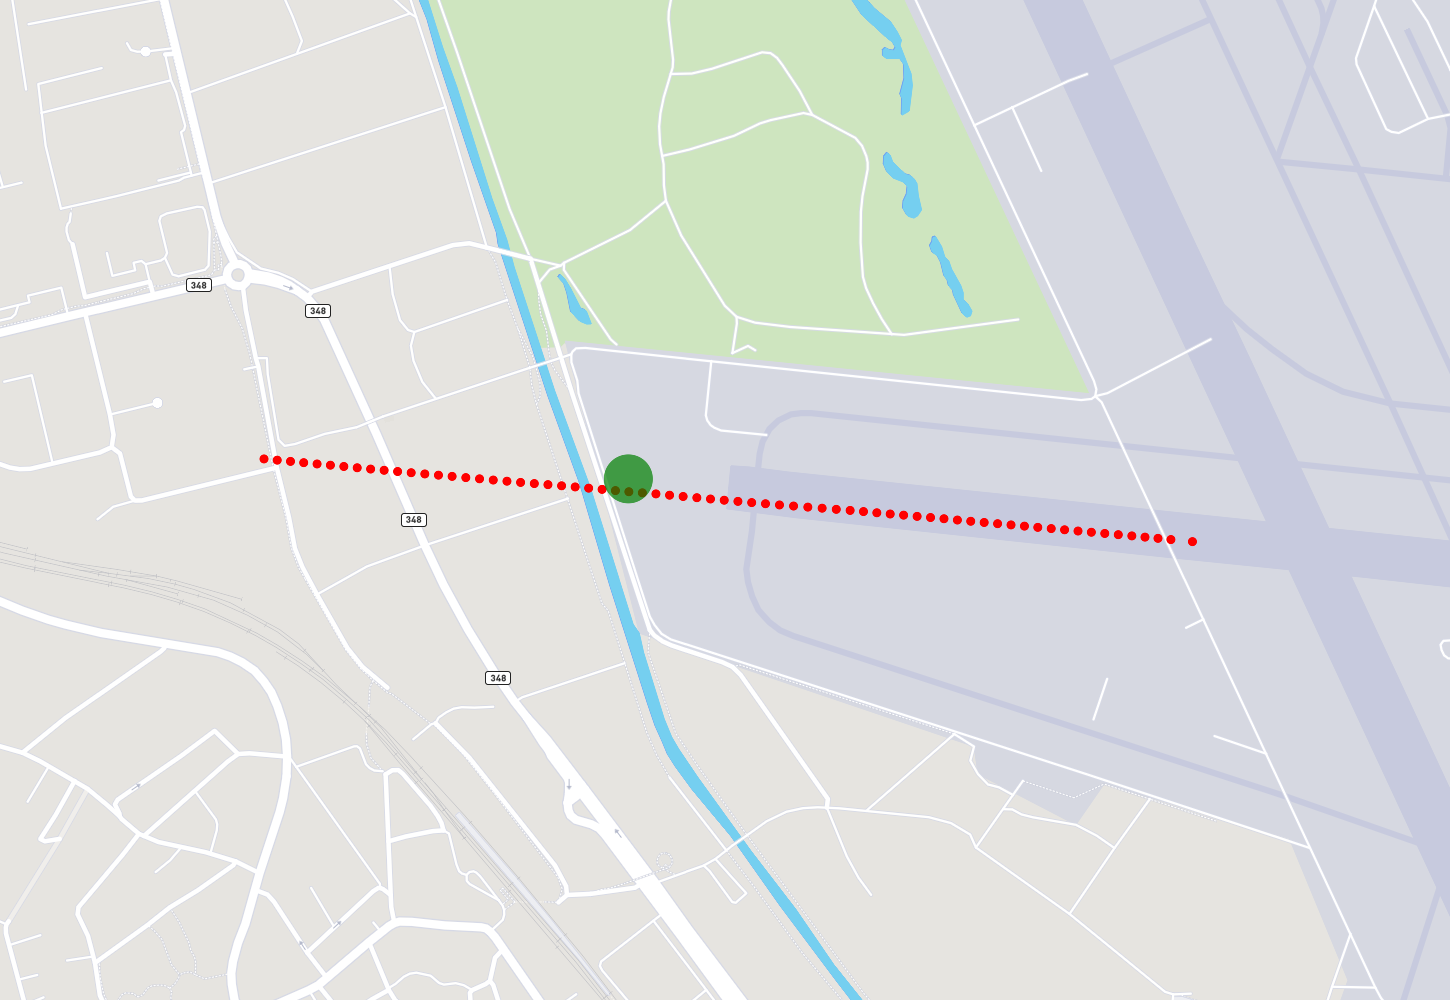
\includegraphics[width=0.3\textwidth]{../figures/manual/auralisation-paper/figure_trajectory}
  \caption{Overview of the airport, trajectory and the receiver. The receiver
(green dot) is situated slightly north of the trajectory, almost straight underneath the
trajectory.}
  \label{fig:figure_trajectory}
\end{figure}


\subsection{Backpropagation}
An automated procedure was developed to backpropagate from receiver to source in
time-domain. The procedure assumes there is only one propagation path,
the direct path, and that the aircraft can be considered a point source.
As shown in Figure \ref{fig:backpropagation_block_diagram}, the
backpropagation algorithm undoes atmospheric attenuation, the Doppler shift, and
geometrical spreading (magnitude) in that specific order, and using the methods as
described in the previous section \cite{Rietdijk2015}.
% A recording is taken, and assuming there were no reflections, the atmospheric attenuation and spherical spreading were undone.
Because only the direct path was considered all parameters that were used in the
backpropagation were based on values corresponding to that path.

\begin{figure}[H]
  \centering
\begin{tikzpicture}[auto, node distance=1cm,>=latex']
\tikzset{
block/.style    = {draw, shape=rectangle, fill=white, minimum height=4em, minimum width=5em, text width=5em, align=center},
}
    % Main nodes
    \node [block]                       (immission)     {Immission\\Recording};
    \node [block, right=of immission]   (attenuation)   {Attenuation\\Filter};
    \node [block, right=of attenuation] (delay)         {Spreading\\Delay};
    \node [block, right=of delay]       (spreading)     {Spreading\\Gain};

    % Main edges
    \draw [->]  (immission)     --  (attenuation);
    \draw [->]  (attenuation)   --  (delay);
    \draw [->]  (delay)         --  (spreading);

\end{tikzpicture}
  \caption{Block diagram of the backpropagation model. These steps are applied sequentially to a recording in order to obtain a signal in time-domain that corresponds to the emission of the aircraft.}
  \label{fig:backpropagation_block_diagram}
\end{figure}

After application of the backpropagation algorithm, a time-domain signal is
obtained that corresponds to the emission of the aircraft. The influence of the
ground reflection is non-negligible. A soft ground is still relatively
hard and therefore a -3 dB correction was applied.

Figures \ref{fig:recording} and \ref{fig:backpropagated} show spectrograms of
respectively the recording and of the signal that was backpropagated. The signal
after backpropagation is shorter than the recording due to lack of aircraft
position information during the initial propagation delay.
Aside from small variations the tonal components remain constant in frequency
over time in Figure \ref{fig:backpropagated}. The variations are caused
by uncertainties in the measured position of the aircraft and thus the estimated
propagation delay.


\begin{figure}[H]
  \centering
  \includegraphics[]{../figures/generated/recording-to-auralisation/recording}
  \caption{
    Spectrogram of a recording of an A320. Clearly visible are the
    Doppler-shifted tones and the peaks due to atmospheric turbulence.
    Interference between direct and reflected path acts as a Comb filter resulting
    in an acoustical Lloyd's mirror-effect, which can be seen here at lower
    frequencies. The most powerful tone corresponds to the blade passing frequency
    of the fan. The other tones are Buzz-Saw tones.}
  \label{fig:recording}
\end{figure}

\begin{figure}[H]
  \centering
  \includegraphics[]{../figures/generated/recording-to-auralisation/reverted}
  \caption{Spectrogram of the recording shown in Figure \ref{fig:recording} after backpropagation to the source. The Doppler-shift has mostly been removed. Artifacts like the mirror-effect and amplitude modulations due to atmospheric turbulence remain.}
  \label{fig:backpropagated}
\end{figure}

\subsection{Feature extraction}
Spectral modelling synthesis was chosen as emission synthesis strategy. With
spectral modelling synthesis a signal is generated as a superposition of tones
and bandpass-filtered noise.
% In order to synthesise the emission of the aircraft
% We're interested in entirely synthesizing the emission of the aircraft and chose to use
% spectral modelling synthesis, that is, a method where a signal is generated
% through a superposition of sines and noise.
Therefore, a method is needed to extract from the backpropagated recordings the
frequency, phase, and level of the tones, as well as the level of the noise as
function of frequency.

A tone-seeking algorithm (in frequency domain) was developed \cite{Rietdijk2016}
that utilises ISO 1996-2:2007 Annex C \cite{ISO1996-2_2007}. The tone-seeking
algorithm as described in the standard did not prove capable of detecting all
tones, and therefore an improved method was needed.

The situations considered are landings, and therefore the tonal components
in the spectra are not only the blade passing frequency of the fan and its
harmonics, but also \say{Buzz-Saw} tones. The common denominator of the frequencies of
these components is the frequency at which the engine shaft rotates.
The assumption was therefore made that all tones found by the
tone-seeking algorithm from the standard were harmonics and that the fundamental
frequency was within a specified range.

The fundamental frequency is given by
\begin{equation}
 f_{0} = \mathrm{gcd}\left(f_1, f_2, \dots, f_n \right)
\end{equation}
where $\mathrm{gcd}$ is the \emph{greatest common divisor}.
Implementations of the $\mathrm{gcd}$ operator attempt to find an exact solution.
Due to errors in the estimation of the frequency of the tones and because some tones are
not harmonics, an exact solution does not exist. Given an initial estimate of
the fundamental frequency, one could define an error as the sum of the squared
deviation between the target order of the harmonics and the actual estimated
order
\begin{equation}
 e = \sum_{i=0}^{n} \left( \frac{f_i}{f_0} - \mathrm{round}\left(\frac{f_i}{f_0}\right) \right)^2
\end{equation}
An estimate of the fundamental frequency is obtained by minimising this error.

An earlier version of the algorithm did not use the $\mathrm{gcd}$ in
combination with the optimisation algorithm but instead determined the
fundamental frequency using the complex cepstrum \cite{Rietdijk2015}.
While it was possible to reliably determine the fundamental frequency with the
complex cepstrum, the value which was obtained was not sufficiently accurate
for determining higher harmonics.

In the method as described in Annex C of ISO 1996-2:2007 each spectral line is
assigned a label, e.g. whether the line is part of a tone or noise. Tones
typically have a bandwidth and can therefore, depending on the frequency
resolution, be spread over multiple lines. In order to compute the level of a
tone, the spectral lines corresponding to that tone need to be integrated.

The bandwidth of the tonal components depends on various aspects, like frequency
or phase modulations at the source or during propagation, e.g. due to
atmospheric turbulence. The direct and reflected contribution are
Doppler-shifted slightly differently and that causes either double peaks or a
single broader peak. But also averaging time and window shape play a role.

The center frequencies of the tonal components obtained with the enhanced method
were fed back in the method of the standard to obtain labels for each spectral
line and to compute the levels of the tones and the noise.
A value for the phase could not be obtained because the signal was too noisy.
The lines that were assigned noise were integrated into \nicefrac{1}{6} octaves and for each
fractional octave its level was kept.

For the feature extraction 2 seconds windows were used, without overlap.
While a short window decreases frequency resolution and precision of the features, a short
window was required in order to provide temporal resolution of the features.
A 2 seconds window proved to be a good balance between temporal resolution
and frequency resolution.

% For the development of an emission model it is expected that
% the uncertainties could be reduced through ensemble averaging. % TODO include this?

\subsection{Emission and immission synthesis}
% As mentioned before the emission was synthesised using spectral modelling
% synthesis.
With the extracted features, which were obtained as function of time and at
several receiver positions, it is possible to develop an emission model that
takes into account directivity of the spectral components. Such emission model
would then output input for the SMS synthesiser and the created emission signal
would be propagated to a receiver a location.

An important question to ask is whether the described methodology of extracting
features, synthesising an emission signal and propagating it would result in
plausible auralisations. For example, it could be possible that the chosen
synthesis strategy and features cannot reproduce certain characteristics in the
sound. Therefore, the next chapter describes a comparison between auralisations
and recordings with the auralisations based on recordings.

For a specific event and receiver, the immission was backpropagated and features
were extracted. These features were used to re-synthesise the emission. The
emission signal was propagated to the receiver, and a direct path and a single
reflection were considered. The assumption was made that the emission is
identical for the emission angles corresponding to direct and reflected path.

The feature extraction method provided frequencies and levels of tonal
components as function of time. Variations in the frequencies as function of
time could be observed, but with a two second window that would result in only
few data points. Variations in frequency were therefore ignored and computed was an
average value for the fundamental and each of the harmonics.

As mentioned in the previous section, values for the phase of the tones could
not be obtained, and therefore values had to be chosen. Because the harmonics
are \say{Buzz-Saw} noise, a phase corresponding to a sawtooth signal was
initially assumed. Participants in a preliminary test found the simulations
sound metallic compared to the recordings \cite{Rietdijk2016a}. Therefore,
eventually a random phase was chosen for each harmonic.

Figures \ref{fig:synthesis} and \ref{fig:auralisation} show spectrograms of
respectively the emission synthesis and the auralisation at the receiver.

\newpage
\afterpage{
\begin{figure}[H]
  \centering
  \includegraphics[]{../figures/generated/recording-to-auralisation/synthesis}
  \caption{Emission synthesis of the aircraft. Inputs to the emission synthesiser were obtained by applying the feature-extraction algorithm to the signal shown in Figure \ref{fig:backpropagated}. The level of the tonal components vary over time. The blade passing frequency is not clearly visible because the determined level of the tone was underestimated.}
  \label{fig:synthesis}
\end{figure}


\begin{figure}[H]
  \centering
  \includegraphics[]{../figures/generated/recording-to-auralisation/auralisation}
  \caption{Auralisation of the event shown in Figure \ref{fig:recording} .
  The Doppler-shifted tones and the mirror-effect are clearly visible. The Doppler-shifted tones are not very smooth. This is due to fluctuations in the aircraft position due to uncertainties.}
  \label{fig:auralisation}
\end{figure}
}


%
%
%
%
%
%
%
%  TODO: BELOW IS OLD STUFF
%
%
% \section{Emission model}
%
% The emission model describes the emission of aircraft. In this section we discuss the development of the model as well as the eventual implementation.
%
% As described in \ref{sec:theory_aircraft_emission_models} several emission models exist.
%
% What is needed for the auralizations is a model that can describe tonal and noise components.
% The models referred to all predict sound levels in fractional-octaves.
%
% Therefore, we will now try to extract the relevant features using an automated method. The method is roughly as follows:
%
% \begin{enumerate}
%  \item Backpropagate from source to receiver in time-domain, undoing the Doppler shift, atmospheric attenuation and spreading. The ground effect is ignored for now. We now have a signal that roughly corresponds to what is emitted from the airplane.
%  \item Determine fundamental frequency. An aircraft spectrum consists mostly of noise and tones, which are mostly harmonics. Knowing the fundamental frequency, allows you to determine the power of not only the fundamental, but also of each harmonic.
%  \item And that is the final step. Determine power of the tones, and consider the rest of the spectrum as noise.
% \end{enumerate}
%
%
%
% \subsection{Empirical model}
% In the sonAir project aircraft landings and take-offs were recorded.
%
% \subsubsection{sonAir data acquisition}
%
% \newpage
% \section{Backpropagation in time-domain}
% To backpropagate in time-domain an inverse propagation model was developed that is based on the propagation model explained in \ref{}.
% The inverse propagation model undoes the intensity loss due to geometrical spreading, as well as the propagation delay that causes the Doppler shift.
% Furthermore, the inverse propagation model corrects for atmospheric attenuation.
% One effect the inverse propagation model cannot undo is the ground effect.
%
%
% \subsubsection{Limitations of the method}
%
%
% \subsubsection{Ground effect}
%
%
%
%
% Now that some of the propagation effects have been undone we have a signal that roughly corresponds to as if you would fly along with the aircraft, and rotate around it.
%
%
% \missingfigure{Spectrum of the recorded signal after backpropagating in time-domain.}
%
% \missingfigure{Power spectrum of the reverted signal.}
%
% \newpage
% \subsection{Determine fundamental frequency}
% To determine the fundamental frequency in an automated and reliable way, several methods were tried.
%
% \subsubsection{Using complex cepstrum}
%
% Using the complex cepstrum it was possible to obtain an accurate estimate for the fundamental frequency \cite{Rietdijk2015}. However, the estimate proved not accurate enough to determine the higher-frequency harmonics.
% Since the frequency of an harmonic is the fundamental multiplied by the order, any inaccuracy in the estimate is multiplied as well. For harmonics around the blade passing frequency and up the error was generally too big.
% Therefore, another method was sought.
%
% \missingfigure{In the complex cepstrum a peak can be found that corresponds to the fundamental frequency.}
%
% \subsubsection{Estimate fundamental from determined tones}
% Estimating the fundamental frequency directly from a spectrum result in an inaccurate estimate. However, when using multiple harmonics, and especially higher order harmonics, the estimate in the error can drop significantly.
%
% \begin{enumerate}
%  \item Determine frequency of harmonics using a tone-seeking algorithm.
%  \item Estimate fundamental frequency given the frequencies of the harmonics.
% \end{enumerate}
%
% An example of a simple tone-seeking algorithm is one that checks when, in the estimate of the power spectrum, the steepness gets above or below a certain threshold. When the threshold is passed twiced - the second sweep in opposite direction - a tone might be present.
% ISO 1996-2:2007 Annex C provides an objective method for assessing the audibility of tones in noise, and part of the method is a tone-seeking algorithm that does exactly this. Aside from the tone-seeking algorithm, the objective method also provides a method for assessing the tones, including estimating their power.
%
% \fbox{\begin{minipage}{0.5\textwidth}
% A method to verify whether audible tones are present in a signal is provided in ISO 1996-2:2007 Annex C. Based on the prominence of tones, the method also provides recommended level adjustments.
% \begin{enumerate}
% \item Find preliminary noise pauses.
% \item Search for tones in noise pauses.
% \item Put a critical band on the centerfrequency of the tone, and determine the tone strength, masking noise level and finally the tonal audibility.
% \item The final tonality adjustment is determined by the tone with the highest tonal audibility.
% \end{enumerate}
% \end{minipage}}
%
% \missingfigure{Tones and critical bands assessed using an implementation of ISO 1996-2:2007 Annex C}
%
% Using a tone-seeking algorithm like the one provided by the standard, one can obtain estimates of the frequencies of tonal components. However, it is not yet known which harmonic order the tone has, or in fact whether it is a harmonic at all.
% Even so, assuming the tones are all harmonic and exact, then the fundamental frequency $f_{0}$ would be the greatest common divisor of the harmonics $f_i$
% \begin{equation}
%  f_{0} = \mathrm{gcd}\left(f_1, f_2, \dots, f_n \right)
% \end{equation}
% Implementations of the $\mathrm{gcd}$ attempt to find an exact solution. However, due to errors in the estimate of the tones (because of a limited frequency resolution) and because some tones are not harmonics, an exact solution would not exist.
% Given an initial estimate of the fundamental frequency, one could define an error as the sum of the squared deviation between the target order of the harmonics and the actual (inaccurate) order
% \begin{equation}
%  e = \sum_{i=0}^{n} \left( \frac{f_i}{f_0} - \mathrm{round}\left(\frac{f_i}{f_0}\right) \right)^2
% \end{equation}
% The fundamental frequency is obtained by minimizing this error. Without constraining the fundamental frequency, incorrect estimates are likely to be obtained. For example, an estimate of the fundamental that is half the actual frequency would fit. And a lower frequency, would also result in a smaller error, causing a preference for a very low-frequency fundamental.
% In our case, we know that the fundamental frequency is generally between 60 and 80 Hz, eliminating both problems.
%
% However, it might still happen that several tones are estimated to be the same harmonic - which is obviously incorrect - and thereby increasing the error in the estimate of the fundamental.
% This can be prevented by checking all combinations with each combination consisting of only unique harmonics. The combination that minimises the error is kept.
%
% The eventual method is:
% \begin{enumerate}
%  \item Estimate frequencies of tones using the tone-seeking algorithm described in ISO 1996-2:2007 Annex C.
%  \item Estimate which harmonic order the tones are.
%  \item Obtain initial estimate of fundamental frequency from the estimated tone frequencies and harmonic orders using a least-squared method. An error is defined as the sum of the absolute deviation between frequency estimate given by 1, and the harmonic order multiplied with the fundamental frequency.
%  \item It might occur that multiple tones would seem to correspond to the same harmonic. This is not possible and should be prevented.
%  \item Therefore all combinations of harmonic order estimates are checked. The result with the smallest error is the final result of the algorithm.
% \end{enumerate}
%
% \newpage
% \subsection{Determine features}
% With the estimate of the fundamental frequency, we also know what the frequencies
% of the harmonics are. The ISO method not only provides an algorithm to determine
% tones, but also a method for assessing them.
%
% We now feed the estimated harmonics back into the ISO method, setting noise
% pause starts and ends at $f_i -/+ f_c/8$. The tone level and bandwidth is is
% determined for each tone, overriding the requirements that frequency lines
% within 6 dB of the maximum should be present, and that the bandwidth should be
% less than 10\% of the critical band.
%
% The frequency of each of these tones is kept as well. The noise lines are
% integrated per fractional-octave.
%
% \begin{table}[h]\centering
%   \caption{Overview of the features.}
%     \begin{tabular}{ | l | l | l | p{5cm} |}
%     \hline
%     Component & Feature & Time-variant \\ \hline
%     Tone & center frequency & yes \\ \hline
%     Tone & bandwidth & yes \\ \hline
%     Tone & sound pressure level & yes \\ \hline
%     Noise & fractional-octave center frequency & no  \\ \hline
%     Noise & fractional-octave band designator & no  \\ \hline
%     \end{tabular}
% \end{table}
%
% \subsubsection{Noise floor}
% The signal-to-noise ratio is dependent on range and thus time. For the samples that were analysed, the noise floor took over at between 8 and 12 kHz.
% For this reason features were only extracted below 8 kHz.
%
% % Knowing the bandpass
% % Furthermore, ISO 1996:2-2007 describes for each frequency line whether it is consider a tone, noise, or neither.
% % This signal can be used to extract relevant features.
% % Many methods exist to detect and track tonal components.
% % ISO 1996-2:2007 Annex C provides an objective method for assessing the audibility of tones in noise.
%
%
% \newpage
% \subsection{Verify features through an auralization}
% Before analysing the features and developing an emission model from them, its important to ask
% the following question. Are these features sufficient to create a realistic
% emission signal? Or, even better, are these features, taking into account the
% developed propagation model, providing a realistic signal at the receiver? Does,
% what you hear, really sound like an aircraft? That is after all the aim.
%
% To verify whether the features contain enough information in order to create a
% plausible auralization, an emission signal was constructed from the features,
% and propagated to the receiver that was used for the measurement.
%
% \subsubsection{Synthesis of emission signal}
% The features that were obtained every second were linearly interpolated to a sample frequency of 22 kHz and were smoothed by applying a rolling mean in both directions.
% The only exception were the frequencies of the harmonics, for which average values were taken. % EXPLAIN!!
% The components are added together resulting in the final signal.
% Figure \ref{} shows a spectrogram of a synthesized emission signal.
%
% \missingfigure{Spectrogram of synthesized emission signal}
%
% \missingfigure{Unweighted sound pressure level as function of time. Fast time-weighting was applied.}
%
% \newpage
% \subsubsection{Signal at receiver}
% We now try to model the propagation of the original event as accurate as
% possible. A virtual receiver is positioned where the real receiver was. Below
% the receiver a flat ground is modelled, disregarding small height differences
% that are present in reality. The ground is modelled to be grass entirely, with
% the impedance calculated using ........
%
% A moving point source follows the original trajectory. The synthesized emission
% signal is now fed directly into the propagation model and is used for both the
% direct path as well as possible reflected paths. The virtual source is modelled
% as a omni-directional source because the synthesis already includes the gain
% adjustment due to source directivity. However, this gain is for a fixed set of
% angles i.e., the angles corresponding to the direct path. For the reflected
% paths the directivity would in reality be slightly different but this effect
% cannot be included in this verification.
%
% Included propagation effects were....
%
% Figure \ref{} shows a spectrogram of a verification auralization as well as a spectrogram of the original recording and figure \ref{} shows the A-weighted sound pressure level as function of time for both.
% \missingfigure{Spectrogram of synthesized emission signal and recording.}
% \missingfigure{A-weighted sound pressure level as function of time. Fast time-weighting was applied.}
%
%
% \newpage
% \subsection{Model}
%





% Subjective validation of synthesis method
\newpage\chapter{Subjective validation of auralisation method}\label{chapter:test}

\section{Introduction}
In the previous chapter an overview was given of the auralisation tool. A
propagation model for aircraft sound was developed but still missing is an
emission model. An algorithm was presented for extracting select features from
recordings with the underlying idea of using those features for the development
of an empirical emission model.

This chapter describes a listening test that was conducted. The purpose of the
listening test was to check the plausiblity or perceptual validity of the
auralisations and a comparison was therefore made between recordings and
auralisations.

The hypothesis is that \emph{recordings and auralisations of aircraft of the same
type and under similar conditions are samples of the same group}.
Audible differences are likely to occur and are also acceptable, because even
among recordings of the same aircraft type there are audible differences.

How sounds are perceived can depend on different factors. Factors can be properties
of the sound, but also of the listener or the environment. Psychoacoustic
measures describe how a sound is perceived by most listeners and can therefore
be used to characterise a sound. Many measures exist, but not all measures are
appliceable to all sounds and care should therefore be taken when choosing
measures. Examples of common measures are loudness, roughness and sharpness.

Due to time-constraints psychoacoustic measures were not measured. Instead, an
overall similarity between stimuli was determined. Recordings were compared not
only with auralisations, but also with other recordings, and similarly,
auralisations with other auralisations. Each of these comparisons can be
considered a group. If the hypothesis is valid, then the distribution of the
group with comparisons between recordings and auralisations, should be the same
as the other two distributions.

% The purpose of the
% test was to determine whether the auralisation tool produces auralisations that
% sound similar to recordings, where the auralisations use for the emission
% synthesis features that were extracted from the recordings. Because the
% available data sets permits simulating and comparing different aircraft types,
% the purpose was also to test whether participants can distinguish between
% aircraft types.
%
% The purpose was not to determine similarity with respect to a certain aspect,
% like for example annoyance, but instead the overall similarity as the goal was to create a tool capable of

% TODO several methods

\section{Method} % This section has been rewritten...slightly.

The goal of the listening test was to determine whether the auralisations sound
similar to the recordings they were based on. Participants were presented with
pairs of stimuli and asked to rate how similar they sounded.

% TODO {explain why this method is chosen? Explain other available methods?}
% One can think of multiple methods to
% determine the similarity. The MUSHRA (MUltiple Stimuli with Hidden Reference and
% Anchor) test is methodology used for evaluating audio quality \cite{}, and has also been used for determining the plausibility of synthesised vehicle pass-by sounds when compared to recordings \cite{Southern2016}.

Eight different sounds were considered and they were each 12 seconds long. The
sounds include the approach of an aircraft, its flyover and its distancing.
Because the character of the sounds varies considerably over time, they were
each split into parts of four seconds, corresponding to the approach, fly-over
and distancing. The listening test was also divided in these three parts. First,
participants were presented to all approach stimuli, then all fly-over stimuli
and finally all distancing stimuli. In each test part all stimuli combinations
were considered. Therefore, each part consisted of 28 pairs of stimuli of four
seconds.

Of the eight sounds four were recordings, and four were auralisations.
The recordings were randomly chosen from the sonAIR dataset. Each
auralisation was based on one of the recordings. Two aircraft types were
considered, an A320 and a RJ1H, as well as two events per aircraft type.
Fade in and fade out was applied to the stimuli. The signals were mono and
presented with headphones. Head-related transfer functions were not included.

Similarity is relative, and therefore an anchor is typically used. For each
part, participants were first given the set of stimuli, in order to become
familiar with the type of sounds and the spread in the sounds of that part, and
then continued with rating the pairs. The rating was done on an eleven point
Likert scale. The left side of the scale said ``not so much'' and the right side
``very much''. The scale was not numbered. The order of the stimuli was
randomised for each test and each part.

Figures \ref{fig:listening:results:recording-A320} and
\ref{fig:listening:results:simulation-A320} show spectrograms of some of the stimuli
that were used. The blade passing frequency and harmonics are not as prominent
in the auralisation as they are in the recording.

% \newpage
% \afterpage{
\begin{figure}[H]
  \centering
  \includegraphics[]{../figures/generated/listening/recording-A320}
  \caption{Spectrograms of the approach, fly-over and distancing parts of a recording of an A320.}
  \label{fig:listening:results:recording-A320}
% \end{figure}
%
% \begin{figure}
  \centering
  \includegraphics[]{../figures/generated/listening/turbulence-A320}
  \caption{Spectrograms of the approach, ``center`` and distancing parts of an auralisation of an A320.}
  \label{fig:listening:results:simulation-A320}
\end{figure}
% }
% \clearpage

\newpage
\section{Results}
The results of the participants were scaled linearly from 0 to 1 with 0
corresponding to ``not so much'' and 1 corresponding to ``very much''.
% Not all of the participants used the entire scale, and therefore they were rescaled per
% participant and per test part to use the full scale.
There were 17 participants, all graduate students, and of which the majority
studied acoustics. The results that are shown are obtained after joining the
data of all participants. % and all three test parts.
% Update raw results??
The listening test data can be found at \cite{Rietdijk2017a} and the
raw results along with a brief analysis at \cite{Rietdijk2017b}.

Table \ref{table:listening:results:analysis-parts} shows the mean $\mu$,
standard deviation $\sigma$ and amount of samples $n$ per group.
Averaging was done over participants. Table \ref{table:listening:results:analysis} is similar,
but now averaging was done not over only participants but also over the three test parts.

\begin{table}[H]
  \centering
  \caption{The mean value $\mu$, standard deviation $\sigma$ and amount of samples $n$ per aircraft type combination, and stimuli type combination. Averaging was done over participants and parts.}
  \label{table:listening:results:analysis}
  \input{../figures/generated/listening-analysis/table_analysis.tex}
\end{table}

Figure \ref{fig:listening:ratings-kde-overall} shows the distribution of the
similarity ratings grouped by aircraft and stimuli type combinations. The
vertical axes show kernel density estimations of how common the given ratings
were\footnote{ A kernel density estimation can be seen as a continuous version
of a histogram. Each sample is replaced by a kernel function centered at the
value of the sample. The curves are then summed to obtain a density and finally
normalised so that the area under the resulting curve is 1. }. A Gaussian kernel
was used. Averaging is done over participants and test parts.

Figures \ref{fig:listening:ratings-aircraft-type-combinations} and \ref{fig:listening:ratings-stimuli-type-combinations} show mostly the same curves as Figure \ref{fig:listening:ratings-kde-overall} but the curves are grouped.
Figure \ref{fig:listening:ratings-aircraft-type-combinations} shows the distribution of the similarity ratings grouped by
aircraft combination for both the recordings and the auralisations.
Figure \ref{fig:listening:ratings-stimuli-type-combinations} shows the distribution of the similarity ratings grouped by stimuli type combination
for both the A320 and the RJ1H. In both cases the results encompass all parts.

\begin{figure}[H]
  \centering
  \includegraphics{{{../figures/generated/listening-analysis/figure_kde}}}
  \caption{Similarity ratings grouped by both aircraft combinations and stimuli type combinations.}% Groups considering only recordings and compare only one aircraft type have relatively high similarity ratings. Groups that consider two aircraft types have relatively the lowest ratings. }
  \label{fig:listening:ratings-kde-overall}
\end{figure}

In Figures \ref{fig:listening:results:ratings-A320-parts} and
\ref{fig:listening:results:ratings-RJ1H-parts} the results were split by part.
To improve clarity, the amount of information is reduced by using Tukey boxplots.

Participants mentioned they noted larger differences at especially the approach of the events and the distancing.
A common answer to the question how many different aircraft they heard was ``two or three``.
Occasionally, the answer would start at ``two`` but go to ``two or more`` after they
were told they were listening to not only recordings but also simulations. Some
participants were surprised when told that simulations were included,
others said they had thought so, and a few of the participants were already
aware the test was possibly going to contain simulations.

\begin{table}[H]
  \centering
  \caption{The mean value $\mu$, standard deviation $\sigma$ and amount of samples $n$ per test part, aircraft type combination, and stimuli type combination. Averaging was done over participants.}
  \label{table:listening:results:analysis-parts}
  \input{../figures/generated/listening-analysis/table_analysis_parts.tex}
\end{table}


% \newpage
% \afterpage{
\begin{figure}
%     \centering
    \begin{subfigure}{0.5\textwidth}
        \includegraphics{{{../figures/generated/listening-analysis/figure1_ratings_recordings}}}
        \caption{Recordings}
        \label{fig:listening:ratings-aircraft-type-combinations:recordings}
    \end{subfigure}
    \begin{subfigure}{0.5\textwidth}
        \includegraphics{{{../figures/generated/listening-analysis/figure2_ratings_simulations}}}
        \caption{Auralisations}
        \label{fig:listening:ratings-aircraft-type-combinations:auralisations}
    \end{subfigure}
    \caption{Similarity ratings grouped by aircraft type combinations. The left figure shows the ratings for the recordings and the right figure for the auralisations.}
    \label{fig:listening:ratings-aircraft-type-combinations}
% \end{figure}
% \clearpage

% \begin{figure}
    \begin{subfigure}{0.5\textwidth}
        \includegraphics[]{{{../figures/generated/listening-analysis/figure3_ratings_A320}}}
        \caption{A320}
        \label{fig:listening:ratings-stimuli-type-combinations:A320}
    \end{subfigure}
    \begin{subfigure}{0.5\textwidth}
        \includegraphics[]{{{../figures/generated/listening-analysis/figure4_ratings_RJ1H}}}
        \caption{RJ1H}
        \label{fig:listening:ratings-stimuli-type-combinations:RJ1H}
    \end{subfigure}
    \caption{Similarity ratings grouped by stimuli type combinations. The left figure shows the ratings for the A320 and the right figure for the RJ1H.}
    \label{fig:listening:ratings-stimuli-type-combinations}
\end{figure}
% }
% \clearpage

% \begin{figure}[H]
%   \centering
%   \includegraphics[]{../figures/generated/listening-analysis/figure1_ratings_recordings}
%   \caption{Similarity ratings for the recordings grouped by aircraft type.}
%   \label{fig:ratings_recordings}
% \end{figure}
%
% \begin{figure}[H]
%   \centering
%   \includegraphics[]{../figures/generated/listening-analysis/figure2_ratings_simulations}
%   \caption{Similarity ratings for the auralisations grouped by aircraft type.}
%   \label{fig:ratings_simulations}
% \end{figure}
%
% \begin{figure}[H]
%   \centering
%   \includegraphics[]{../figures/generated/listening-analysis/figure3_ratings_A320}
%   \caption{Similarity ratings for the A320 grouped by stimuli type combinations.}
%   \label{fig:ratings_A320}
% \end{figure}
%
% \begin{figure}[H]
%   \centering
%   \includegraphics[]{../figures/generated/listening-analysis/figure4_ratings_RJ1H}
%   \caption{Similarity ratings for the RJ1H grouped by stimuli type combinations.}
%   \label{fig:ratings_RJ1H}
% \end{figure}


%
% \newpage
% \afterpage{
% \begin{float}
\begin{figure}[H]
  \centering
  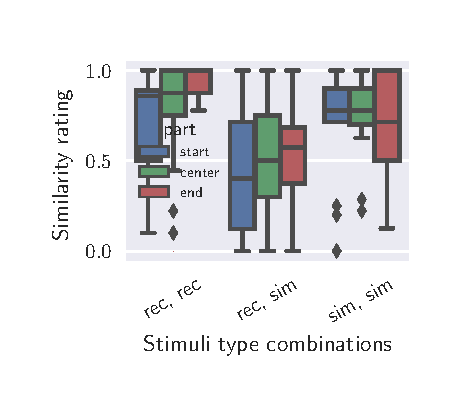
\includegraphics[]{../figures/generated/listening-analysis/figure5_ratings_part_A320}
  \caption{Similarity ratings for the A320 grouped by stimuli type combinations and stimuli part.}
  \label{fig:listening:results:ratings-A320-parts}
% \end{figure}
% TODO discuss

% \begin{figure}[H]
  \centering
  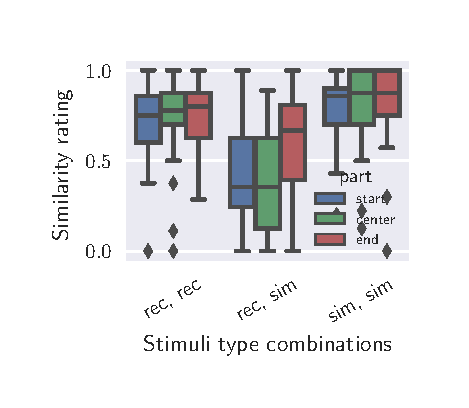
\includegraphics[]{../figures/generated/listening-analysis/figure6_ratings_part_RJ1H}
  \caption{Similarity ratings for the RJ1H grouped by stimuli type combinations and stimuli part.}
  \label{fig:listening:results:ratings-RJ1H-parts}
\end{figure}
% \end{float}
% TODO discuss
% }

\newpage
\section{Discussion}
Consider Tables \ref{table:listening:results:analysis} and
\ref{table:listening:results:analysis-parts}. The standard deviation of the
groups is mostly around 0.25, although a notable exception is the group in which
two recordings of A320's were compared. The standard deviation is only 0.09 and
the mean 0.89. Comparing that with the other groups, implies the two recordings
this group consists of are relatively closer to eachother than those in other
groups.
The highest mean values are achieved when comparing similar aircraft types,
regardless of whether the stimuli were recordings or auralisations. However,
when comparing a recording with an auralisation the mean value is lower. The
mean values of the groups comparing recordings and auralisations are
systematically below those of the groups comparing recordings or auralisations.
That would imply the hypothesis is not true.

Figure \ref{fig:listening:ratings-kde-overall} shows kernel density estimates of
the distributions of the nine groups. Some groups appear to follow a Gaussian
curve, however, not all. In certain cases there are also (close to) two maxima.
The similarity rating is a value given by participants after performing a
comparison of two items, and comparing them on whichever aspects they choose to
consider. Therefore, it is likely that the distributions are Gaussian. However,
because the ratings could only be given on a limited range this may skew the
distributions.

% Z-score and p-value?

As can be seen in Figure
\ref{fig:listening:ratings-aircraft-type-combinations:recordings}, the recordings of the A320's
are judged to be very similar to each other, and the recordings of the RJ1H's as quite similar to
each other as well. The A320's are not rated as very similar to the RJ1H's and therefore
it appears that the participants can discriminate between the two aircraft
types.
In the case of the auralisations, Figure
\ref{fig:listening:ratings-aircraft-type-combinations:auralisations}, the
results are similar in case of the A320's and the RJ1H's, although less convincing.
Furthermore, in this case the dissimilarity between the A320's and the RJ1H's isn't as large.
In fact, this distribution is relatively closer to the other two distributions than is the case with the recordings,
implying the auralisations, regardless of aircraft type, all sound more alike.

% participants can also discriminate between the aircraft types, but now the
% RJ1H's are judged to be relatively more similar than the A320's. Compared to the
% recordings the difference between the A320's and the RJ1H's is slightly smaller.

% One might argue from these findings that the whole set of auralisations is more similar than the set of recordings.

Another view on the data is presented in Figure
\ref{fig:listening:ratings-stimuli-type-combinations}. Were the hypothesis
valid, then the curves in each subfigure would have to overlap. While the
distributions of the groups that compare auralisations are quite similar to the
distributions comparing recordings, the groups comparing auralisations with
recordings are not similar at all. That would again imply the hypothesis is not
true and that the auralisations may appear to be different types of aircraft.

% The groups ``(rec, sim)'' contain pairs consisting of a recording and an auralisation, and the similarity ratings of these two groups are similar to the ``(A320, RJ1H)''
% groups in Figure \ref{fig:listening:ratings-aircraft-type-combinations}. Therefore,
% it would appear that listeners can discriminate between aircraft types, but that
% the auralisations are considered to be of different aircraft types than the
% recordings they are based on.

Figures \ref{fig:listening:results:ratings-A320-parts} and
\ref{fig:listening:results:ratings-RJ1H-parts} show the same data as \ref{fig:listening:ratings-stimuli-type-combinations}
but grouped further by stimuli part. Judging from Figure
\ref{fig:listening:results:ratings-A320-parts} there appears to be a
relative large dissimilarity between the approach and fly-over parts of the A320 recordings.
The distancing parts, however, are rated as very similar. The groups ``(rec,
rec)'' and ``(sim, sim)'' consist however of only 17 data points.

% When comparing auralisations
% and recordings there does not seem to be any especially good or bad part: the spread is relatively large and the mean is mediocre at
% and also between the ``end'' parts of the A320 auralisations.  each whereas
% the ``(rec, sim)'' group has 68 data points.

The participants mentioned relatively larger differences in the stimuli that
correspond to the approach of the aircraft (``start`` stimuli). During the
approach the tonal components are clearly audible compared to other parts of the
events due to the directivity. The feature-extraction algorithm was known to
underestimate the power and bandwidth of the blade passing frequency and its
harmonics because the algorithm was tuned for the Buzz-Saw tones. Therefore, a
likely explanation is that this underestimation of power and bandwidth is
causing audible differences between recordings and auralisations.
Furthermore, as described in section \ref{sec:tool:synthesis:synthesis}, an
incorrect distribution was used for the phase relation between the harmonics.

Finally, it should be noted that only two events per aircraft type were
considered. In a future test more events should be considered in order to
correctly represent the spread that exists in recordings of a certain aircraft
type.


% Modelling propagation in a turbulent atmosphere
\newpage\chapter{Propagation in a turbulent atmosphere}\label{chapter:turbulence} % TODO From paper. Rewrite

\section{Introduction}
Spatial and temporal variations in the atmosphere affect sound propagation and
can cause audible modulations. Because they can be clearly audible it is
presumed that including scintillations in auralisations increases their
perceived realism. The multiple scattering affects the phase of the signal as
well as the log-amplitude. In previous work a coherence factor was introduced
that would account for coherence loss due to phase modulations \cite{Shin2006,
Arntzen2014b, Arntzen2014a}. Fluctuations due to turbulence have also been
included in auralisations by simulating the amplitude modulations that were
observed in measurements \cite{Heutschi2014, Minard2016}.

This chapter describes a method, published in Paper \ref{paper:turbulence}, for
generating sequences of scintillations and including them in auralisations. The
method considers line-of-sight propagation through a weakly turbulent
atmosphere. Novel in this field, the method includes both log-amplitude and
phase fluctuations. The presented method is based on \cite{Jurado-navas2006}
where it was used to predict the performance of wireless communication links,
and \cite{Forssen2000} where it was used to determine the influence of
turbulence on the performance of a barrier. An early version of the method was
discussed in Papers \ref{paper:forum2014} and \ref{paper:asa2014}.
Furthermore, the method was implemented in the NAF\cite{Aumann2017}.

% \newpage
% \section{Wave propagation in random media}

\section{Coherence loss factor}
Before presenting the new method let us consider an existing method that was
mentioned in the introduction. Arntzen developed a method to include coherence
loss \cite{Arntzen2014a,Arntzen2014b}, and the method considers a coherence factor $T_c$, first described by
Clifford and Lataitis \cite{Clifford1983}, as well as a reciprocal filter $R_c$.
Consider a typicaly scenario of a direct path and ground-reflected path. The
sound pressure at the receiver is given by
\begin{equation}
%   p = \frac{A_d}{r_d} e^{j(\left(k r_d \right) + \phi_d} + Q \frac{A_r}{r_r} e^{j(\left(k r_r \right) + \phi_r}
  p = \frac{A_d}{r_d} e^{j k r_d } + Q \frac{A_r}{r_r} e^{j k r_r }
\end{equation}
where $A$ is an amplitude, $r$ a path length, $Q=|Q|\exp{(j\phi)}$ a reflection
factor (in the referred work the spherical reflection factor), and the indices $d$ and $r$ are used to represent respectively the
direct and reflected paths. Note the amplitude can be different for each path to account for source directivity.
% If $A_d=A_r=A$, then the pressure relative to free field $p/p_0$ is
% \begin{equation}
%   \frac{p}{p_0} = 1 + Q \frac{r_d}{r_r} e^{-jk\left( r_r - r_d \right)}
% \end{equation}
The effective pressure squared, as used for computing a sound pressure level, is
\begin{equation}
%   p_{e}^2 = \frac{1}{r_d^2} +  \frac{|Q|}{r_r^2} +  \frac{2 |Q|}{r_d r_r} \cos{\left(k \left( r_r - r_d \right) + \phi + \phi_r - \phi_d \right)}
  p_{e}^2 = \frac{A_d^2}{2 r_d^2} + |Q|^2 \frac{A_r^2}{2 r_r^2} + 2 |Q| \frac{A_d A_r}{r_d r_r} \cos{\left(k \left( r_r - r_d \right) + \phi  \right)}
\end{equation}
The sum of the first and second term is an incoherent addition of the direct and
ground-reflected contributions. The third term on the right-hand side considers
the interference between the direct and reflected paths.

Clifford and Lataitis considered atmospheric turbulence in a line-of-sight
propagation situation and accounted for complex phase perturbations, i.e.
log-amplitude and phase, for each propagation path. They introduced a coherence
factor $T_c$ in the third term to include additional coherence loss due to
atmospheric turbulence in line-of-sight propagation
\begin{equation}
  p_{e}^2 = \frac{A_d^2}{2 r_d^2} + |Q|^2 \frac{A_r^2}{2 r_r^2} + 2 |Q| T_c \frac{A_d A_r}{r_d r_r} \cos{\left(k \left( r_r - r_d \right) + \phi  \right)}
\end{equation}
The factor ranges from zero to one and can nullify interference.
Assuming a spherical wave front and a Gaussian turbulence spectrum, the coherence factor is given by
\begin{equation}
  T_c = e^{-\sigma_S^2 \left(1 - C_{sp}\right)}
\end{equation}
where $\sigma_S^2$ is the variance of phase fluctuations (equation
\eqref{eq:model_daigle}), and $C_{sp}$ the phase correlation (equation
\eqref{eq:theory:propagation:turbulence:correlation}. The phase correlation is a function of the spatial separation $\rho$
perpendicular to the wave propagation direction which in this case was derived as
\begin{equation}
  \frac{1}{\rho} = \frac{1}{2} \left( \frac{1}{h_s} + \frac{1}{h_r}  \right)
\end{equation}
where $h_d$ and $h_r$ are respectively the source and receiver height.
The variance $\sigma_S^2$ is the sum of the direct and reflected path phase variances \cite{Clifford1983}.

The interference term is implicitly included in auralisations. Therefore,
Arntzen included $T_c$ as a filter for the ground-reflected path and introduced
another reciprocal filter $R_c$.
\begin{equation}
  p = R_c \frac{A_d}{r_d} e^{j\left(k r_d \right) } + Q T_c \frac{A_r}{r_r} e^{j\left(k r_r \right) }
\end{equation}
The magnitude-response of the reciprocal filter is given by
\begin{equation}
  R_c = - |Q| T_c + \sqrt{|Q|^2 + 2 |Q| T_c + 1}
\end{equation}
and is needed because the ground-reflected wave would be lost in case $T_c$ approached
zero, which will happen with strong turbulence, i.e., high values of
$\sigma^2_S$.

A qualititive validation showed that the model indeed results in audible and
predictable coherence loss, reducing the rasping sound due to interference that
was otherwise clearly audible, and thereby increasing the perceptual validity.

\section{Generating sequences of scintillations}

Atmospheric turbulence is known to result in not only coherence loss but also in
audible amplitude modulations. We shall therefore now explore a new method that
also includes audible amplitude modulations. Whereas the method from the
previous section modified the magnitude of the coherent part to increase
coherence loss, the method proposed in this section generates sequences of
log-amplitude and phase fluctuations and applies these to each propagation path.

\subsection{Space-to-time conversion}

Consider again a line-of-sight situation where
$d$ is the distance between a source and a receiver pair along the wave
propagation direction, and $\rho$ the spatial separation of the receivers
transverse to the wave propagation direction.
Still assuming Taylor's hypothesis regarding frozen turbulence, we can perform a
space-to-time conversion of the correlation and covariance functions to obtain
$C(\tau)$ and $B(\tau)$ respectively. The turbulence correlation time is given
by
\begin{equation}
 \tau_0 = \frac{L}{v_{\bot}}
\end{equation}
and the transverse time lag by
\begin{equation}
  \tau = \frac{\rho}{v_{\bot}}
\end{equation}
where $v_{\bot}$ is the transverse speed, corresponding to e.g. the mean speed
at which the field is carried by the wind transverse to the wave propagation
direction.

In this chapter the covariance for spherical waves and a Gaussian spectrum is
considered for the same reason it was used in the other method: the Gaussian
spectrum is the simplest model to work with and computationally least demanding.
The method can also be used with covariance functions that describe other
turbulence spectra, like e.g. the Von Karman spectrum \cite{Ostashev2015}.

\subsection{Propagation in the turbulent atmosphere as a multichannel}
The fluctuations in the atmosphere are temporal and/or spatial. Therefore, to
model sound propagation of a signal $x(t)$ through such an atmosphere a
time-varying channel is necessary. The received signal $y(t)$ consists of a
line-of-sight contribution and additional contributions from scattering,
together forming a multichannel \cite{Jurado-navas2006}.
Ignoring beam spreading, this can be written as %The received signal can be written as the sum of $n$ channels
\begin{equation}
 y(t) = \sum_{n} \alpha_{sc_{n}}(t) x(t-\tau_n(t))
\end{equation}
where $\alpha_{sc_{n}}(t)$ is the time-varying scintillation sequence
representing the effect of the pressure fluctuations on the $n$th-multipath
component, and $\tau_n$ the propagation delay of the $n$th component relative to the propagation delay in an undisturbed atmosphere.
Assuming the spread in propagation delay over the channels is small compared to the inverse of the signal bandwidth, so that $x(t-\tau_n) \approx x(t - \tau(t))$, then
\begin{equation}
 y(t) = x(t - \tau(t)) \sum_n \alpha_{sc_{n}}(t)
\end{equation}
Because the attenuation is very similar for the different multipaths, we can write that
\begin{equation}\label{eq:generating_sequences_multiplicative}
 y(t) = x(t - \tau(t)) \alpha_{sc}(t)
\end{equation}
Therefore, the received signal is obtained by shifting the emitted signal $x(t)$ with a time-varying propagation delay $\tau(t)$, and multiplying the result with a time-varying gain $\alpha_{sc}(t)$.


\subsection{Design of scintillation sequence}
We will now design a sequence of scintillations and for that we need to know the
statistical distribution and power spectral density $|H_B(f)|^2$ of the desired
sequence. As mentioned before the fluctuations are Gaussian-distributed. We can
therefore generate a sequence with the correct distribution and power spectral
density by convolving a random unit variance Gaussian signal $z(t)$ with the
impulse response $h_B(t)$ of the designed filter.
\begin{equation}
 \chi(t) = S(t) = (h_B \ast z)(t)
\end{equation}

The power spectral density $|H_B(f)|^2$ of a random sequence forms a Fourier pair
with its autocorrelation function $R(\tau)$ through the Wiener-Khinchin
theorem\footnote{The Wiener-Khinchin theorem states that the autocorrelation
function of a wide-sense-stationary random process has a spectral decomposition
given by the power spectrum of that process.}. Assuming $R(\tau) \cong B_{\chi}(\tau)=B_{S}(\tau)$,
the power spectral density of $\chi$ and $S$ is
\begin{equation}
 |H_B(f)|^2 = \int_{-\infty}^{\infty} B(\tau) \exp{\left(-j\omega \tau\right)} \mathrm{d}\tau
\end{equation}
This filter has zero phase and is non-causal. To create a causal filter
with constant group delay $\alpha$ we can shift the peak in the impulse response
by adding a linear-phase factor corresponding to 90 degrees
\begin{equation}
 H_B(f) = |H_B(f)|  \cdot \exp{\left(-j 2\pi f \alpha\right)}
\end{equation}
The impulse response of the filter is finally obtained through the Inverse Fourier Transform
\begin{equation}
 h_B(t) = \int_{-\infty}^{\infty} H_B(f) \exp{\left(+j\omega \tau\right)} \mathrm{d}\tau
\end{equation}

\subsection{Discrete time}
We now convert from continuous to discrete time
\begin{equation}
 H_B[k] = H_B(e^{j\omega}), \quad 0 \leq k \leq N-1, \quad  \omega = \frac{2 \pi k}{N}
\end{equation}
The linear-phase factor $\exp{\left(-j 2\pi f \alpha\right)}$ is then given by
\begin{equation}
 \exp \left\{ -j 2\pi k \frac{M_1}{2} \frac{f_s}{N} \right\}
\end{equation}
where $M_1$ is the length of the desired impulse response. The frequency response of the filter is
\begin{equation}\label{eq:discrete_time_filter}
 H_B[k] =  \sqrt{ F \left\{  B[n] \right\}  } \exp \left\{ -j 2\pi k \frac{M_1}{2} \frac{f_s}{N} \right\},  \quad 0 \leq k \leq N/2
\end{equation}
where $F\{\}$ is the Discrete Fourier Transform (DFT).
The desired impulse response is real-valued. Therefore, we have because of Hermitian symmetry
\begin{equation}
\begin{aligned}
 &H_B[k] = H_B(e^{j\omega}), &\quad 0 &\leq k \leq N/2, \quad  \omega = \frac{2 \pi k}{N} \\
 &H_B[N-k] = H_B^{*} [k], &\quad 1 &\leq k \leq N/2 - 1
\end{aligned}
\end{equation}
In fact, because both $B[n]$ and $|H_B[k]|$ are real and even, one can use the type-1 Discrete Cosine Transform (DCT) instead of the DFT in equation \eqref{eq:discrete_time_filter}.
The impulse response of the filter is obtained by taking the Inverse Discrete Fourier Transform (IDFT)
\begin{equation}
 \begin{aligned}
 h_B[n] &= F^{-1} \left\{ H_B[k] \right\} \\
  &= F^{-1} \left\{ \sqrt{ F \left\{  B[n] \right\}  } \exp \left\{ -j 2\pi \frac{M_1}{2} k \frac{f_s}{N} \right\} \right\}
\end{aligned}
\end{equation}
Scintillations are finally obtained through the convolution of the impulse response $h_B[n]$ with Gaussian white noise $z[n]$
\begin{equation}\label{eq:scintillations_convolution_discrete}
 \chi[n] = S[n] = (z \ast h_B ) [n]
\end{equation}
The first $M_1/2$ samples would have to be dropped because of the filter delay.
A block diagram of the steps is shown in Figure \ref{fig:generating_block_diagram_simple}.

\begin{figure}[H]
  \centering
\begin{tikzpicture}[auto, node distance=2cm,>=latex']
\tikzset{
op/.style       = {draw, shape=circle, fill=orange, minimum height=2em, minimum width=2em},
block/.style    = {draw, shape=rectangle, fill=white, minimum height=3em, minimum width=3em},
coord/.style    = {coordinate},
}

    % Fluctuations nodes
    \node [op]                (fluct_conv)    {$\ast$};
    \node [coord, left=of fluct_conv]      (fluct_noise)   {};

    % Fluctuations edges
    \draw [->] (fluct_noise)-- node{$z[n]$}                 (fluct_conv);

    % Filter nodes
    \node [block, right=of fluct_conv]      (fluct_idft)    {IDFT};
    \node [block, right=of fluct_idft]      (fluct_spectrum){$\sqrt{\quad}$};
    \node [block, right=of fluct_spectrum]  (fluct_dft)     {DFT};
    \node [coord, right=of fluct_dft]       (fluct_ac)      {};
    % Filter edges
    \draw [->] (fluct_idft) --node{$h_B[n]$} (fluct_conv);
    \draw [->] (fluct_spectrum) -- node{$|H_B[k]|$} (fluct_idft);
    \draw [->] (fluct_dft) -- node{$|H_B[k]|^2$} (fluct_spectrum);
    \draw [->] (fluct_ac) -- node{$B[n]$} (fluct_dft);

    \node [coord, below=of fluct_conv]      (fluctuations)   {};
    \draw [->] (fluct_conv)-- node{$\chi[n]=S[n]$}                 (fluctuations);

\end{tikzpicture}
  \caption{Block diagram of signal processing steps for generating scintillations. Gaussian white noise $z[n]$ is convolved with an impulse response $h_B[n]$ which is based on the covariance $B[n]$ of the turbulence spectrum.}
  \label{fig:generating_block_diagram_simple}
\end{figure}

\subsection{Apply scintillations to signal}
Now that we can generate sequences of fluctuations, we need to apply these to a
carrier signal $x(t)$ or $x[n]$. According to equation
\eqref{eq:generating_sequences_multiplicative} the log-amplitude fluctuations can
be applied in a multiplicative manner, which is indeed the case of a signal with
a sufficiently small bandwidth, like for example a monochromatic signal.
However, the variance of the fluctuations is frequency-dependent, and since in
practice broadband signals are commonly used, a method is sought for applying the
fluctuations to a broadband signal.

One possible method would be to decompose the input signal in complex
exponentials with the Inverse Discrete Fourier Transform, and apply per complex
exponential the log-amplitude and phase fluctuations which, when combined, can be
written as a complex exponential $\psi$ as shown in equations
\eqref{eq:complex_exponential} and \eqref{eq:chi_and_S}.

A computationally less demanding method is to instead filter the carrier signal
with multiple band-pass filters, and proceed with applying fluctuations to each
of the band-pass filtered signals and combining the resulting signals.
Scintillations would be computed for the center frequencies of the bands. The amplitude
fluctuations could be applied through multiplication and the phase
fluctuations could be converted to time-delay fluctuations (see equation
\eqref{eq:time_delay_fluctuations}) and applied with a Variable Delay Line.


\subsection{Scintillations as time-variant filter}
A more efficient method to take into account the frequency-dependence
of the scintillations, would be to instead convolve the carrier signal with a
time-variant filter that is updated fast enough to represent the fluctuations.

The fluctuations $\chi$ and $S$, at each time step computed for $M_2$ frequencies, can be merged into a complex phase (see equation \eqref{eq:chi_and_S})
\begin{equation}
 \psi[n] = \exp\left({\chi[n] + jS[n] }\right)
\end{equation}
Adding a linear-phase factor as was done with $h_B[n]$ and taking the Inverse
Discrete Fourier Transform will result in an impulse response for every instance
in time $n$. Convolution of the carrier signal $x[n]$ with this time-variant
filter will result in a log-amplitude and phase modulated signal. The first
$M_2/2$ samples will have to be dropped to correct for the filter delay.

Because the fluctuations are relatively low-frequent they can be sampled at a
much lower sample frequency than the carrier signal. For a correlation length
$L$ of 10 meters and a transverse speed $v_{\bot}$ of 2 meters per second the
correlation time would be 5 seconds. If we would sample the sequence of
fluctuations at 5 times the maximum bandwidth of the filter, which is
proportional to the inverse of the correlation time $\tau_0$,
\begin{equation}
 f_s = 5 / \tau_0
\end{equation}
the required sample frequency would be 1 hertz.

In practice one might want to interpolate the impulse response as it changes
over time, but because the phase also changes with time this can be problematic.
Aside from converting to a minimum-phase representation\footnote{
A system is minimum-phase when it and its inverse are both causal and stable, which would require both the poles and zeros to be inside the unit circle.
The group delay is minimal and thus its energy is concentrated at the start of an impulse response.} we can also create a
linear-phase filter for which the magnitude changes with time but the phase does
not. If the phase fluctuations are linear-phase, then they can be applied to the
carrier signal $x[n]$ with a Variable Delay Line. In the Gaussian model the
phase fluctuations scale as $\sigma_S^2 \sim f^2$. A scatterer affects all frequencies, and therefore the fluctuations of different frequencies move together, resulting in a linear-phase.
We therefore write the phase fluctuation $\mathrm{d}S(t)$ as a propagation delay fluctuation
\begin{equation}\label{eq:time_delay_fluctuations}
\mathrm{d}t(t) = \mathrm{d}S(t) / (2 \pi f)
\end{equation}
% TODO How does this fit with the channel, eqs. 19-22
or in discrete time
\begin{equation}
 \mathrm{d}[n] = \mathrm{d}S[n] / (2 \pi k f_s)
\end{equation}

With the Gaussian turbulence spectrum it is straightforward to separate the
covariance $B(\tau)$ into the correlation $C(\tau)$ and variance $\sigma$ as defined in respectively equations \eqref{eq:gaussian_correlation} and \eqref{eq:model_daigle}. That
way we can compute a filter $h_C[n]$ that depends solely on the correlation
$C(\tau)$, and scale this afterwards with the correct variances $\sigma_{\chi}$
and $\sigma_{S}$. The advantage is having to compute only one sequence of
fluctuations, which is determined entirely by the covariance and $z[n]$, and can
then be scaled with the (frequency-dependent) variances $\sigma_{\chi}$ and
$S$.

\subsection{Moving source}
Thus far it was assumed neither the source nor the receiver were moving, and
that the fluctuations arise due to sampling a turbulent field that is moving
by with constant speed at a fixed receiver position.

If the field is transported faster, the spatial fluctuations are sampled faster,
and therefore the scintillations $\chi[n]=S[n]$ are compressed in time
corresponding to fluctuations with relatively higher frequencies.

In case the turbulent field is transported by wind and neither source nor
receiver are moving, the source-receiver distance remains constant. If we
instead consider a moving source of which the emitted sound samples the turbulent field, then the
source-receiver distance $d$ generally changes and thus also the variances $\sigma_{\chi}$ and $\sigma_{S}$.

We will now consider a moving source. The transverse velocity is in this case
the velocity component of the moving source, perpendicular to the wave
propagation direction. This is the vector \emph{rejection} of the source
velocity vector $\mathbf{v_s}$ from the unit vector $\mathbf{\hat{o}}$ that
represents the orientation from source to receiver. The transverse speed is the
norm of this vector
\begin{equation}
 v_{\bot} = \left\| \mathbf{v_s} - (\mathbf{v_s} \cdot  \mathbf{\hat{o}} ) \cdot \mathbf{\hat{o}}  \right\|
%  v_{\bot} = \left\| \mathbf{\hat{o}} \times \mathbf{v_s} \right\|
\end{equation}
The vector \emph{projection} of the source velocity on the wave propagation
direction is the component that is relevant for the Doppler shift. Therefore, as
the Doppler shift is maximum the modulations are relatively low-frequent,
whereas if the Doppler shift is zero, the modulations are relatively
high-frequent.

When computing two sequences of scintillations, but for different
transverse speeds, one does not obtain a compressed version of the other using
the method as described thus far in this section, even when using the same seed
for the Pseudo-Random Number Generator. This is because, by adjusting $v_{\bot}$,
we effectively applied the compression on the filter $h_C[n]$ before convolution
with $z[n]$. Therefore, the two resulting sequences will not look compressed in
time, but instead just filtered differently. Even so, the generated sequence will
have the desired statistical properties.

We can obtain the desired compression, i.e., scaling in time, if we instead
perform the convolution between $z[n]$ and a time-invariant $h_C[n]$ computed for a fixed $\tau_0$, $\tau_{\mathrm{ref}}$, and then
resample the values of $\chi[n]$ and $S[n]$ at different times to take into
account the change in correlation. Instead of having a constant sample timestep
\begin{equation}
 t_k = \frac{k}{f_s} = \sum_{i=0}^k \frac{1}{f_s}, \quad k=0, 1, \dots, \quad i=0, 1, \dots
\end{equation}
the sample time varies with correlation time
\begin{equation}
  t_k = \sum_{i=0}^k \frac{\tau_{\mathrm{ref}}}{\tau_{0,i}} \frac{1}{f_s} , \quad k=0, 1, \dots, \quad i=0, 1, \dots
\end{equation}

Figure \ref{fig:generating_block_diagram} shows the full block diagram of the signal
processing steps for generating scintillations and including them in an auralization.


\subsection{Saturation of the log-amplitude fluctuations}
According to equation \eqref{eq:model_daigle} the fluctuations increase with distance and frequency indefinitely.
For longer path lengths or stronger turbulence, the amplitude fluctuations
gradually level off. Saturation of the amplitude fluctuations can be observed
when measuring aircraft noise at distances of over a few kilometers. The
standard deviation of the fluctuating sound pressure levels is in such cases
limited to approximately 6 dB \cite{Daigle1983}.

Saturation of the log-amplitude fluctuations can be included based on an analysis by Wenzel
\cite{Wenzel1975}. In Wenzel's approach the soundwave is split up in a coherent
and incoherent wave. The amplitude of the coherent wave decreases over distance
while the incoherent wave obtains the energy from the coherent wave. The
coherent wave $p$ is written as
\begin{equation}
 \langle p \  p^* \rangle = \left( A_m^2 / 4 \pi r^2 \right) \exp{\left( -2 \langle \mu^2 \rangle k^2 r L \right)}
\end{equation}
Wenzel defines the distance to saturation $r_s$ as the distance at which the coherent wave is reduced to $e^{-1}$ of its original strength
\begin{equation}\label{eq:saturation_distance}
 r_s = \frac{1}{2 \sigma_{\mu}^2 k^2 L}
\end{equation}
Saturation of the log-amplitude fluctuations can now be included by multiplying the log-amplitude with a correction factor.
The variance of log-amplitude fluctuations that includes saturation $\sigma_{\chi}$, is given by
\begin{equation}\label{eq:saturation_logamp}
 \sigma_{\chi, sat} = \sigma_{\chi} \frac{ 1}{1 + r/r_s}
\end{equation}

\begin{figure}[H]
  \centering
\begin{tikzpicture}[auto, node distance=2cm,>=latex']
\tikzset{
op/.style       = {draw, shape=circle, fill=orange, minimum height=2em, minimum width=2em},
block/.style    = {draw, shape=rectangle, fill=white, minimum height=3em, minimum width=3em},
coord/.style    = {coordinate},
}
    % Apply nodes
    \node [op]              (apply_conv) at (-2, 0)   {$\ast$};
    \node [coord, left=of apply_conv]                           (input)         {};
    \node [block]      (apply_vdl) at (+2, 0)    {VDL};
    \node [coord, right=of apply_vdl]       (output)        {};

    % Apply edges
    \draw [->] (input)      -- node{$x[n]$}                 (apply_conv);
    \draw [->] (apply_conv) --                              (apply_vdl);
    \draw [->] (apply_vdl)  -- node{$y[n]$}                 (output);

    % Amplitude nodes
    \node [block, above=of apply_conv]      (apply_ir)      {IDFT};
    \node [block, above=of apply_ir]        (a_exp)         {exp};
    \node [op, above=of a_exp]              (a_apply_var)   {$\times$};
    \node [coord, left=of a_apply_var]      (a_var)         {};
    \node [coord]     (a_tee) at (-2, 10)      {};

    % Amplitude edges
    \draw [->] (a_tee)      -- node{$\chi_{\sigma=1}[n]$}            (a_apply_var);
    \draw [->] (a_var)      -- node{$\sigma_{\chi}[k]$}  (a_apply_var);
    \draw [->] (a_apply_var)-- node{$\chi[k]$}            (a_exp);
    \draw [->] (a_exp)      -- node{$e^{\chi[k]}$}        (apply_ir);
    \draw [->] (apply_ir)   -- node{$h[n]$}               (apply_conv);

    % Phase nodes
    \node [op, above=of apply_vdl]          (p_to_delay)    {$\times$};
    \node [op, above=of p_to_delay]         (p_apply_var)   {$\times$};
    \node [coord, right=of p_apply_var]     (p_var)         {};
    \node [coord, right=of p_to_delay]      (p_delay)       {};
    \node [coord]     (p_tee)  at (+2, 10)       {};

    % Phase edges
    \draw [->] (p_to_delay) -- node{$\mathrm{d}t[n]$}       (apply_vdl);
    \draw [->] (p_apply_var)-- node{$S[k]$}              (p_to_delay);
    \draw [->] (p_var)      -- node{$\sigma_S[k]$}        (p_apply_var);
    \draw [->] (p_delay)    -- node{$\frac{1}{2 \pi k}$}    (p_to_delay);
    \draw [->] (p_tee)      -- node{$S_{\sigma=1}[n]$}               (p_apply_var);

    % Fluctuations nodes
    \node [coord] (tee) at (0, 10) {};
    \node [block, above=of tee]                (fluct_resample)     {Resample};
%     \node [coord, right=of a_tee]           (tee)           {};
    \node [op, above=of fluct_resample]                (fluct_conv)    {$\ast$};
    \node [coord, left=of fluct_conv]      (fluct_noise)   {};
    \node [coord, left=of fluct_resample] (correlation_time_rel) {};

    \draw [->] (correlation_time_rel) -- node{$\frac{\tau_{\mathrm{ref}}}{\tau_{0}}[n]$}  (fluct_resample);

    % Fluctuations edges
    \draw [->] (fluct_noise)-- node{$z[n]$}                 (fluct_conv);
    \draw [->] (fluct_conv) --                              (fluct_resample);
    \draw [->] (fluct_resample)  --                              (tee);
    \draw [-]  (tee)        --                              (a_tee);
    \draw [-]  (tee)        --                               (p_tee);

    % Filter nodes
    \node [block, right=of fluct_conv]      (fluct_idft)    {IDFT};
    \node [block, right=of fluct_idft]      (fluct_spectrum){$\sqrt{\quad}$};
    \node [block, below=of fluct_spectrum]  (fluct_dft)     {DFT};
    \node [coord, below=of fluct_dft]       (fluct_ac)      {};
    % Filter edges
    \draw [->] (fluct_idft) --node{$h_{C}[n]$} (fluct_conv);
    \draw [->] (fluct_spectrum) -- node{$|H_C[k]|$} (fluct_idft);
    \draw [->] (fluct_dft) -- node{$|H_C[k]|^2$} (fluct_spectrum);
    \draw [->] (fluct_ac) -- node{$C[n]$} (fluct_dft);


\end{tikzpicture}
  \caption{Block diagram of signal processing steps.}
  \label{fig:generating_block_diagram}
\end{figure}

\section{Results}

\subsection{A single tone}
To demonstrate the model we shall now consider a tone of 1000 Hz and apply modulations to the tone.
The following parameters are used: $c=343.2$
m/s, $\sigma_{\mu}^2=3\cdot10^{-6}$, $L=1.1$ m, $v_{\bot}=2.0$ m/s and $d=500$
m. Saturation according to equation \eqref{eq:saturation_logamp} is also included.
The filter $h_c$ is designed to have 8192 taps. The correlation time is then
$\tau=L/v_{\bot}=0.55$ s and the sample frequency at which the modulations are
generated $5/\tau=9.1$ Hz.

Figure \ref{fig:results_tone_logamp_and_phase} shows the time series of
amplitude and phase fluctuations that were generated. Figure
\ref{fig:results_tone_levels} shows the tone along with a modulated version of
the tone. The tone was sampled at 8000 Hz.

The log-amplitude and phase move in-phase. The value for the log-amplitude is slightly lower than that of the phase because of saturation.
As expected the phase fluctuations cause spectral broadening of the tone as can be seen in Figure \cite{Ostashev2016}.

\begin{figure}[H]
  \centering
  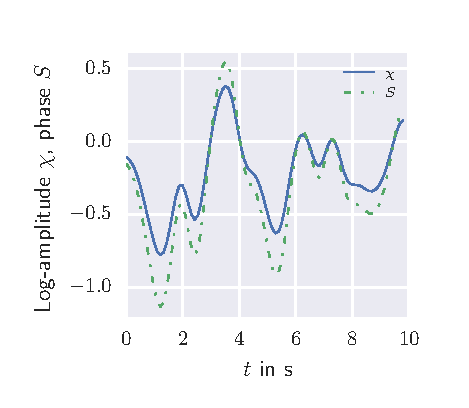
\includegraphics[]{../figures/generated/turbulence-tone/logamp_and_phase}
  \caption{Amplitude and phase fluctuations as function of time. The fluctuations are less strong for the amplitude fluctuations due to saturation.}
  \label{fig:results_tone_logamp_and_phase}
\end{figure}

\begin{figure}[H]
  \centering
  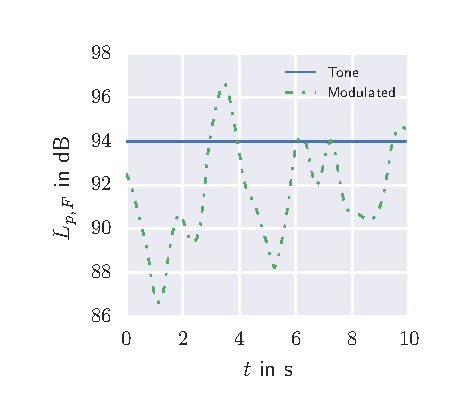
\includegraphics[]{../figures/generated/turbulence-tone/modulated_levels}
  \caption{Sound pressure level of the tone as function of time, with and without fluctuations.}
  \label{fig:results_tone_levels}
\end{figure}



\begin{figure}[H]
  \centering
  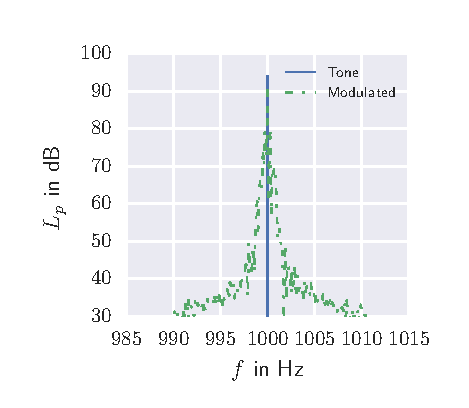
\includegraphics[]{../figures/generated/turbulence-tone/tone_broadening}
  \caption{The power spectrum of the tone shows the broadening due to the phase fluctuations although the bandwidth at -3 dB from the maximum is still small.}
  \label{fig:results_tone_broadening}
\end{figure}

\subsection{Scintillations as function of transverse speed}
By changing the transverse speed the refractive-index field is sampled at a
different speed. This effectively changes the correlation length and shifts the frequency range that is covered by our applied filter \cite{Wilson1999}.

Figure \ref{fig:results_scintillations_correlation} shows the correlation function for
different transverse speeds.
\begin{figure}[H]
  \centering
  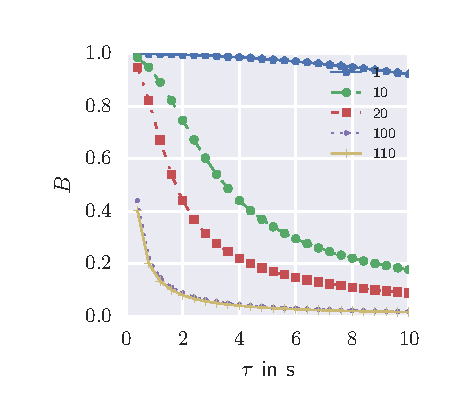
\includegraphics[]{../figures/generated/turbulence-tone/correlation}
  \caption{Correlation as function of time for different transverse speeds given in meters per second.}
  \label{fig:results_scintillations_correlation}
\end{figure}
With a high transverse speed the correlation drops
faster, and this will result in relatively more high-frequency fluctuations, as is shown in Figure \ref{fig:results_scintillations_levels}.
\begin{figure}[H]
  \centering
  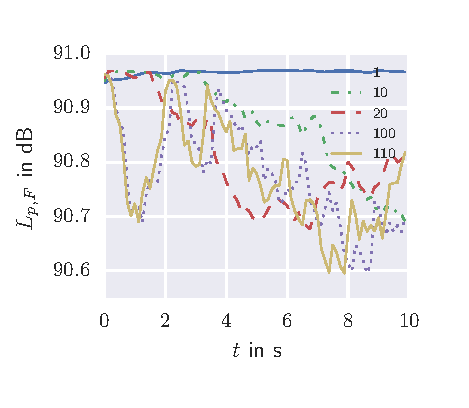
\includegraphics[]{../figures/generated/turbulence-tone/scintillations_levels}
  \caption{Sound pressure level as function of time for scintillations
corresponding to different transverse speeds given in meters per second. The
same $z[n]$ were used for each case. A compression in time of the modulations with increasing velocity can be observed.}
  \label{fig:results_scintillations_levels}
\end{figure}


\subsection{Application in auralisation of aircraft}
The method was developed in order to create more plausible sounding
auralizations of aircraft. An aircraft moves at high speed through the
atmosphere. A transverse speed is computed for each propagation path separately.
Because the correlation time, distance and propagation varies between the two
paths, decorrelation occurs. Figures \ref{fig:results_auralization_without} and
\ref{fig:results_auralization_with} show spectrograms, respectively with and
without turbulence. The vertical lines that can be seen are the amplitude
modulations.

\begin{figure}[H]
  \centering
  \includegraphics[]{../figures/manual/turbulence-model/auralisation_flight_without}
  \caption{Spectrogram of an auralisation of an aircraft taking off.
Scintillations were not included. Visible are the ground effect and the Doppler
shift. In the initial seconds a high amount of tonal components are visible.
  }
  \label{fig:results_auralization_without}
\end{figure}

\begin{figure}[H]
  \centering
  \includegraphics[]{../figures/manual/turbulence-model/auralisation_flight_both}
  \caption{Spectrogram of the same event as in Figure
  \ref{fig:results_auralization_without}, however, this time with scintillations included. Because of the high speed at which the aircraft samples the refractive-index field the scintillations are relatively high-frequent, resulting in vertical lines.}
  \label{fig:results_auralization_with}
\end{figure}

Earlier it was assumed that the correlation length was much smaller than the
Fresnel zone size. In this auralisation the aircraft is moving close to the
receiver. When the aircraft is closest, the distance is almost entirely given by
the height which was approximately 100 meters. The correlation length was set at
20 meters. In that case the Fresnel zone is larger than the correlation length
for the lower frequencies, and equation \eqref{eq:model_daigle} is not valid.
Instead, the log-amplitude and phase variances should scale with respectively
$d^3$ and $2k^2 d$ instead of $k^2 d$.

\subsection{Influence of parameters}
The two main parameters of the Gaussian model are the variance of
refractive-index fluctuations $\sigma^2_{\mu}$ and the correlation length $L$.
Figures \ref{fig:turbulence:aircraft:parameters:correlation} and
\ref{fig:turbulence:aircraft:parameters:variance} show examples of the effect of each of
these parameters on an auralisation of an "aircraft".

\begin{figure}[H]
%     \centering
    \begin{subfigure}{\textwidth}
        \includegraphics{{{../figures/generated/turbulence-parameters/turbulence-1.0-1e-05}}}
        \caption{\SI{1}{\meter}}
    \end{subfigure}
    ~
    \begin{subfigure}{\textwidth}
        \includegraphics{{{../figures/generated/turbulence-parameters/turbulence-4.0-1e-05}}}
        \caption{\SI{4}{\meter}}
    \end{subfigure}
    ~
    \begin{subfigure}{\textwidth}
        \includegraphics[]{{{../figures/generated/turbulence-parameters/turbulence-16.0-1e-05}}}
        \caption{\SI{16}{\meter}}
    \end{subfigure}
    \caption{The influence of the correlation length $L$. The variance of the dynamic refractive-index is fixed at $\SI{1e-5}{}$. A higher correlation length results in slower fluctuations.}
    \label{fig:turbulence:aircraft:parameters:correlation}
\end{figure}

\newpage
\begin{figure}[H]
%     \centering
    \begin{subfigure}{\textwidth}
        \includegraphics{{{../figures/generated/turbulence-parameters/turbulence-1.0-1e-05}}}
        \caption{\SI{1e-5}{}}
    \end{subfigure}
    ~
    \begin{subfigure}{\textwidth}
        \includegraphics{{{../figures/generated/turbulence-parameters/turbulence-1.0-1e-06}}}
        \caption{\SI{1e-6}{}}
    \end{subfigure}
    ~
    \begin{subfigure}{\textwidth}
        \includegraphics[]{{{../figures/generated/turbulence-parameters/turbulence-1.0-1e-07}}}
        \caption{\SI{1e-7}{}}
    \end{subfigure}
    \caption{The influence of the variance of the dynamic refractive-index $\sigma_{\mu}^2$. The correlation length is fixed at \SI{1}{\meter}. A higher variance results in stronger fluctuations.}
    \label{fig:turbulence:aircraft:parameters:variance}
\end{figure}


\section{Conclusion}
Fluctuations in the refractive-index field due to variations in temperature and
wind affects sound propagation and causes audible modulations. A method was
presented for generating sequences of modulations and applying these to
monochromatic as well as broadband signals.

A Rytov approximation to first-order refractive-index flucutuations results in a complex
phase which we can write as a log-amplitude $\chi$ and phase $S$ fluctuation.
The propagating sound is modelled as a time-varying channel where we consider
two sequences, one for the log-amplitude fluctuations, and another for the phase
fluctuations.

The fluctuations are frequency-dependent and therefore a filter was designed to take that into account.
% A Gaussian applied filter was used to model the atmospheric turbulence because of its simplicity and because it is computationally least demanding.
A Gaussian turbulence spectrum was considered, but the general method can be
used with other turbulence spectra as well. The Von Karman spectrum describes
real turbulence spectra typically better than the Gaussian spectrum, however,
the Von Karman spectrum is computationally much more demanding.
% The Gaussian model also allows implementing the phase fluctuation with a Variable Delay Line (VDL).

Examples are shown where the method is applied to a tone and to an aircraft
auralization. The aircraft auralisation spectrogram shows several spikes
corresponding to amplitude modulations as well as an increase in the amount of
decorrelation. Furthermore the transverse velocity dependence on the frequency
content of the modulations is demonstrated.

According to the author the method results in more plausible sounding
auralizations, but this has not been validated yet with listening tests.




% Conclusions
\chapter{Conclusions and future work}\label{chapter:conclusions}

\section{Conclusions}

% TODO: comment Jens, sounds plausible

\todo{remove sections}
\subsubsection{Auralization paper}\todo{rewrite and merge}
In order to investigate the impact of aircraft sound on humans a tool was
developed to auralise aircraft sound. The goal was to develop a tool that can
create auralisations that sound similar to the target aircraft and is capable of
creating auralisations of the current fleet of aircraft.

A propagation model based on geometrical acoustics was developed and the
emission synthesis was based on features extracted from recordings with the use
of an inverse propagation model and a feature extraction algorithm. A listening
test was conducted to determine whether the chosen features are sufficient for
creating auralisations that sound similar to the actual aircraft.

From the listening test it follows that listeners can discriminate between
sounds of different aircraft types, in case of both recordings and
auralisations. The similarity ratings between recordings and auralisations are
similar to the similarity ratings between the two aircraft type, implying the
auralisations sound like different aircraft than those that were recorded.
The dissimilarity between the auralisations and recordings is believed to be
caused by the incorrect reproduction of the blade passing frequency and its
harmonics caused by an underestimation of the power and bandwidth during the
feature-extraction.

Section \ref{sec:introduction:background:auralisation} listed several
auralisation use cases. Whether it is relevant that the auralisations do not
sound exactly similar to the recordings would depend on how the auralisations
would be utilised.

\subsubsection{Turbulence paper}\todo{rewrite and merge}
To improve the plausibility of the auralisations
% in situations where the source-receiver distance is typically larger
a method was developed to simulate for auralisations modulations
due to atmospheric turbulence. Fluctuations in the refractive-index field due to
variations in temperature and wind affects sound propagation and causes audible
modulations. A method was presented for generating sequences of modulations and
applying these to monochromatic as well as broadband signals.

A Rytov approximation to first-order refractive-index fluctuations results in a complex
phase which we can write as a log-amplitude $\chi$ and phase $S$ fluctuation.
The propagating sound is modelled as a time-varying channel where we consider
two sequences, one for the log-amplitude fluctuations, and another for the phase
fluctuations.

The fluctuations are frequency-dependent and therefore a filter was designed to take that into account.
% A Gaussian applied filter was used to model the atmospheric turbulence because of its simplicity and because it is computationally least demanding.
A Gaussian turbulence spectrum was considered, but the general method can be
used with other turbulence spectra as well. The Von Karman spectrum describes
real turbulence spectra typically better than the Gaussian spectrum, however,
the Von Karman spectrum is computationally much more demanding.
% The Gaussian model also allows implementing the phase fluctuation with a Variable Delay Line (VDL).

Examples are shown where the method is applied to a tone and to an aircraft
auralization. The aircraft auralization spectrogram shows several spikes
corresponding to amplitude modulations as well as an increase in the amount of
decorrelation. Furthermore the transverse velocity dependence on the frequency
content of the modulations is demonstrated.

The method seems to result in more realistic sounding
auralizations, but this has not been validated yet with listening tests. The
implementation of the model that was used in this paper to generate the figures
can be found at \cite{Rietdijk2016}.

\section{Future work}
Future steps to be taken depends strongly on how auralisations would
be used.
% The next steps to be taken depend on how auralisations would be used.

\subsubsection*{Investigate human response to aircraft sound}
If one wants to study humans' response to aircraft sound, then the next step is
to test whether auralisations of aircraft are sufficiently similar to the actual
sound of aircraft, with respect to the parameter that is being investigated. If
the conclusion is that auralisations and recordings give sufficiently similar
results, then that would imply the auralisation method can be used to further
study that aspect of human response within the domain that was considered. If
significant differences would still be found, it would have to be tested what is
causing the differences.

% TODO comment Jens
% Future work: I suggest to add some example for the reader, at "If one wants to study humans’ response to aircraft sound, then the next step is to test whether auralisations of aircraft are sufficiently similar to the actual sound of aircraft, with respect to the parameter that is being investigated", like e.g. ", e.g. perceived annoyance or sleep disturbance."

\subsubsection*{Improve estimation and synthesis of blade passing frequency}
From the study that was conducted and presented in this work, it followed that
participants did indeed notice differences between the auralisations and the
recordings. A probable cause of these differences is the estimation of the
power and bandwidth of the blade passing frequency and harmonics. Therefore, a
possible improvement would be to enhance the feature-extraction algorithm to
better estimate these properties.

% The most important point to improve is likely the simulation of the
% blade passing frequency and harmonics, and that would require a better
% estimation of their powers and bandwidths. Aside from that, it would seem the
% auralisation tool is capable of delivering plausible auralisations.

\subsubsection*{Develop generic aircraft emission model}
Because the auralisations appear to sound plausible it is concluded that the strategy\todo{what strategy? recording, backprop, ...}
utilised works and therefore


\subsection{Scintillations}

\subsubsection*{Validate scintillations model}
The scintillations model is based on an existing statistical model.

\subsubsection*{Different model for describing turbulence spectrum}
As mentioned in the text the basic method for generating scintillations should
also work with other models, like the Von Karman spectrum. The Gaussian model
was chosen for performance reasons, as its simplest, but also because it allowed
further optimisations. Future work could be to develop an optimised algorithm
that utilises other spectra like e.g. the Von Karman spectrum with the use of
expressions given in \cite{Ostashev2015}.

\subsubsection*{Non-isotropic and non-homogeneous atmosphere for the scintillations model}
% \subsubsection*{Height-dependent parameters for the scintillations model}
The current model assumes a isotropic and homogeneous atmosphere. In practice,
the atmosphere is neither and parameters like the correlation length $L$ and the
variance of the refractive-index fluctuations $\langle \mu^2 \rangle$ are
height-dependent \cite{Krasnenko2013}. Ostashev et al. gave formulas for plane
\cite{Ostashev1997b} and spherical \cite{Ostashev1997c} waves propagating
through an anisotropic atmosphere and studies numerically the variances and
correlation functions of the log-amplitude and phase fluctuations
\cite{Ostashev2004}.

\subsubsection*{Determine parameters for scintillations model}
The model that was presented for generating scintillations uses a Gaussian
correlation function. A Gaussian can be used as an applied filter to get a rough
approximation to the actual turbulence spectrum within a certain wavenumber
range. An open question is how to obtain adequate values for the correlation
length $L$ and the variance of the refractive-index fluctuations $\langle \mu^2
\rangle$. Values for both can be obtained with a setup as used by Daigle et. al.
\cite{Daigle1983}, however, with such a setup values can only be obtained at
relatively low heights.




% \subsection{Develop better indicators for annoyance and sleep disturbance}

% \chapter{Future work}



    \printbibliography[heading=bibintoc]

  \end{refsection}

\cleardoublepage

% % % Preparations before Part II. In this part one chapter = one paper

\renewcommand{\chaptername}{Paper}
                              % write 'Paper' instead of 'Chapter' in the title

\setcounter{chapter}{0}       % reset chapter numbers after Part I

% Fix hyperlinks to chapters/papers after chapter counter reset, see
% http://tex.stackexchange.com/a/6099
\renewcommand\theHchapter{appendedPaper.\arabic{chapter}}

\renewcommand{\thesection}{\arabic{section}}
                              % exclude chapter number from section number
                              % Figures, Tables, etc are still prefixed by chapter number.
                              % For algorithms numbering see definition of
                              % \newfloat{algorithm} above.

% \newcommand{\paper}[7]
% % #1 Paper Title
% % #2 Short Title for page headers (ToC has the full title)
% % #3 Label for later (or earlier) \ref:s
% % #4 Authors
% % #5 Where published
% % #6 Comment (like "reprinted with a kind permission" and "reformatted for uniformity")
% % #7 File to input
% {
%   \chapter{#1\label{#3}}      % Title as Chapter
%   \chaptermark{#2}            % Short title for the page header
%   \thispagestyle{empty}       % no page numbers
%   {\Large #4}\par             % authors
%   \vspace{1cm}
%   \noindent\emph{\Large #5}\par % where published
%   \vspace{3cm}
%   \noindent\emph{\Large #6}   % Comment
%   \cleardoublepage            % skip back side of the page
%   \thispagestyle{plain}       % no header above paper title
%   \begin{center}
%     {\Large \bfseries Paper~\thechapter. #1}\par % title again
%     \vspace{1pc}
%     #4 \par                   % authors again
%     \vspace{3pc}
%   \end{center}
%   \begin{refsection}          % start of biblatex's refsection for sub-bibliography
%   \input{#7}                  % paper itself, starting from abstract (no title)
%   \printbibliography[heading=subbibintoc] % biblatex bibliography
%   \end{refsection}            % end of biblatex refsection
% }

% \newcommand{\reformatted}{The paper was reformatted for uniformity, but otherwise is unchanged.}
%
% % \part{Appended papers}        % in this part one chapter = one paper
%
% % Example of using the command \paper defined above:
% \paper{SAT-solving in practice, with a tutorial example from supervisory control}
%       {SAT-solving in practice, with a SCT example}
%       {pap:supervisory}
%       {Koen~Claessen, Niklas~Een, Mary~Sheeran, Niklas~Sörensson, Alexey~Voronov and Knut~Åkesson}
%       {Journal of Discrete Event Dynamic Systems (2009), 19(4): 495--524.}
%       {Reproduced with kind permission from Springer Science+Business Media. \reformatted}
%       {paper-supervisory/body}
%
% \paper{The same paper, inserted second time for illustration}
%       {SAT-solving in practice, with a SCT example}
%       {pap:another-one}
%       {Koen~Claessen, Niklas~Een, Mary~Sheeran, Niklas~Sörensson, Alexey~Voronov and Knut~Åkesson}
%       {Journal of Discrete Event Dynamic Systems (2009), 19(4): 495--524.}
%       {Reproduced with kind permission from Springer Science+Business Media. \reformatted}
%       {paper-supervisory/body}

\chapter*{Paper \ref{paper:turbulence}}
\fullcite{Rietdijk2017}
\includepdf[pages=-]{../papers/2017_turbulence}
\chapter*{Paper \ref{paper:overview}}
\fullcite{Rietdijk2017c}
\includepdf[pages=-]{../papers/2017_overview}
\chapter*{Paper \ref{paper:internoise2016}}
\fullcite{Rietdijk2016a}
\includepdf[pages=-]{../papers/2016_internoise}
\chapter*{Paper \ref{paper:euronoise2015}}
\fullcite{Rietdijk2015}
\includepdf[pages=-]{../papers/2015_euronoise}
\chapter*{Paper \ref{paper:forum2014}}
\fullcite{Rietdijk2014}
\includepdf[pages=-]{../papers/2014_forum}
\end{document}
